% Formato para un capítulo cualquiera

%Título del capítulo
\chapter{Introducción} 
\label{sec:intro}
 
Según expresa Soderblom en \cite{Soderblom10}, se pueden medir muchas de las propiedades físicas claves de las estrellas. La masa se puede determinar a partir de la física básica o también se puede inferir a partir de un tipo espectral, particularmente para la secuencia principal. La composición de las estrellas, que no es fácil de determinar pero, se puede seguir un proceso bien comprendido y se conocen sus limitaciones. Sin embargo, la edad, que es el tercer determinante clave del estado físico de una estrella, no se puede medir directamente, solo se puede estimar. Únicamente se tiene la edad precisa y exacta de una estrella, el Sol. Pero esta edad no ha sido revelada por la propia estrella sino que, se consigue limitar gracias a la posibilidad de estudiar en un laboratorio la materia que compone el sistema solar. Estudio que no se puede hacer para ninguna otra estrella.

En algunas ocasiones, es posible determinar las edades si se colocan ciertos eventos en la secuencia correcta y se es capaz de comprender la duración relativa de cada una de las fases. Pero, normalmente se necesitan unir observaciones de objetos o sucesos independientes para alcanzar la comprensión de un proceso. Como por ejemplo:

\begin{itemize}
\item La formación y evolución de los discos protoplanetarios parece ocurrir en los primeros 100 Myr de la vida de una estrella, y los discos de escombros se forman más tarde. En la actualidad, apenas se puede limitar esta escala temporal con los métodos disponibles, y para comprender la física de los procesos implicados, es necesario observar las diferencias en los procesos de formación y conocer la escala temporal entre ellos, además del de las estrellas implicadas.
\item Se han descubierto muchos planetas gigantes gaseosos alrededor de estrellas de tipo solar cercanas. Para obtener una mejor comprensión de, por ejemplo, la dinámica de tales sistemas y la migración hacia el interior de los planetas, se requieren edades precisas.
\item Se podría comprender mejor el comportamiento y el futuro de nuestro Sol si pudiéramos crear una verdadera cohorte basada en la masa, la composición y la edad. En la actualidad, las comparaciones del Sol con otras estrellas a menudo se basan en las propiedades estelares, el proceso es autorreferencial.
\item Para comprender completamente la historia de formación, enriquecimiento y dinámica de la Galaxia, se necesita poder asignar edades a las estrellas individuales. Las estrellas de baja masa viven lo suficiente para estar presentes en todas las épocas de formación estelar, lo que las hace atractivas para estos fines.
\item La búsqueda de vida y cualquier comprensión obtenida al observar signos de vida más allá de nuestro sistema solar tiene una profunda necesidad de medir las edades estelares si se espera obtener información sobre la evolución biológica.
\end{itemize}

La comprensión completa de una gran variedad de fenómenos astrofísicos significa que, al menos, se conoce la secuencia correcta de eventos y sus correspondientes escalas de tiempos. Muchos de estos fenómenos están relacionados con estrellas individuales o conjuntos de estrellas cercanas, por lo que se necesitan formas confiables de llegar a las edades de estos objetos.

Partiendo de que la edad es la propiedad más difícil de obtener, ya que es la única que no se puede observar \emph{directamente} en nigún caso y debe inferirse utilizando diversos métodos. Soderblom presentó dos estudios que describen la mayoría de estas técnicas \cite{Soderblom15, Soderblom10}.

Dentro del grupo de aproximaciones para la datación estelar, una de las técnicas más prometedoras es la girocronología o datación de estrellas mediante su periodo de rotación. Las estrellas nacen con un rango de velocidades de rotación por diferentes razones físicas, ver \cite{Barnes03}. En este trabajo, Barnes introduce la rotación como la característica observable más fundamental de las estrellas, además de ser una de las que más precisión admiten en su medición. El trabajo de Barnes se enfoca en la interpretación de datos relativos al periodo rotacional. Las bservaciones de las estrellas de cúmulos abiertos sugieren que las estrellas en rotación se encuentran principalmente en dos secuencias. Estas secuencias y el número de estrellas que las componen, evolucionan sistemáticamente con la edad de los cúmulos, lo que permite construir isócronas rotacionales crudas que desenboca en la girocronología estelar.

Para entender mejor el estudio de Barnes, es necesario explicar las isócronas, que son curvas en el diagrama de Hertzsprung-Russell (HR) que representan una población de estrellas de la misma edad. El diagrama de Hertzsprung-Russell, por definición, es un gráfico de dispersión de estrellas que representa la magnitud absoluta de una estrella en luz visible frente a su tipo espectral..

El proceso llamado frenado magnético reduce la velocidad de rotación de la estrella con el tiempo \cite{Schatzman62}. Desde los finales de los 60's \cite{Belcher76, Kawaler88, Mestel68, Mestel87, Weber67}, se sabe que el frenado rotacional, o ley de frenado, es una función del periodo rotacional. Es decir, cuanto mayor sea la rotación, mayor será el frenado. Por lo tanto, con el tiempo, todas las estrellas tienden a corverger a una velocidad de rotación similar para una edad y masa determinadas. Este efecto fue demostrado empíricamente por primera vez por Skumanich \cite{Skumanich72}. La girocronología es la técnica de datación estelar que explota este hecho \cite{Barnes16, Soderblom15}. Tradicionalmente, la girocronología se ha aplicado ajustando una expresión lineal que que contiene la edad estelar, su periodo de rotación y algunas aproximaciones de su masa. En trabajos recientes, Angus y otros \cite{Angus20} \cite{Angus19} han propuesto nuevas relaciones lineales para la girocronología combinadas con otras técnicas de datación, como el ajuste de isócronas o la cinemática estelar, en un marco bayesiano para una estimación de edad más precisa. 

En \cite{Angus19}, por ejemplo, se demuestra que la combinación de la girocronología con el ajuste de isócronas mejora la precisión de las estimaciones de edad para estrellas enanas FGK sobre un único ajuste de isócronas. Además, se determina que la incorporación de los periodos de rotación al modelo de evolución estelar que emplean, ayudan a mejorar la precisión del resto de parámetros estelares. Por otro lado, también se deduce que la incertidumbre y los valores atípicos de los periodos de rotación se traducen en estimciones inexactas por parte de la girocronología. Como conclusiones generales: 1) la forma óptima de determinar la edad de las estrellas implica combinar todos los observables disponibles que estén relacionados con la edad y 2) ya que la girocronología funciona bien para estrellas enanas FGK y el ajuste de isócronas funciona bien para subgigantes y estrellas calientes, la combinación de ambos métodos da como resultado edades consistentemente precisas.


\section{Motivación}

Sin embargo, debido a la dificultad para recolectar muestras de datos que sean lo suficientemente grandes para alimentar modelos de aprendizaje automático y que sean lo suficientemente precisas, no se ha intentado abordar el problema de la estimación de la edad de las estrellas como un ejercicio de regresión utilizando técnicas de Inteligencia Artificial. En este trabajo, se explora esta novedosa perspectiva, y las principales contribuciones son las siguientes.

En primer lugar, se ha recopilado un conjunto de datos empleados para determinar edades estelares mediante girocronología. En general, el conocimiento aportado sobre la girocronología se basa principalmente en los cúmulos estelares, los únicos sistemas con una gran cantidad de estrellas y una determinación precisa de la edad. Para este trabajo se ha construido un muestreo completo y preciso con estrellas provenientes de diversos cúmulos, pero también provenientes de la astrosismología \cite{Angus15, Metcalfe19, Saders16}. La aparición de la astrosismología como una herramienta eficaz para datar estrellas ha permitido añadir una gran cantidad de estrellas de campo a la muestra. Todas las estrellas tienen una temperatura efectiva precisa ($T_{\rm eff}$), metalicidad ([Fe/H]), logaritmo de la gravedad superficial ($\log$ g), luminosidad ($L$), masa ($M$), radio ($R$), edad y periodo de rotación ($P_{\rm rot}$). La Sección \ref{sec:data} detalla la construcción de la muestra de datos, analizando fortalezas y debilidades. Supone un reto cuando se quiere estimar las edades estelares utilizando la girocronología, principalmente porque aún no se comprende completamente la física y las dependencias físicas del fenómeno de frenado rotacional. Sin embargo, se cree que este es un problema interesante para que las técnicas de aprendizaje automático ofrezcan lo mejor de sí mismas.

En segundo lugar, se presenta por primera vez un estudio comparativo de modelos de regresión de Inteligencia Artificial de última generación utilizando el conjunto de datos comentado (para conocer en detalle los casos que forman el estudio comparativo, consultar la Sección \ref{sec:benchmark}). Se incluye en el análisis un conjunto heterogéneo y completo de enfoques, que cubren: kNN clásico y regresión lineal o bayesiana; modelos combinados (bosque aleatorio, staking); preceso gaussiano; y redes neuronales. Se proponen hasta tres benchmarks diferentes, donde se comparan todos estos modelos para entender su precisión, robustez y capacidad de generalización.

Finalmente, en la Sección \ref{sec:results}, se revelan los resultados de los experimentos llevados a cabo, donde algunos modelos logran un MAE de $<0.5$ Gyr en estimación de edades estelares, lo que puede considerarse un avance significativo en el campo. Además, para fomentar una mayor investigación sobre el problema, se publica la muestra de datos, los códigos para reproducir los experimentos y todos los protocolos de evaluación diseñados. 

 

\chapter{Trabajos relacionados} 
\label{sec:related_work}

\section{Girocronología}
El beneficio principal de la girocronología está relacionado con la facilidad para obtener las entradas de observación requeridas: representaciones fotométricas o espectroscópicas de la masa estellar y el periodo de rotación. Por otro lado, presenta una serie de incertidumbres que la convierten en una técnica de datación poco precisa, además de tener un rango de aplicación relativamente estrecho en términos de masa. En \cite{Barnes03} y \cite{Barnes07}, se publica por primera vez una ecuación empírica que permite estimar la edad estelar en función de su periodo de rotación y su índice de color. Esto puede considerarse como el origen de la girocronología como técnica prática. Esta relación empírica ha sido revisada posteriormente, en \cite{MH}, \cite{Barnes10} y \cite{Angus15}, utilizando una muestra de datos astrosísmicos en la última de estas. Pero en la vida real no suele ser tan sencilla. El frenado rotacional está ligado a la existencia de un campo magnético estelar bipolar. El mejor candidato para la dinamo que genera este campo es una zona convectiva exterior bien desarrollada.

Por lo tanto, solo las estrellas con masas inferiores al límite de Kraft \cite{Kraft67}, alrededor de 1.3 M, pueden reducir su velocidad de rotación con el tiempo siguiendo las leyes de ruptura conocidas. Pero, \cite{Zorec12} mostró que las estrellas A (estrellas blancas de la secunciencia principal) también tienen velocidades de rotación que evolucionan con el tiempo, esto puede deberse a que en estas estrellas también pueden encontrarse fuertes campos magnéticos, o al menos sus firmas \cite{Balona17}, y por lo tanto, por encima del límite de Kraft, el frenado rotacional puede seguir existiendo. En este rango de masas, por encima de 1.3 M, el mecanismo exacto de frenado es casi desconocido.

Para las estrellas jóvenes, la girocronología solo puede aplicarse a cúmulos de estrellas o grupos en movimiento \cite{Curtis19}. Para las estrellas individuales, la incertidumbre asociada solo permite una declaración general sobre si es o no es joven. Por otro lado, \cite{Saders16} encontró, comparando un conjunto de 21 estrellas datadas usando astrosismología con modelos de frenado rotacional \cite{Saders13}, que a partir de cierto valor del número de Rossby, el frenado rotacional parece detenerse y la velocidad rotacional permanece en un estado estacionario, lo que hace que la girocronología tradicional sea casi inútil. En cualquier caso, este cambio en el régimen del frenado rotacionacional aún está en debate, con trabajos que lo confirman \cite{Gordon21}, \cite{Kitchatinov17}, \cite{Metcalfe19}, \cite{Metcalfe17} y \cite{Saders19}, y algunos otros que concluyen que no se observa, especialmente en el caso de gemelos solares en términos de masa y metalicidad \cite{Barnes16} y \cite{Oliveira19}.

Para profundizar sobre las últimas conclusiones obtenidas en relación a los periodos de rotación se revisa la útima de las publicaciones comentada en el párrafo anterior. En \cite{Gordon21}, se miden los periodos de rotación de más de 8000 estrellas K2 de secuencia principal. En este estudio se detecta la brecha en la distribución del periodo de rotación y se muestra que es poco probable que se trate de una peculiaridad, ya que aparece en todas las campañas de K2. Tras revisar diferentes explicaciones y argumentos sobre la brecha, se deduce que lo más probable es que la brecha resulte de un giro estancado en la secuencia de rotación rápida para estrellas de baja masa, seguido de una rápida evolución a través de la brecha hacia la secuencia de rotación lenta.


\section{Modelos de IA para datación estelar}
Se pueden encontrar pocos trabajos que aborden el problema de la estimación de edades estelares mediante Inteligencia Artificial \cite{stardate}, \cite{Angus19}, \cite{das2018} y \cite{sanders2018}. Sander y Das presentan en \cite{sanders2018} un catálogo con distancias, masas y edades de 3 millones de estrellas de la segunda publicación de datos de Gaia. Las edades se estiman siguiendo un ajuste bayesiano a la estructura estelar y los modelos de evolución, para caracterizar sus funciones de densidad de probabilidad. Angus y otros \cite{stardate}, \cite{Angus19} proponen una combinación de las relaciones lineales para girocronología con isócronas ajustadas bajo un marco de estimación bayesiano. Su enfoque utiliza un proceso de cadena de Markov Monte Carlo para inferir las edades. Es en \cite{sanders2018} donde encontramos por primera vez una Red Neuronal Bayesiana aplicada al problema de estimación de la edad. Técnicamente, Sander y Das entrenan un perceptrón multicapa, con una sola capa oculta de 10 neuronas, para generar distribuciones posteriores predictivas para la masa, edad y distancia de las estrellas. De esta manera, su modelo puede reemplazar la dependencia de la técnica de las isócronas. Las diferencias de todas estas obras con las desarrolladas en este trabajo son las siguientes. Todos los modelos anteriores abordan el problema desde una perspectiva bayesiana, centrándose en las predicciones de distribuciones posteriores de las edades. En cambio, aquí se propone un problema de regresión puro, donde los modelos se enfrentan a la estimación de un valor particular para la edad y se evalúan en consecuencia. Además, por este motivo, la comparación directa con estos trabajos anteriores no es tarea fácil.

Además de los trabajos mencionados, como prueba de lo prometedor que supone la aplicación de técnicas de Inteligencia Artificial para la datación estelar, durante la fase final de este proyecto se han encontrado trabajos recientes en los que se aplica aprendizaje automático para la predicción de edades estelares. Aunque, estos proyectos siguen sin poder compararse de forma directa con este trabajo ya que se entre su desarrollo se cuenta con la clasificación de imágenes de diferentes bases de datos. En \cite{2020AAS...23633104M}, se presenta un modelo formado por dos redes neuronales convolucionales en cascada. Este método de aprendizaje profundo utiliza Gaia DR2 y fotometría 2MASS para predecir las edades estelares de las estrellas previas a la secuencia principal. En \cite{Jadhav_2021}, se presenta un estudio de cúmulos abiertos utilizando un telescopio de imágenes ultravioleta a bordo del ASTROSAT y Gaia EDR3. En este trabajo se combinan parámetros astrométricos, fotométricos y sistemáticos para entrenar un algoritmo de aprendizaje automático junto con un modelo de mezcla gaussiana para la determinación de la pertenencia al clúster.


\chapter{Base de datos}
\label{sec:data}

Se emplea una muestra de 1464 estrellas con edades precisas procedentes de la astrosismología o la pertenencia a cúmulos. La muestra astrosísmica consta de 312 entradas para las cuales se han inferido observables estelares fundamentales precisos (temperatura efectiva, logaritmo de la gravedad superficial, masa, radio, contenido estelar de hierro sobre hidrógeno) a partir de una combinación de observaciones fotométricas, espectrostópicas y astrosismología. La contribución más significativa proviene de \cite{Serenelli17}, con 224 entradas. Otras se obtuvieron de \cite{Ceillier16},\cite{Garcia14},\cite{Silva15} y \cite{Silva17}.

\begin{table}
\centering
\centering
\scalebox{0.8}{
\begin{tabular}{ccl}  
\toprule
Característica    & Unidad & Descripción \\
\midrule
\texttt{id} & - & ID de la estrella \\
$T_\texttt{eff}$ & K & Temperatura estelar efectiva \\
$log$g & dex & Logaritmo de la gravedad superficial\\
$M$ & Masas Solares & Masa estelar\\
$R$ & Radios Solares & Radio estelar \\
${\rm [Fe/H]}$ & dex & Contenido de Hierro sobre Hidrógeno\\
$P_{\rm rot}$ & Días & Periodo de rotación estelar \\
Edad & Gyr & Edad estelar\\
\bottomrule
\end{tabular}
}
\caption{Características proporcionadas en la muestra para cada estrella.}\label{table:data}
\end{table}

En términos de periodo de rotación, de las 312 entradas obtenidas de la astrosismología, se tomaron 293 periodos de \cite{Garcia14}. Los periodos restantes se tomaron de \cite{Ceillier16}, \cite{Mazeh15}, \cite{McQuillan13a}, \cite{McQuillan14}, \cite{Nielsen13} y \cite{Reinhold13}. García y otros. \cite{Garcia14} analizaron la tasa de rotación de la superficie en el subconjunto de estrellas de tipo solar Kepler estudiadas en \cite{Garcia14}. Los mismos métodos de análisis implementados en \cite{Garcia14} se adoptan en \cite{Ceillier16}. En \cite{Nielsen13}, por otro lado, Nielsen y otros calcularon un periodograma Lomb-Scargle (LS). Eligieron como periodo de rotación el valor mediano de todos los picos registrados de potencia máxima medidos en varios trimestres de los datos de Kepler. En \cite{Reinhold13} también se usa el periodograma LS, pero restringiendo el análisis exclusivamente a los datos de cadencia larga del tercer trimestre de Kepler.

Se complementa la muestra con estudios de cúmulos realizados por la misión Kepler/K2. Se recopilan un total de 1152 entradas tomadas de \cite{Barnes16}, \cite{Gonzalez16}, \cite{Meibom11}, \cite{Meibom15} y \cite{Rebull17}. En \cite{Barnes16} y \cite{Gonzalez16}, los autores estudiaron el antiguo cúmulo M67, analizando los datos de las curvas de luz Kepler/K2 Campaign 5. M67 es un objetivo interesante para la girocronología, ya que tiene aproximadamente la misma edad y comparte una composición química similar a la del Sol. M67 también es el grupo más antiguo de la muestra. Barner y otros \cite{Barnes16}, derivaron los periodos de rotación de superficie utilizando una combinación de cuatro métodos: minimización de la dispersión de fase, longitud mínima de la cuerda, método de detección de la señal del periodo bayesiano y función de autocorrelación. En \cite{Gonzalez16}, se utilizó el método de análisis de periodograma de Lomb-Scargle. La edad del cúmulo se estableció por \cite{Barnes16} y su concordancia con las edades derivadas de la cromosfera \cite{Giampapa06} y la isócrona \cite{Bellini10}. Meibom y otros en \cite{Meibom11} estudiaron NGC 6811 (ver \cite{Janes13}), y \cite{Meibom15}, reportaron periodos para estrellas en NGC 6819 (ver \cite{Jeffries13}). Estos dos grupos cierran la brecha de edad entre Praesepe y M67. Estos autores emplearon el método de periodograma LS para obtener los periodos de rotación. Además, para todos los periodos de rotación reportados, examinaron visualmente el periodograma y las curvas de luz, y también verificaron los periodos de forma independiente utilizando el algoritmo CLEAN. Se observó a Praesepe durante la Campaña 5 de Kepler/K2. En \cite{Rebull17}, los autores identificaron los periodos de rotación de superficie aplicando el periodograma Lomb-Scargle. Tomaron el periodo correspondiente al pico más fuerte del periodograma como periodo de rotación (con algunas excepciones). El estudio produjo periodos para más del 80\% de todas las curvas de luz de Praesepe. La estimación de la edad de este grupo ha sido objeto de cierto debate, con el valor más reciente establecido en $760 \pm 60$ Myr por \cite{Brandt15}.

Para trabajar con la mayor exactitud y precisión, se han completado la muestra de los clústeres con masas y radios derivados con un modelo de Random Forest de aprendizaje automático del paquete R empiricalRelationsMR \cite{Moya18}.


La muestra es, por lo tanto, una mezcla de cuatro cúmulos con edades de 0.79, 1, 2.5 y 4.2 Gyr que reúnen un total de 1152 estrellas, con masas y radios estimados mediante aprendizaje automático y datos empíricos. Por otro lado, se tienen 312 estrellas con masas, radios y edades determinadas mediante astrosismología y periodos de rotación precisos. Finalmente, se han seleccionado aquellas estrellas FGK y de secuencia principal con periodos de rotación inferiores a 50 días. La razón de este filtrado es que la física detrás de la girocronología ocurre principalmente en estos tipos estelares y, por lo tanto, está limitada a un rango de masas de 0.7 a 2. Además, los periodos de rotación superiores a 50 días difícilmente pueden explicarse por la estructura estelar actual y los modelos de evolución.

Se van a apartar 32 estrellas no agrupadas (incluido el Sol) datadas utilizando astrosismología con fines de prueba. Por lo tanto, se trabaja con una muestra final formada por 397 estrellas en clústeres más 240 estrellas estudiadas mediante astrosismología, es decir, un total de 637 estrellas.

Desafortunadamente, esta muestra exhibe dos sesgos importantes: 1) la muestra astrosísmica está sesgada hacia las estrellas masivas y ancianas; y 2) la muestra basada en cúmulos está cuantificada por edad y sesgada hacia edades más jóvenes. En los experimentos se muestra que, a pesar de los sesgos, las técnicas de aprendizaje automático pueden extraer información confiable del conjunto de datos para estimar edades estelares. Con el tiempo, especialmente con las misiones espaciales actuales y futuras, estos sesgos se irán mitigando progresivamente, con la consecuente mejora de las estimaciones.


\section{Entendiendo la muestra}

En la Figura \ref{Fig:HR_select}, se muestra la posición en el diagrama de Hertzsprung-Russell de todas las estrellas MS (secuencia principal) seleccionadas. También se muestra cuáles son los miembros de un cúmulo y cuáles de han caracterizado mediante astrosismología. Aquí se puede ver que las estrellas astrosísmicas cubren la zona más masiva y/o evolucionada del diagrama HR, y las estrellas del cúmulo son más jóvenes y también cubren la región de baja masa.

\begin{figure}[H]
\begin{center}
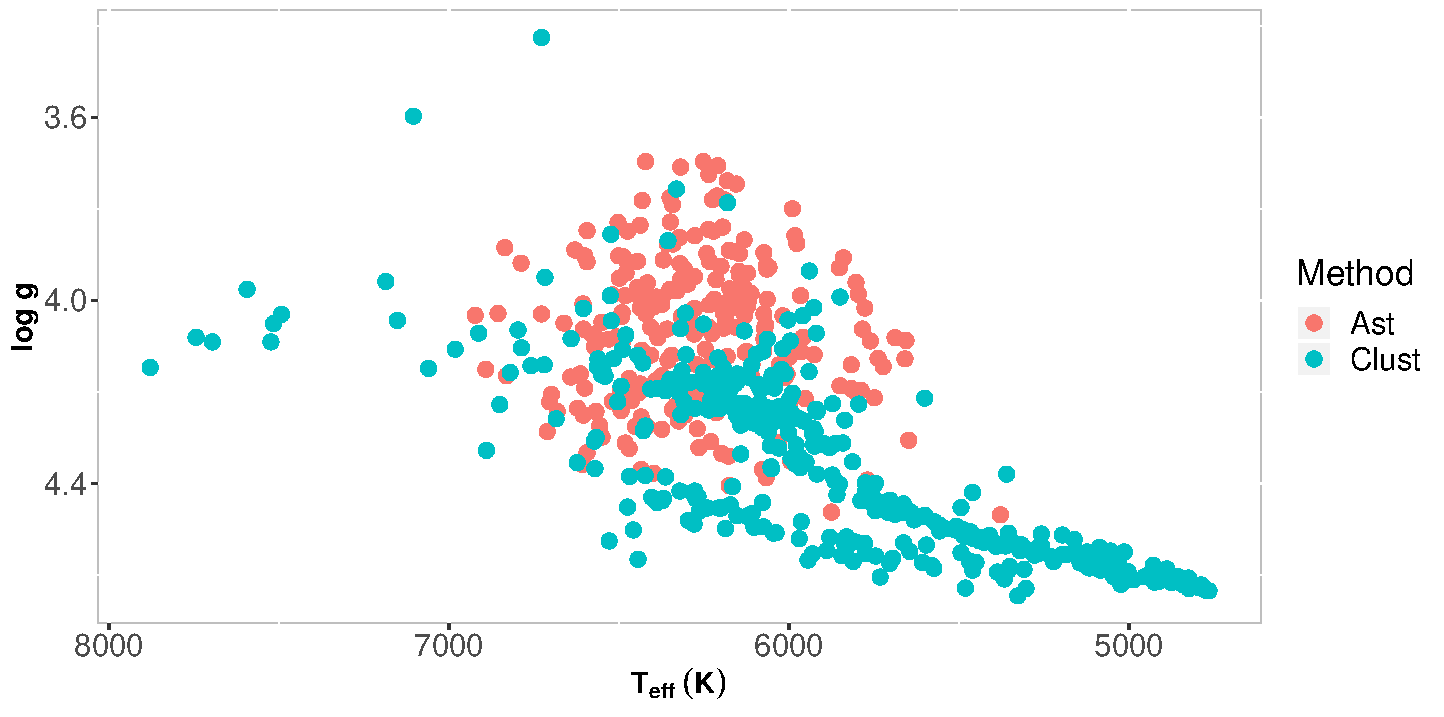
\includegraphics[width=0.9\linewidth]{Figuras/sampling_MS_astro_clust_embedded.pdf}
\end{center}
\caption{Diagrama HR mostrando la muestra MS.}
 \label{Fig:HR_select}
\end{figure}

La idea clásica de la girocronología consiste en estimar las edades estelares utilizando cualquier indicador de la masa estelar y el periodo rotacional estelar. Como se tiene una estimación de masa para toda la muestra de entrenamiento, se puede representar directamente $M$ vs. $P_{\rm rot}$ (Fig. \ref{Fig:M_rot}), evitando usar otros indicadores. En este gráfico, también se diferencian las estrellas astrosísmicas de los cúmulos. No hay diferencias claras entre ellos, excepto el sesgo ya mencionado de la muestra astrosísmica hacia estrellas más masivas. El límite de Kraft está claro alrededor de 1,2M$_\odot$.

\begin{figure}[H]
\begin{center}
 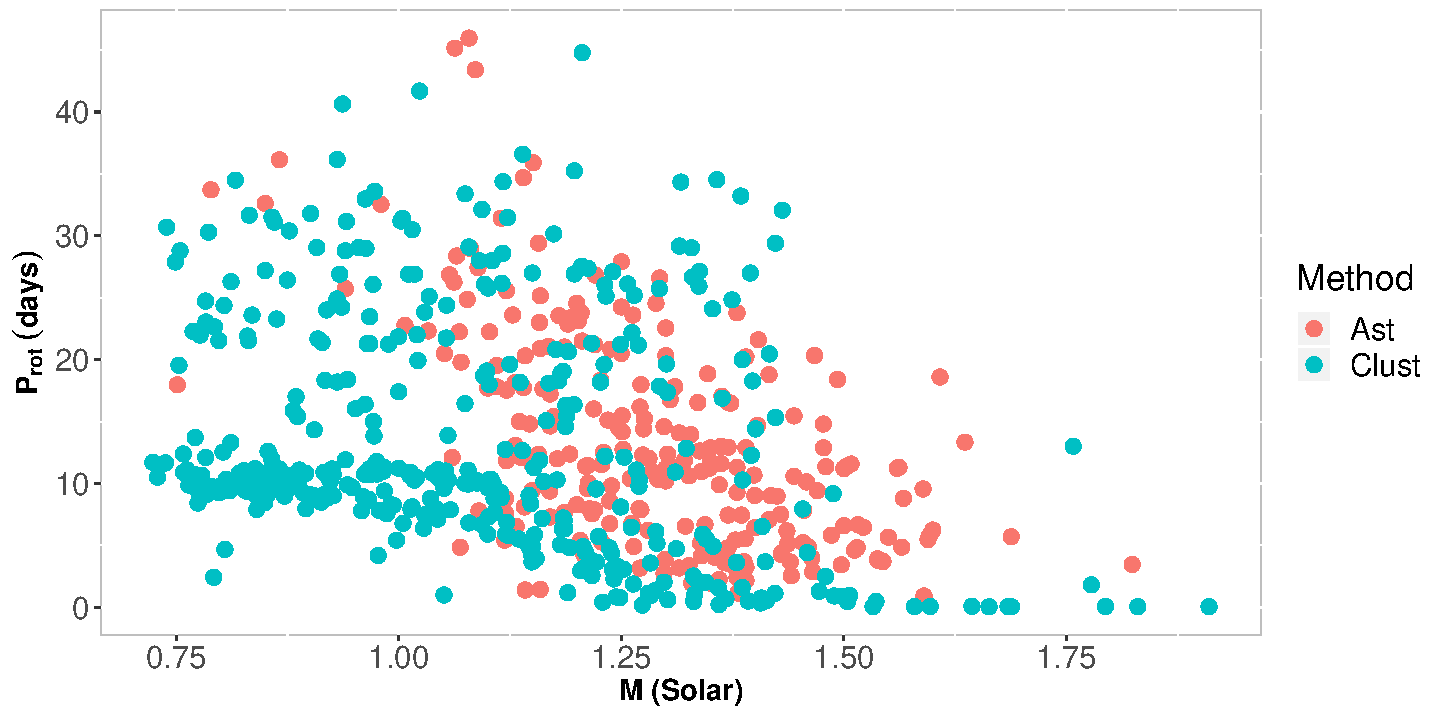
\includegraphics[width=0.9\linewidth]{Figuras/M_Prot_embedded.pdf}
\end{center}
\caption{$M$ - $P_{\rm rot}$ para las estrellas elegidas.}
 \label{Fig:M_rot}
\end{figure}


Si se añade la información de la edad estelar a la gráfica $M$ vs. $P_{\rm rot}$, se obtiene la Figura \ref{Fig:M_Age_rot}. Aquí se puede observar que, con una gran dispersión, cuanto mayor es $P_{\rm rot}$, mayor es la edad. Es destacable que también es cierto para estrellas masivas, por encima del límite de Kraft. Es decir, incluso en ausencia de una envolvente convectiva exterior desarrollada, también se produce la reducción de la velocidad de rotación con el tiempo.

\begin{figure}[H]
\begin{center}
 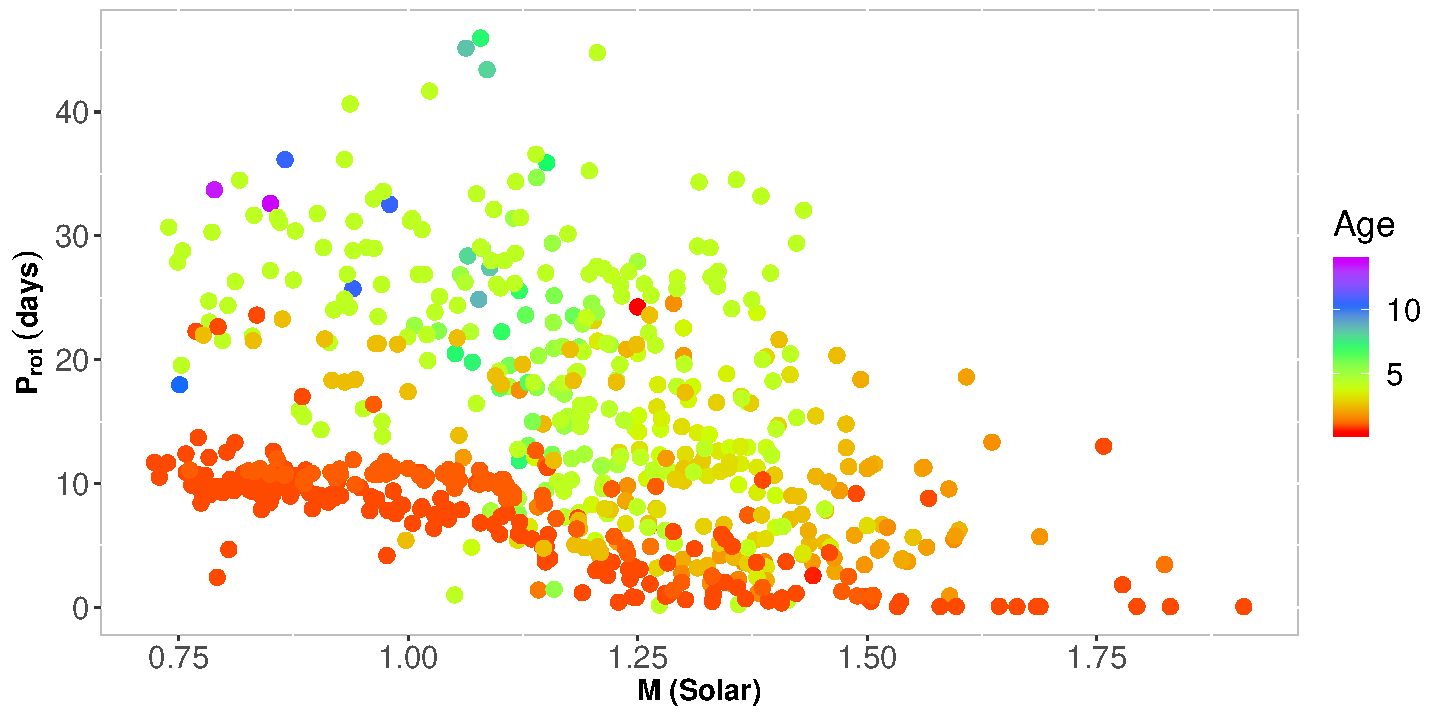
\includegraphics[width=0.8\linewidth]{Figuras/M_Prot_Age_embedded.pdf}
\end{center}
\caption{$M$ - $P_{\rm rot}$ para las estrellas elegidas. La edad se muestra en escala de color.}
 \label{Fig:M_Age_rot}
\end{figure}

Si se representa la edad frente a su periodo de rotación, se obtiene la Figura \ref{Fig:Age_rot}. En general, se confirma que a mayor edad, mayor periodo de rotación, con una gran dispersión, principalmente para estrellas en cúmulos debido a la dependencia de masa del frenado de rotación. También se ha ajustado una regresión lineal a esta relación, diferenciando entre las estrellas astrosísmicas y los cúmulos. Aquí se puede observar uno de los sesgos de la muestra. Estas relaciones lineales tienen la misma tendencia pero apenas son diferentes para cada subgrupo. En cualquier caso, la dispersión es realmente grande y no se puede asegurar que estas regresiones se puedan utilizar para estimar la edad. Esta es la razón por la que se pasa a métodos de análisis basados en Inteligencia Artificial para generar modelos adecuados para estimaciones de edades estelares.

\begin{figure}[H]
\begin{center}
 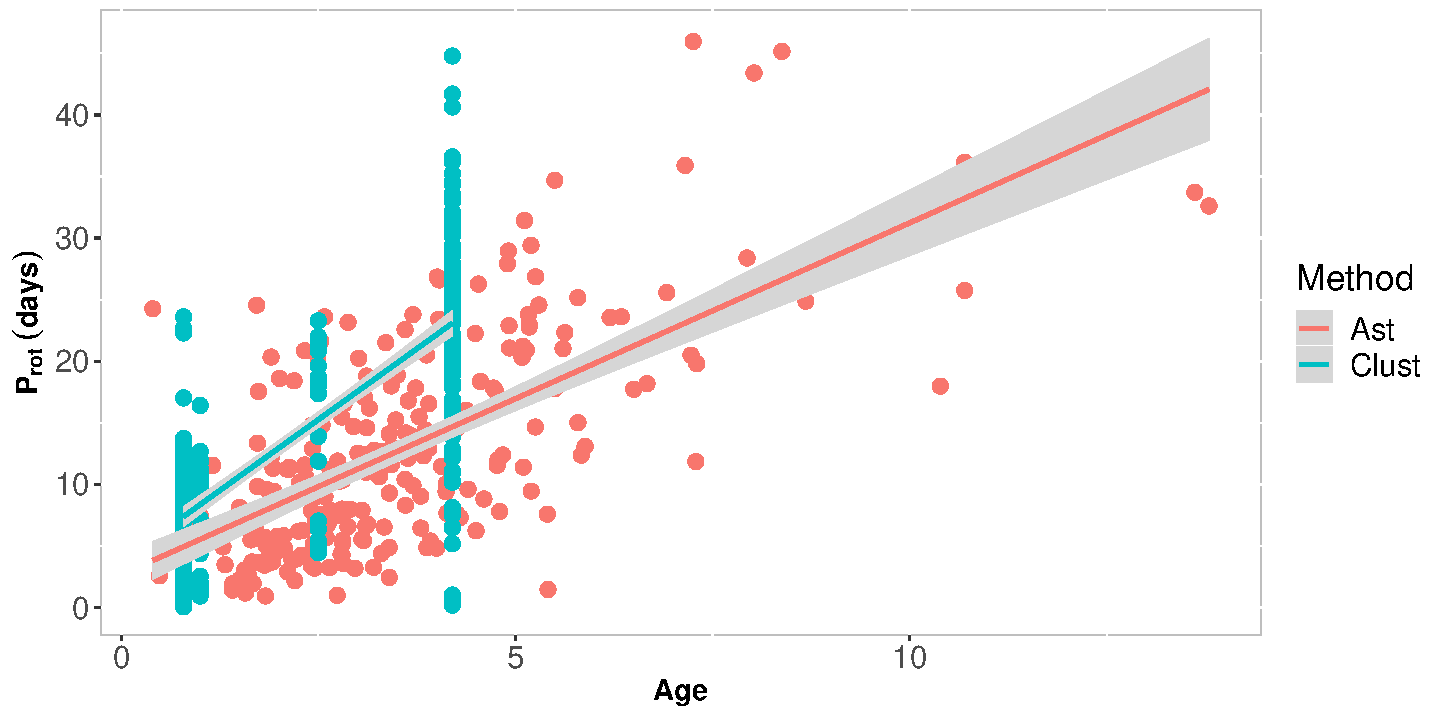
\includegraphics[width=0.8\linewidth]{Figuras/Age_Prot_embedded.pdf}
\end{center}
\caption{$Edad$ - $P_{\rm rot}$ para las estrellas elegidas. Las estrellas asterosísimicas y de cúmulos se muestran en colores diferentes. También se representa la regresión lineal obtenida usando estos dos grupos.}
 \label{Fig:Age_rot}
\end{figure}


\chapter{Modelos y resultados} 

\section{Modelos}
\label{sec:models}

\textbf{Linear regressor} {} Primero se entrena un modelo de datación de estrellas asumiendo que la edad es combinación lineal de las características proporcionadas en la muestra de datos. Sea $\hat{a}$ el valor de la edad predecida, entonces
\begin{equation}
\hat{a}(\vb{w}, \vb{x}) = w_0 + w_1 x_1 + ... + w_D x_D \; ,
\end{equation}
donde $\vb{x}$ y $\vb{w}$ codifican el vector de características de entrada y el coeficiente del regresor lineal, respectivamente. Se sigue el enfoque de mínimos cuadrados para el aprendizaje del modelo, resolviendo un problema de forma: $\min_{\vb{w}} || \vb{X} \vb{w} - \vb{a}||_2^2$. $\vb{X}$. $\vb{X}$ es una matriz que contiene todos los vectores de entrenamiento y $\vb{a}$ es el vector de edades. 

Durante la fase de aprendizaje del modelo, se lleva a cabo una optimización de su hiperparámetro interno \emph{normalize} a través de un proceso de grid search con validación cruzada. De forma predetemrinada se encuentra desactivado, pero al activarlo, los regresores X se normalizan antes de la regresión restando la media y dividiendo por la norma l2.

\vspace{0.5cm}

\textbf{Bayesian Regression} {} Se implementa un regresor Bayessian Ridge para estimar un modelo probabilístico del problema de datación estelar con la forma:
\begin{equation}
p(a|\vb{X},\vb{w},\alpha) = \mathcal{N}(a|\vb{X} \vb{w},\alpha)\; ,
\end{equation}

donde se asume la edad salida $a$ como una distribución gaussiana sobre $\vb{X}\vb{w}$. $\alpha$ se estima directamente a partir de los datos que se tratan como una variable aleatoria. El parámetro de regularización se ajusta a los datos disponibles, introduciendo sobre los hiperparámetros del modelo, \ie $\vb{w}$, el siguiente gaussiano esférico $p(\vb{w}|\lambda) =
\mathcal{N}(\vb{w}|0,\lambda^{-1}\mathbf{I}_{D})$.

Para este regresor, se optimiza con validación cruzada el hiperparámetro asociado al número máximo de iteraciones, que tomará los valores 100, 200, 300, 400, 500.

\vspace{0.5cm}

\textbf{Decision Tree Regressor} {} Se usa un modelo de árbol de decisión \cite{Breiman1984}. Durante el aprendizaje, el modelo optimiza sus hiperparámetros internos a través de un proceso de grid search con validación cruzada. Especificamente, se ajustan: la estrategia par elegir la división en cada nodo del árbol (mejor o aleatorio); el número mínimo de muestras requeridas para estar en un nodo hoja (5, 10, 50, 100); y la función para medir la calidad de la división (error cuadrático medio, error cuadrático medio con la puntuación de mejora de Friedman para posibles divisiones, error medio absoluto con reducción de la desviación de Poisson para encontrar divisiones). 

\vspace{0.5cm}

\textbf{Random Forest Regressor} {} Este modelo de regresión se implementa siguiendo el trabajo de Breiman \cite{Breiman2001}, donde los árboles de decisión se contruyen a partir de las muestras de datos extraídas con reemplazo del conjunto de entrenamiento. De nuevo se usa un proceso de grid search más validación cruzada para ajustar los siguientes hiperparámetros: número de árboles (5, 10, 50, 100); número mínimo de muestras requeridas para estar en un nodo hoja (5, 10, 50, 100); y la función para medir la calidad de la división (error cuadrático medio o error medio absoluto).

\vspace{0.5cm}

\textbf{Support Vector Regression} {} En el estudio se incluye este modelo de regresión, basado en la implementación LibSVM para regresión, \cite{LIBSVM}, siguiendo la aproximación $\epsilon$-SVR. Se emplea el kernel RBF, y se realiza una un grid search con validación cruzada para ajustar el parámetro $C$ (1, 10, 100, 1000).

\vspace{0.5cm}

\textbf{Gaussian Process} {} Se entrena un regresor de proceso gaussiano \cite{Rasmussen2006}, donde se supone que la es constante y cero. Para la covarianza se usa un kernel que es la suma de los siguientes tres kernels. RBF, $k(\vb{x}_i, \vb{x}_j) = \text{exp}\left(- \frac{d(\vb{x}_i, \vb{x}_j)^2}{2l^2} \right)$, donde $d(\cdot, \cdot)$ es la distancia euclídea y $l$ es el parámetro de escala de longitud. Producto escalar, $k(\vb{x}_i, \vb{x}_j) = \sigma_0 ^ 2 + \vb{x}_i \cdot \vb{x}_j$. Es un kernel no estacionario que se obtiene de la regresión lineal poniendo a priori los coeficiones de $x_i (i = 1, \ldots, N)$ y  $N(0, \sigma_0^2)$ para el sesgo. Y finalmente, White kernel, $k(x_i, x_j) = noise\_level \text{ if } x_i == x_j \text{ else } 0$. La aplicación clave del White kernel es parte de un kernel suma, donde describe la componente de ruido de la entrada. Ajustar su parámetro se corresponde con estimar el nivel de ruido en ese momento.

\vspace{0.5cm}

\textbf{k-Nearest Neighbors} {} También se incluye en la comparativa un regresor kNN. Básicamente, se ajusta el parámetro k (1, 5, 10, 15, 20, 50) y el tipo de función de ponderación que se usa para escalar la contribución de cada vecino. Se exploran dos tipos de funciones de ponderación: a) uniforme, donde todos los puntos en cada vecindario se ponderan por igual; y b) distancia, que pondera los puntos por la inversa de su distancia a un punto de consulta.

\vspace{0.5cm}

\textbf{Neural Network} {} La arquitectura implementada se muestra en la figura \ref{fig:neural_network}. Esta consiste en un perceptrón multicapa. El modelo incluye una capa de entrada, un conjunto de 3 capas ocultas fully-connected con 50 unidades en cada una, y la capa de salida encargada de la regresión de las edades de las estrellas. Cada unidad oculta va seguida de una función de activación ReLU. Se usa como función de pérdidas el error cuadrático medio, $Loss(\hat{a},a,W) = \frac{1}{2}||\hat{a} - a ||_2^2 + \frac{\alpha}{2} ||W||_2^2$, donde $W$ codifica los pesos de la red, y $\alpha$ es el parámetro de regularización. La retropropagación \cite{LeCun2012} se utiliza para el aprendizaje del modelo con el optimizador SDG~\cite{sgd}. Durante el aprendizaje, se fija $\alpha=0.01$, y se usa una política de tasa de aprendizaje adaptativa, comenzando con un valor $0.1$.

\vspace{0.5cm}

\begin{figure}[H]
\begin{center}
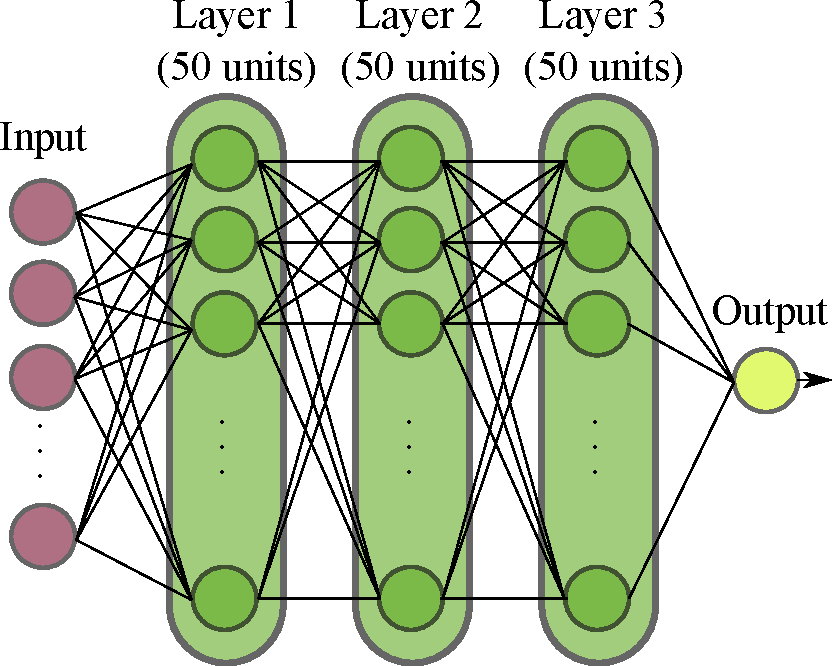
\includegraphics[width=0.6\linewidth]{Figuras/nnet.pdf}
\end{center}
\caption{Arquitectura de la red neuronal implementada. Se han usado 3 capas ocultas, con 50 unidades en cada una seguida de una ReLU. La salida no tiene función de activación, para realizar directamente la estimación de la edad.}
\label{fig:neural_network}
\end{figure}

\textbf{Stacking} {} Finalmente, se emplea un método de ensamblado en machine learning conocido como generalización apilada o stacking \cite{Wolpert1992}. En un problema de regresión como lo es este, las predicciones de cada regresor individual (nivel 0) se apilan y se introducen en un estimador final (nivel 1), que calcula la predicción de la edad. Para este proyecto, en el nivel 0, se integran: Neural Network y Gaussian Process. Para la última capa (nivel 1), se incorpora un Linear Regressor. Durante el entrenamiento, y para generalizar y evitar sobreajuste, el estimador de nivel 1 se entrena con muestras externas (tomadas del conjunto de entrenamiento), siguiendo una metodología de validación cruzada.

\section{Benchmark}
\label{sec:benchmark}

La muestra de datos, detallada en la Sección \ref{sec:data}, ofrece más de 600 estrellas, con edades precisas, donde se propone construir los siguientes escenarios de evaluación.

\vspace{0.5cm}

\textbf{Problema de datación estelar (Benchmark A)} {} En esta configuración, se propone evaluar los diferentes modelos de regresión siguiendo un esquema clásico de división de datos de entrenamiento/prueba. A partir de la distribución de la muestra de datos, se define un conjunto de entrenamiento y un conjunto de pruebas, donde el  80 \% y el 20 \% de las estrellas se han incluido al azar, respectivamente. En la Figura \ref{fig:benchA_train} se detalla la distribución de las estrellas en el conjunto de entrenamiento y en la Figura \ref{fig:benchA_test} la del conjunto de prueba.

\begin{figure}[H]
\begin{center}
 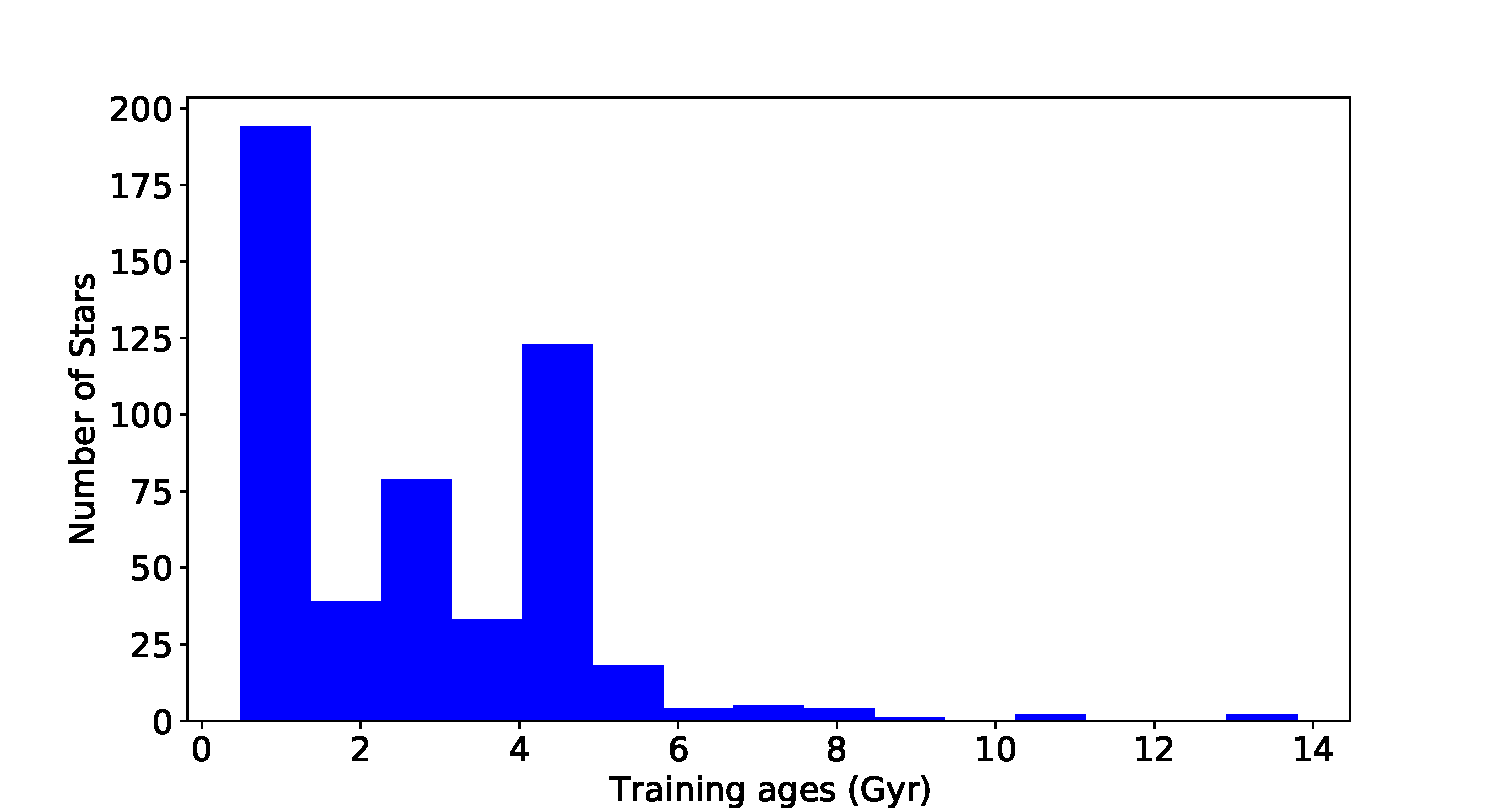
\includegraphics[width=0.8\linewidth]{Figuras/Experimentos/B_A_training.pdf}
\end{center}
\caption{Benchmark A: Distribución de las estrellas que forman el subconjunto de entrenamiento.}
 \label{fig:benchA_train}
\end{figure}

\begin{figure}[H]
\begin{center}
 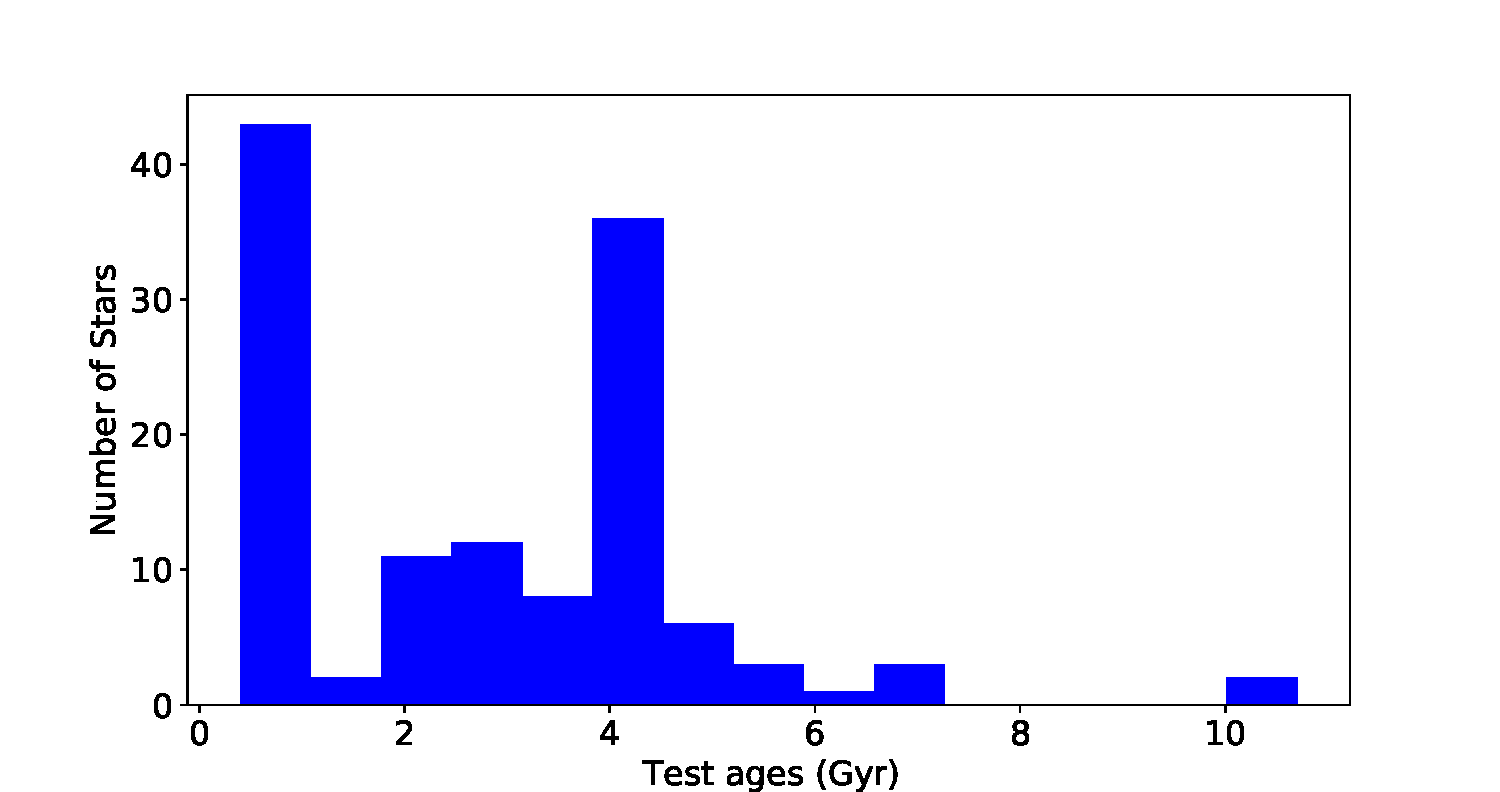
\includegraphics[width=0.8\linewidth]{Figuras/Experimentos/B_A_test.pdf}
\end{center}
\caption{Benchmark A: Distribución de las estrellas que forman el subconjunto de prueba.}
 \label{fig:benchA_test}
\end{figure}


\textbf{Capacidad de generalización (Benchmark B)} {} En primer lugar, se proporciona un estudio de generalización para los modelos, donde se entrena con un enfoque de estrellas \emph{jóvenes}, y se evalúa su rendimiento en estrellas \emph{ancianas}. Este escenario, denominado Benchmark B1, es interesante para evaluar la capacidad de los modelos de Inteligencia Artificial para trabajar con estrellas cuyo rango está fuera del conjunto de entrenamiento. Los rangos de edad de entrenamiento y prueba son $[0.4,4.2]$ y $[4.2,13.8]$ Gyr, respectivamente. En la Figura \ref{fig:benchB1_train} se detalla la distribución de las estrellas en el conjunto de entrenamiento y en la Figura \ref{fig:benchB1_test} la del conjunto de prueba.

\begin{figure}[H]
\begin{center}
 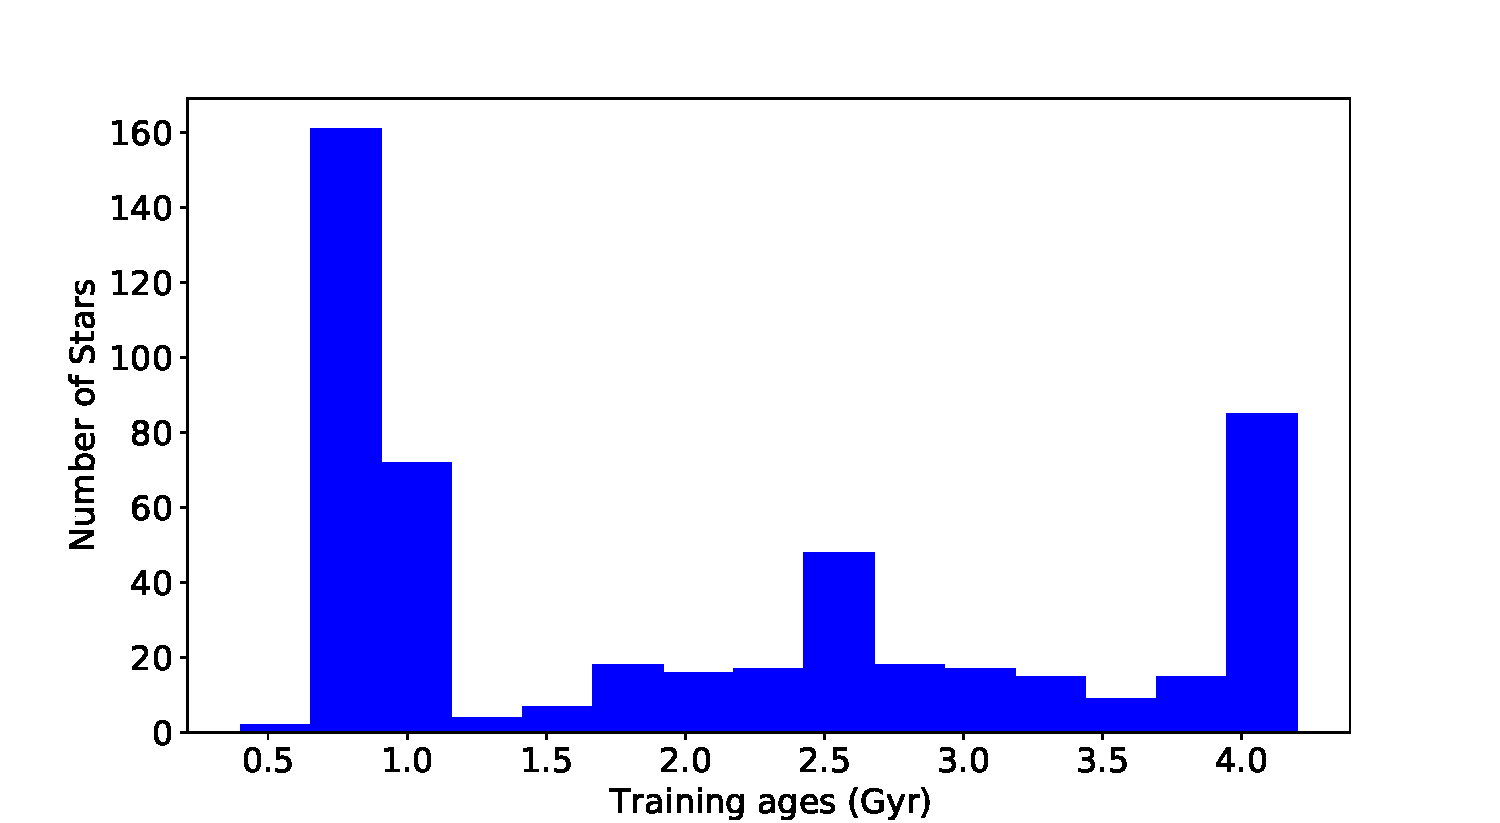
\includegraphics[width=0.8\linewidth]{Figuras/Experimentos/B_B1_training.pdf}
\end{center}
\caption{Benchmark B1: Distribución de las estrellas que forman el subconjunto de entrenamiento.}
 \label{fig:benchB1_train}
\end{figure}

\begin{figure}[H]
\begin{center}
 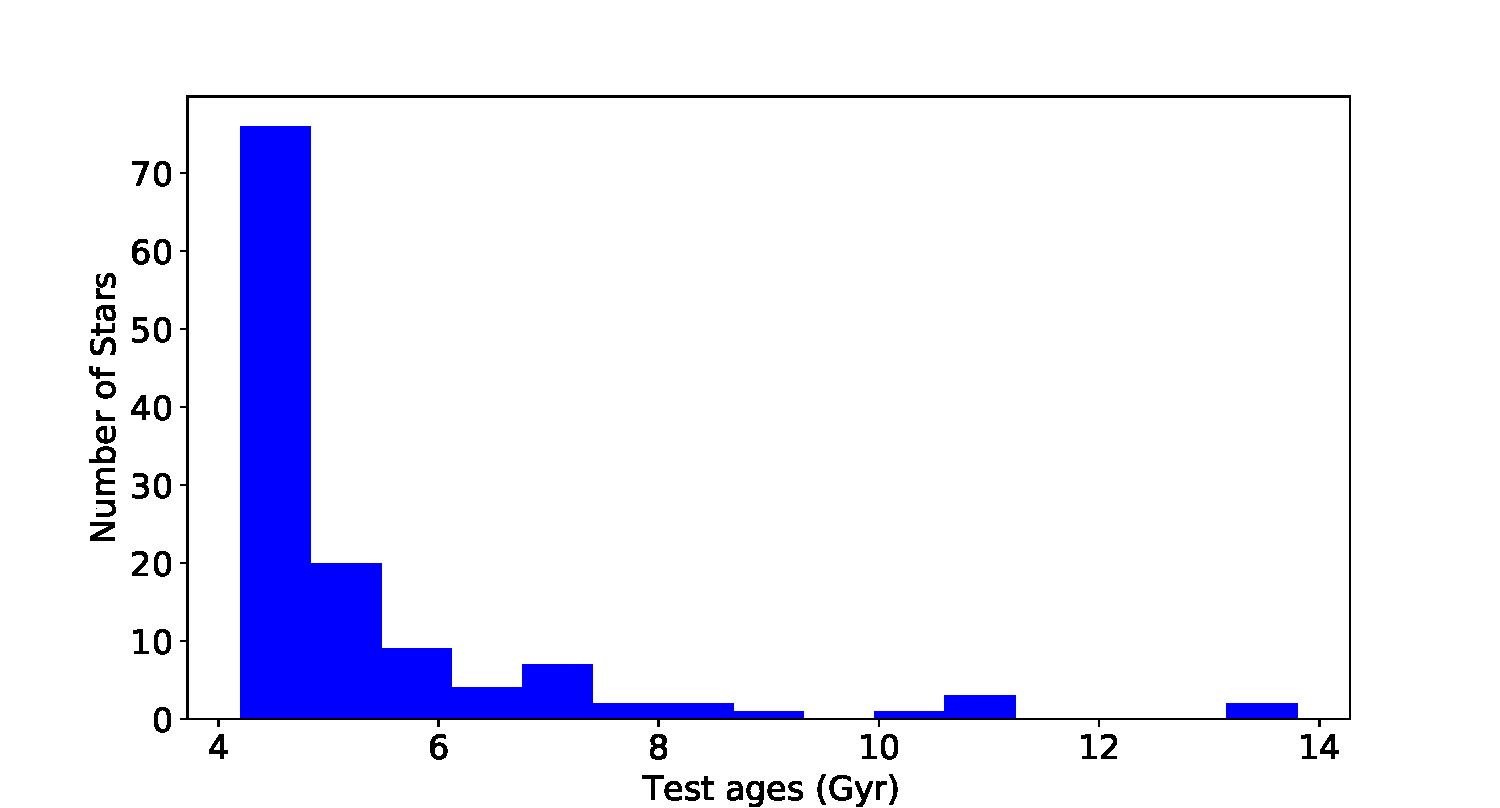
\includegraphics[width=0.8\linewidth]{Figuras/Experimentos/B_B1_test.pdf}
\end{center}
\caption{Benchmark B1: Distribución de las estrellas que forman el subconjunto de prueba.}
 \label{fig:benchB1_test}
\end{figure}

También se propone un segundo escenario para evaluar la capacidad de generalización de los modelos cuando se entrenan solo con estrellas pertenecientes a cúmulos. En la práctica, la girocronología se utiliza para datar estrellas individuales que pueden tener cualquier edad. Las estrellas de los cúmulos suelen estar datadas gracias a su pertenencia a los propios cúmulos. En este Benchmark B2, se propone el entrenamiento de los modelos utilizando únicamente estrellas pertenecientes a cúmulos. El resto de estrellas se incluyen en el conjunto de prueba. En total, este escenario recoge 397 y 240 muestras para entrenamiento y prueba, respectivamente. En la Figura \ref{fig:benchB2_train} se detalla la distribución de las estrellas en el conjunto de entrenamiento y en la Figura \ref{fig:benchB2_test} la del conjunto de prueba.

\begin{figure}[H]
\begin{center}
 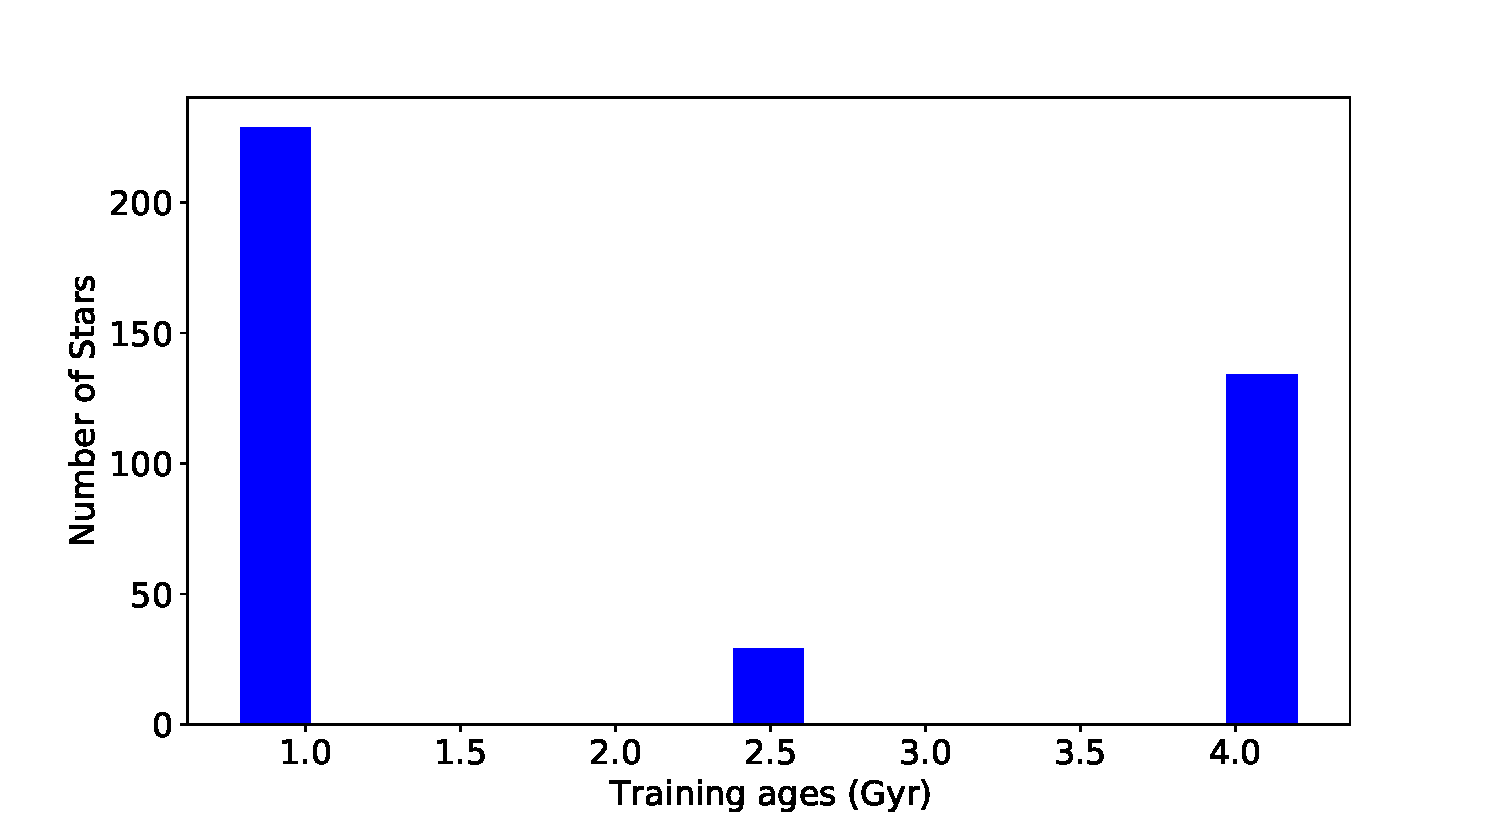
\includegraphics[width=0.8\linewidth]{Figuras/Experimentos/B_B2_training.pdf}
\end{center}
\caption{Benchmark B2: Distribución de las estrellas que forman el subconjunto de entrenamiento.}
 \label{fig:benchB2_train}
\end{figure}

\begin{figure}[H]
\begin{center}
 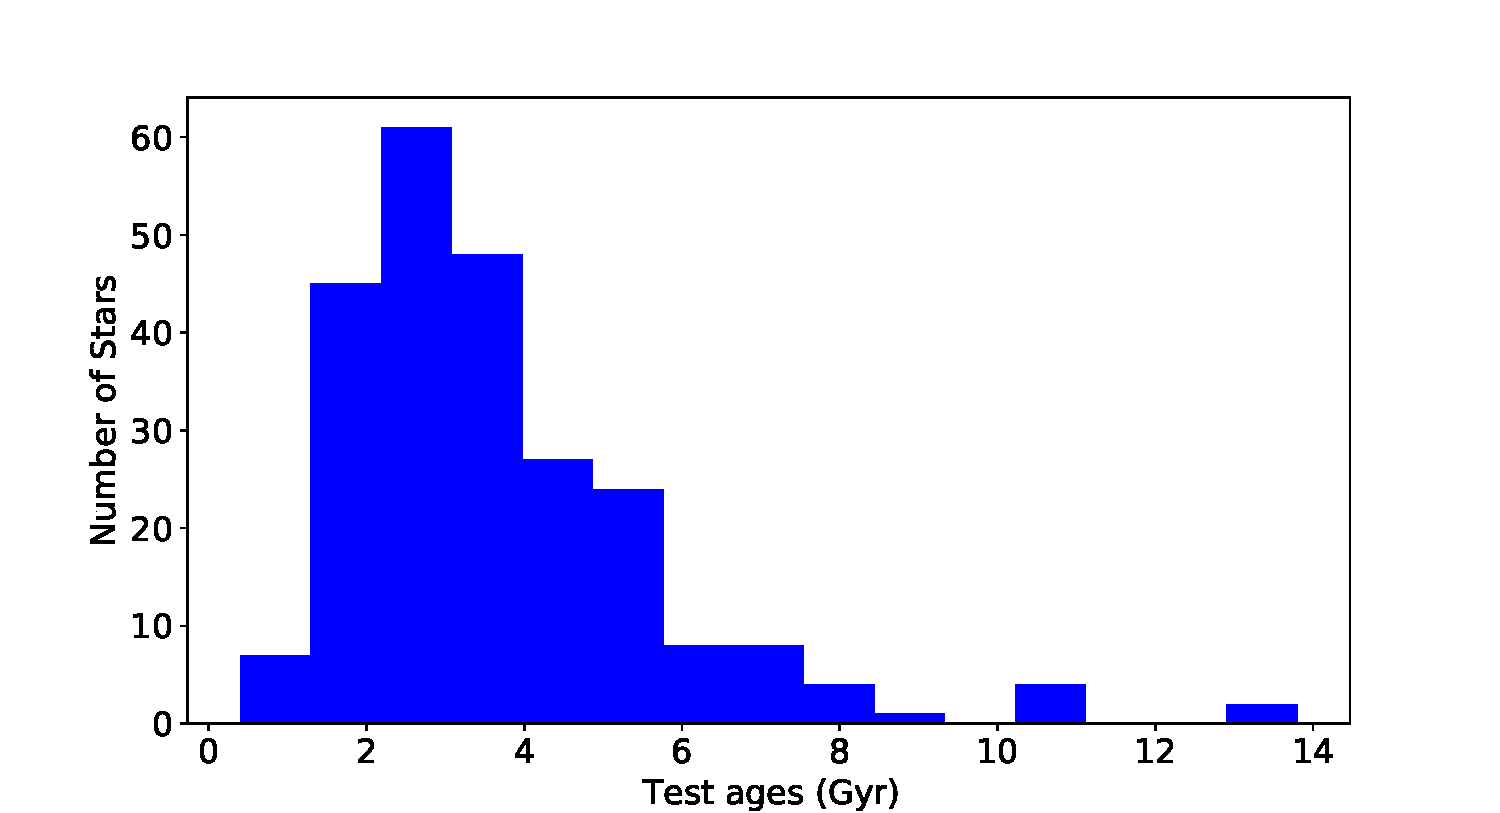
\includegraphics[width=0.8\linewidth]{Figuras/Experimentos/B_B2_test.pdf}
\end{center}
\caption{Benchmark B2: Distribución de las estrellas que forman el subconjunto de prueba.}
 \label{fig:benchB2_test}
\end{figure}

\textbf{Regresión para datación estelar sobre una muestra de control (Benchmark C)} {} Aquí se propone examinar el rendimiento de todos los modelos sobre una muestra de datos de control compuesta por estrellas que no pertenecen a ningún cúmulo, y con una distribución más realista. Especificamente, en este Benchmark C, se evalúan los modelos entrenados con toda la muestra de datos sobre un conjunto de $32$ estrellas nuevas no pertenecientes a cúmulos, incluyendo al Sol. Este conjunto independiente de control se ha obtenido de las mismas fuentes basadas en astrisismología utilizadas para recopilar la información de la muestra descrita en la Sección \ref{sec:data}. Se han reservado 32 estrellas de estas fuentes, antes de contruir la muestra. El rango de edad de este conjunto va de 1,2 a 10,1 Gyr. Este rango se superpone con el rango de edad utilizado en la muestra de entrenamiento ($[0.4, 13.8]$ Gyr), e incluye algunas edades nuevas no observadas. Se presta especial atención a la precisión de los modelos para la estimación de la edad del Sol (4.6 Gyr). En la Figura \ref{fig:benchC_train} se detalla la distribución de las estrellas en el conjunto de entrenamiento y en la Figura \ref{fig:benchC_test} la del conjunto de prueba.

\begin{figure}[H]
\begin{center}
 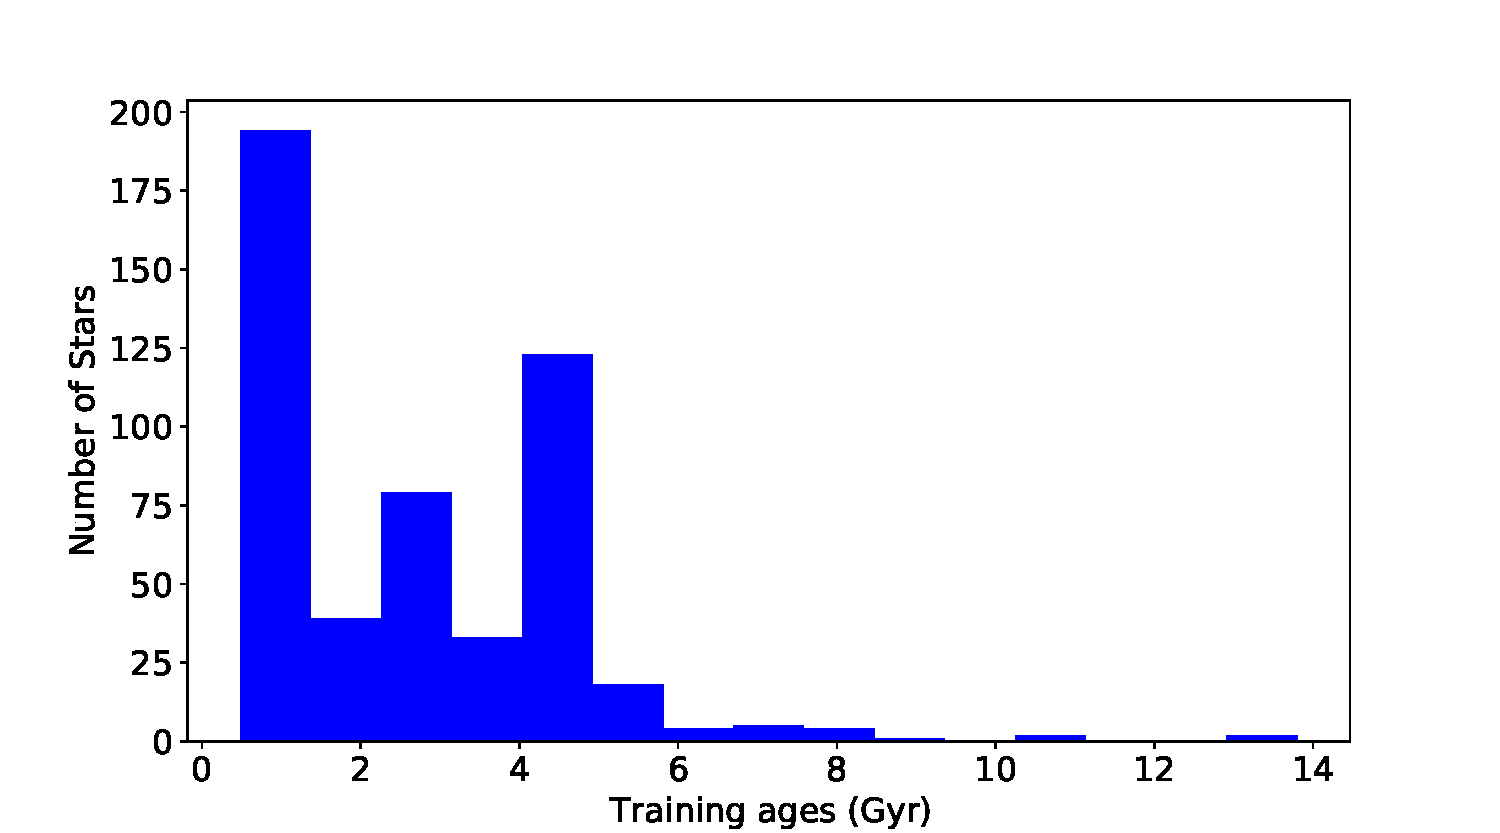
\includegraphics[width=0.8\linewidth]{Figuras/Experimentos/B_C_training.pdf}
\end{center}
\caption{Benchmark C: Distribución de las estrellas que forman el subconjunto de entrenamiento.}
 \label{fig:benchC_train}
\end{figure}

\begin{figure}[H]
\begin{center}
 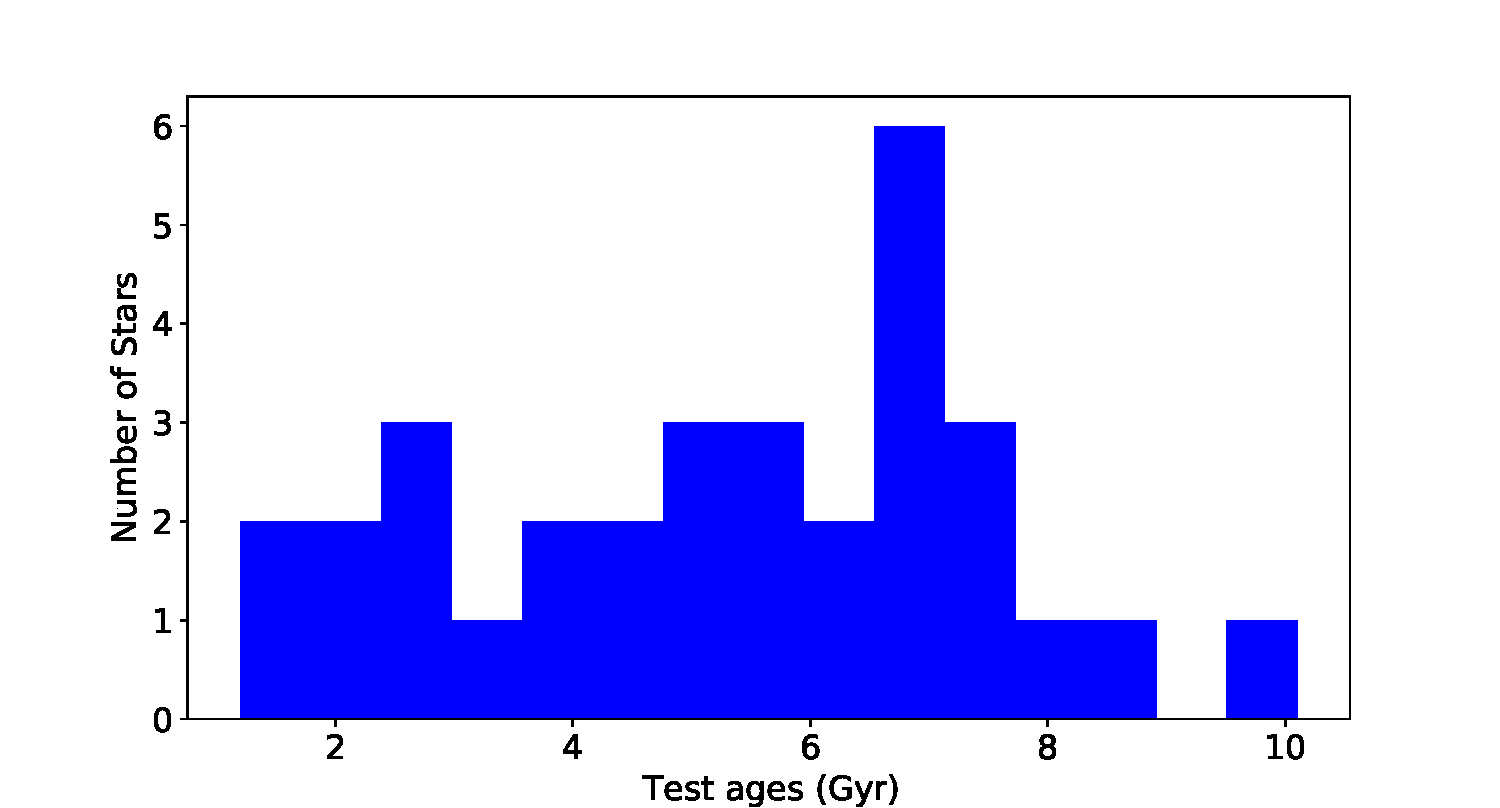
\includegraphics[width=0.8\linewidth]{Figuras/Experimentos/B_C_test.pdf}
\end{center}
\caption{Benchmark C: Distribución de las estrellas que forman el subconjunto de prueba.}
 \label{fig:benchC_test}
\end{figure}


\section{Resultados}
\label{sec:results}
A contnuación, se presenta la configuración experimental y se informa de los resultados obtenidos en la evaluación de los modelos detallados en la Sección \ref{sec:models}. Este benchmarking se realiza a traves de los 3 escenarios descritos: el efecto de los diferentes modelos (Benchmark A); la capacidad de generalización (Benchmark B); y el rendimiento sobre una muestra de control (Benchmark C).

\subsection{Configuración experimental}

\paragraph{Implementación} 
Para poder realizar una comparación entre modelos, se han creado todos en Python, usando la librería scikit-learn \cite{scikit-learn}. Se utilizan las siguientes siglas para identificar los modelos implementados: Neural Network (nnet), Linear Regressor (lr), Decision Tree Regressor (dtr), Random Forest Regressor (rf), Support Vector Regression (svm), Bayesian Regression (bayes), k-Nearest Neighbors (kNN), Gaussian Process (gp) y Stacking (stacking).

\paragraph{Métricas de evaluación}
La métrica de evaluación principal utilizada es el error medio absoluto, $MAE = \frac{\sum_{i=1}^{N}|a_i-\hat{a}_i|}{N}$, donde $a_i$ y $\hat{a}_i$, son la edad proporcionada por el conjunto de datos y la edad estimada por un modelo de regresión, respectivamente. Dado que el conjunto de datos proporciona información sobre la precisión de la edad de cada estrella, en forma de límites de error, también se propone utilizar como métrica de evaluación de la precisión el porcentaje de predicciones de la edad de las estrellas que se encuentran dentro del intervalo de confianza proporcionado por el propio conjunto de datos.

\paragraph{Gráficas}
Antes de abordar cada uno de los benchmarks, es necesario introducir brevemente las gráficas que permiten profundizar en el renidmiento de los modelos. En primer lugar, se muestra un gráfico de barras que recoge un resumen con el MAE de cada uno de los modelos. A continuación y para cada uno de los modelos, se observan 3 gráficas diferentes. La primera de las gráficas permite observar las estimaciones que caen dentro del margen de error. La segunda gráfica muestra detalladamente la predicción, incluyendo el error obtenido para cada uno de los casos. La tercera gráfica muestra un histograma que recoge el MAE en función de la edad de las estrellas del conjunto de prueba.

\subsection{Benchmark A: Problema de datación estelar}

La Figura \ref{fig:benchA_models} muestra el rendimiento de todos los modelos, comparando su MAE correspondiente. En este escenario es interesante de observar que se tienen 2 modelos, más su Stacking, que presentan los mejores resultado, estableciendo un margen de rendimiento con respecto a los demás. Son la Red Neuronal y el Proceso Gaussiano. Su Stacking reduce ligeramente el mejor MAE de la Red Neuronal de 0,405 a 0,400.

Analizando los 6 modelos restantes, se observa que, la mayoría de los modelos presentan dificultades en la estimación de la edad de las estrellas más viejas. También es relevante el resultado proporcionado por un modelo tan simple como un kNN (ver Figura \ref{fig:benchA_details_knn_1} y Figura \ref{fig:benchA_details_knn_2}), con un MAE de solo 0.53 Gyr. El éxito de este modelo se explica mediante los cúmulos que forman la base de datos, donde se encuentran muchos elementos concentrados en 2 valores de edad muy específicos, lo que permite que modelos como kNN hagan estimaciones muy precisas sobre las estrellas de prueba con estas edades. Este hecho se corrobora en la Tabla \ref{table:precisions}, donde se observa que la mejor precisión la logra el modelo kNN, seguido por la Red Neuronal. En general, a excepción de lr y bayes, todos los modelos ofrecen un MAE por debajo de 0.7 Gyr, lo que supone un gran avance en el campo de la datación estelar.

\begin{figure}[H]
\begin{center}
 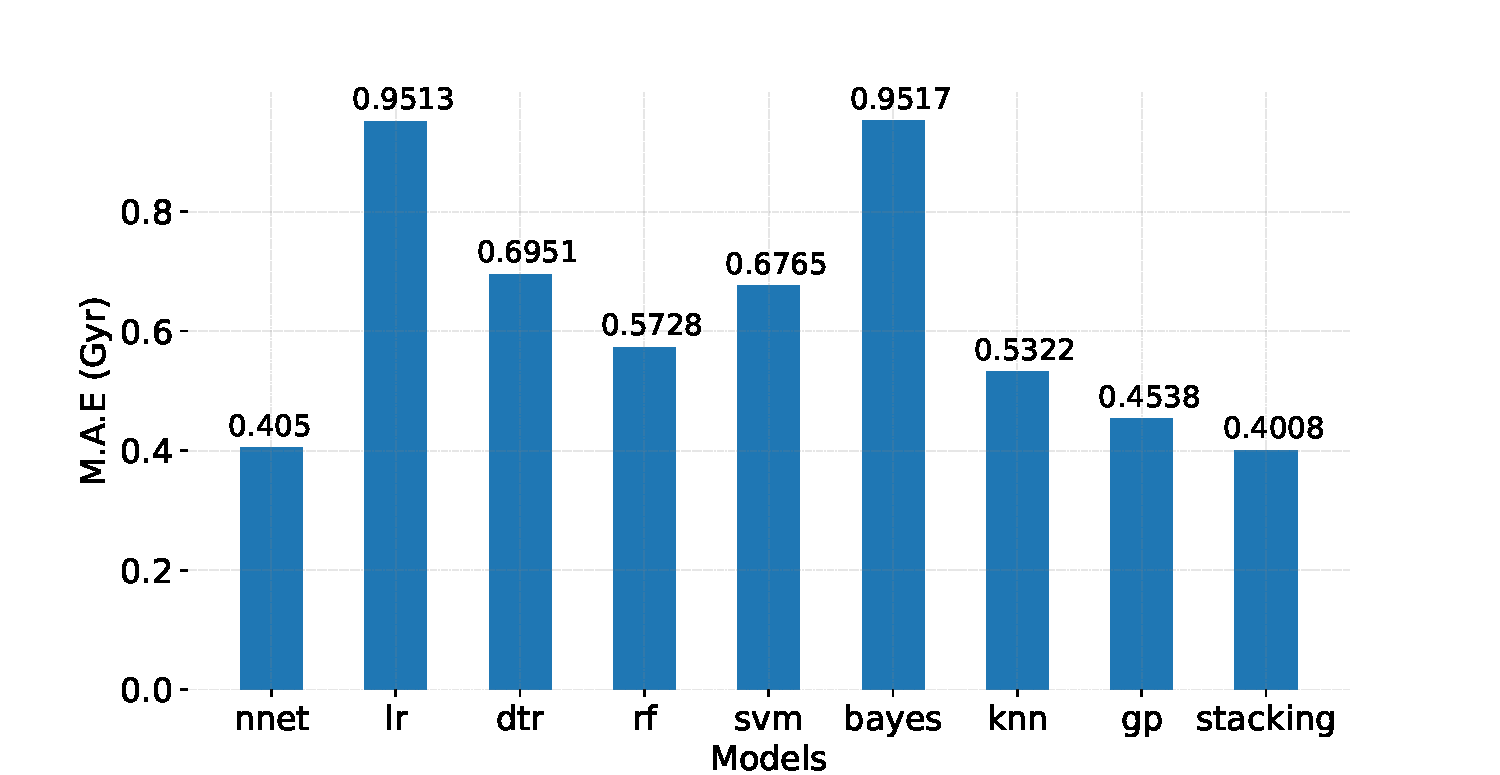
\includegraphics[width=0.8\linewidth]{Figuras/Experimentos/B_A_models.pdf}
\end{center}
\caption{Benchmark A: Rendimiento de los modelos en función del MAE. En esta configuración, las dos mejores aproximaciones son Neural Network (nnet) y Gaussian Process (gp), y por lo tanto, su Stacking.}
 \label{fig:benchA_models}
\end{figure}

\paragraph{Stacking} 
A continuación, se muestran las 3 gráficas que detallan el rendimiento del modelo Stacking, el cual ha presentado el menor MAE en este benchmark, 0.400 Gyr.

\begin{figure}[H]
\begin{center}
 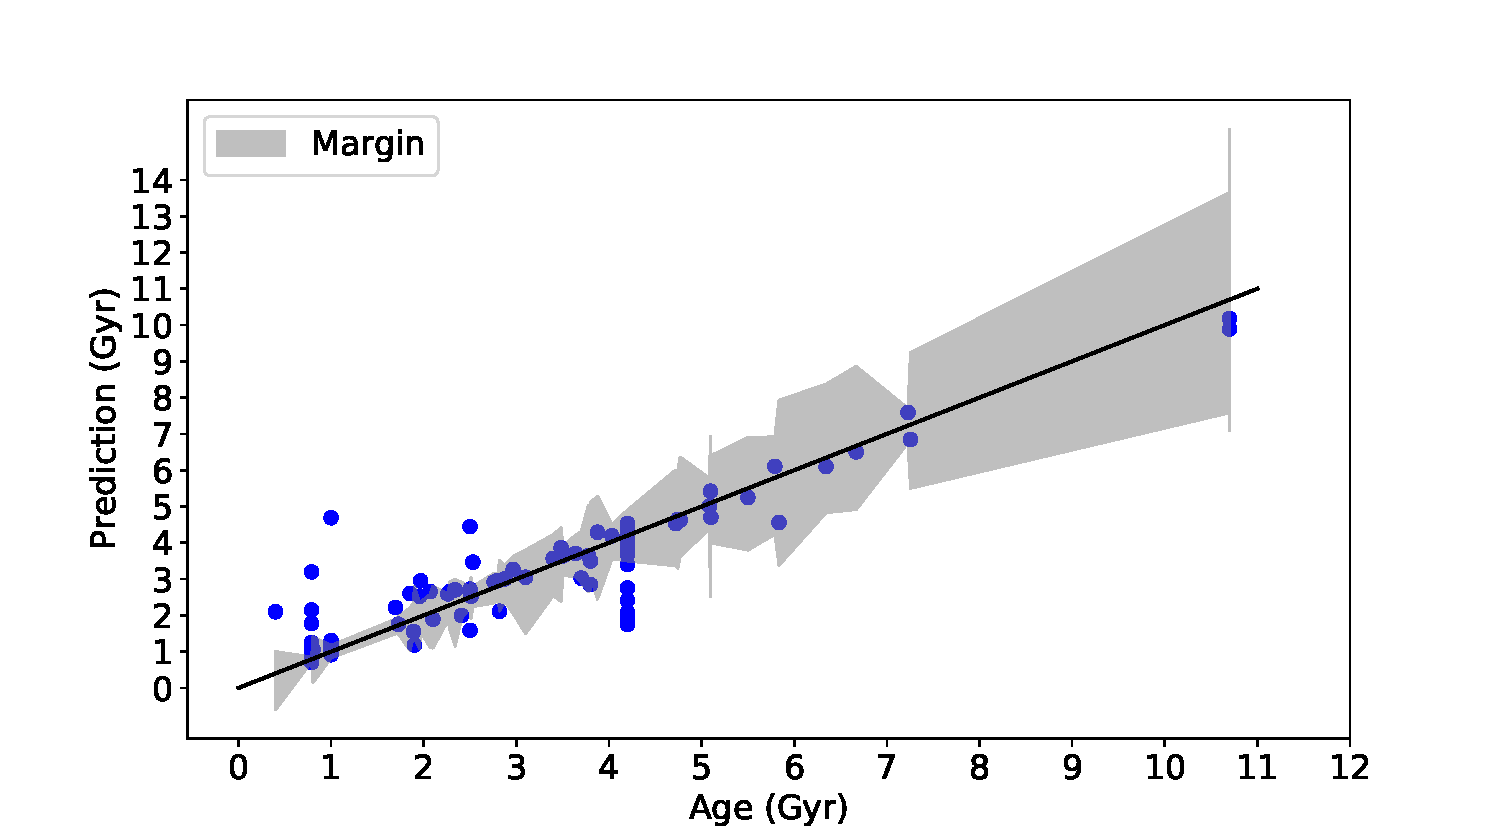
\includegraphics[width=0.8\linewidth]{Figuras/Experimentos/B_A_stacking_1.pdf}
\end{center}
\caption{Benchmark A: Rendimiento para el modelo Stacking.}
 \label{fig:benchA_details_stacking_1}
\end{figure}

\begin{figure}[H]
\begin{center}
 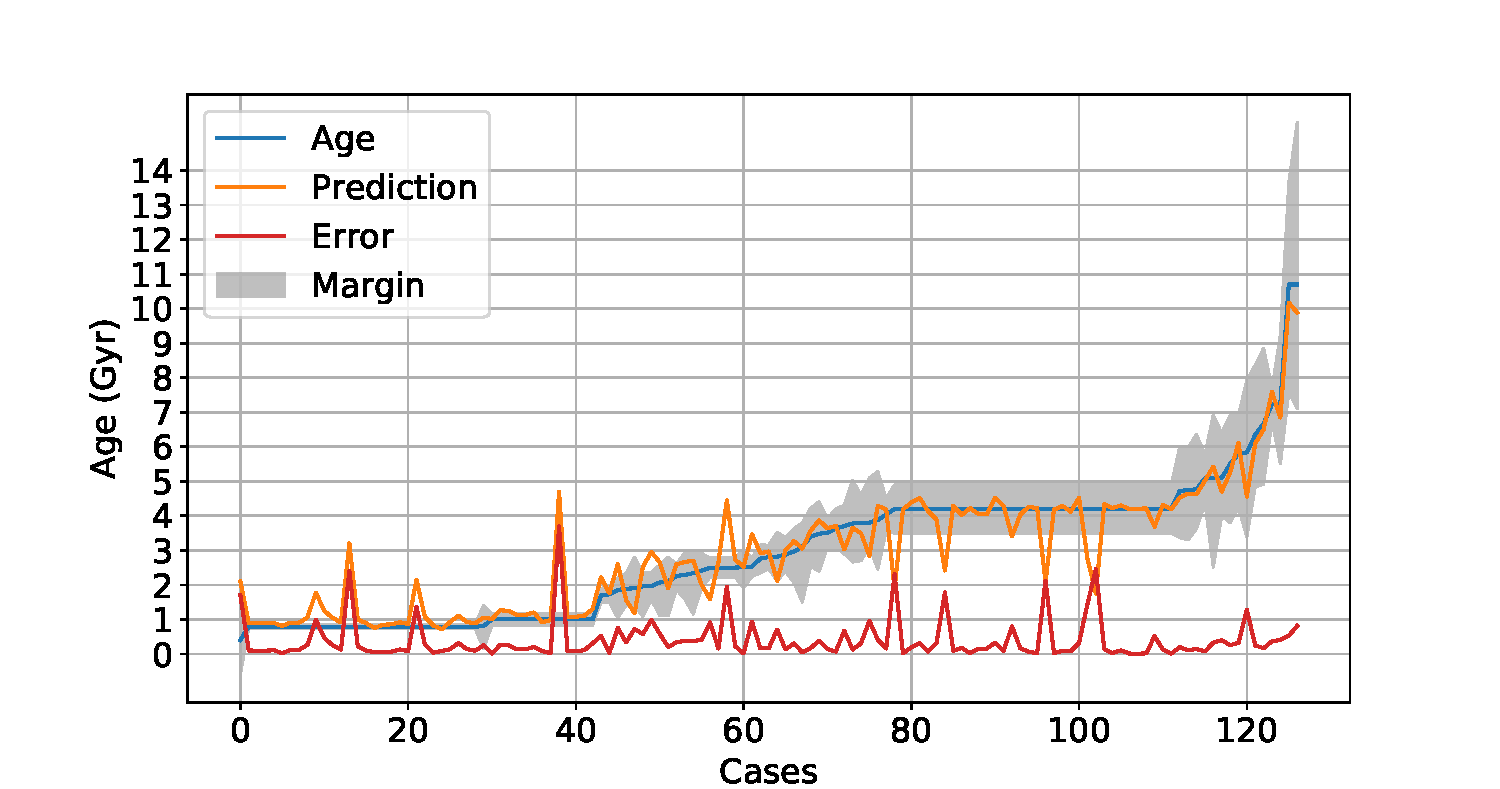
\includegraphics[width=0.8\linewidth]{Figuras/Experimentos/B_A_stacking_2.pdf}
\end{center}
\caption{Benchmark A: Predicción detallada para el modelo de Stacking. Se observa la edad real (en azul), la predicción de los modelos (en naranja), y el error correspondiente (en rojo).}
 \label{fig:benchA_details_stacking_2}
\end{figure}

\begin{figure}[H]
\begin{center}
 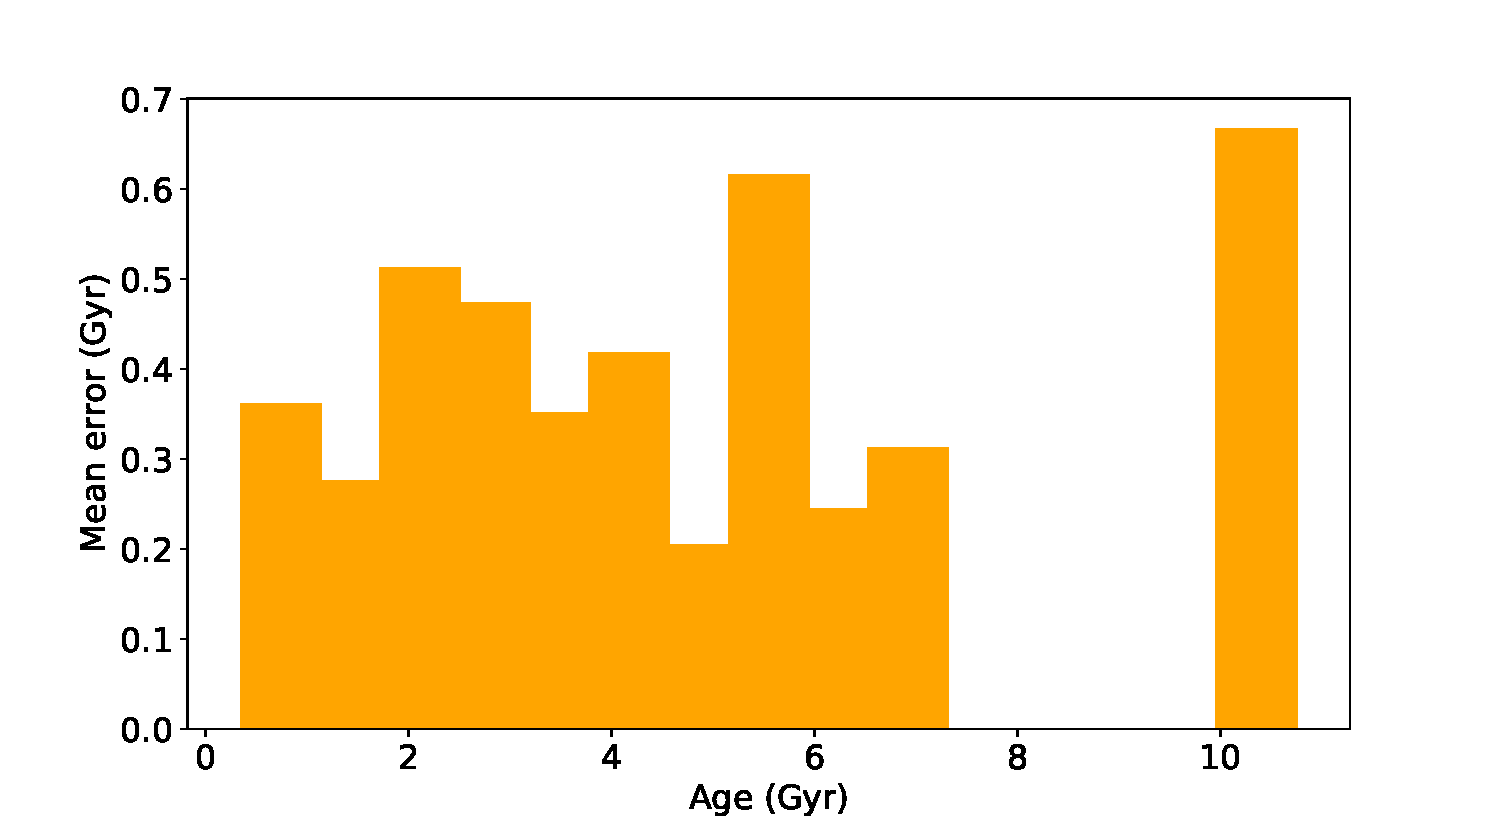
\includegraphics[width=0.8\linewidth]{Figuras/Experimentos/B_A_stacking_3.pdf}
\end{center}
\caption{Benchmark A: MAE en función del rango de edad del conjunto de prueba.}
 \label{fig:benchA_details_stacking_3}
\end{figure}

\paragraph{Neural Network} 
A continuación, se muestran las 3 gráficas que detallan el rendimiento del modelo Neural Network. Segundo mejor modelo con un MAE de 0.405 Gyr.

\begin{figure}[H]
\begin{center}
 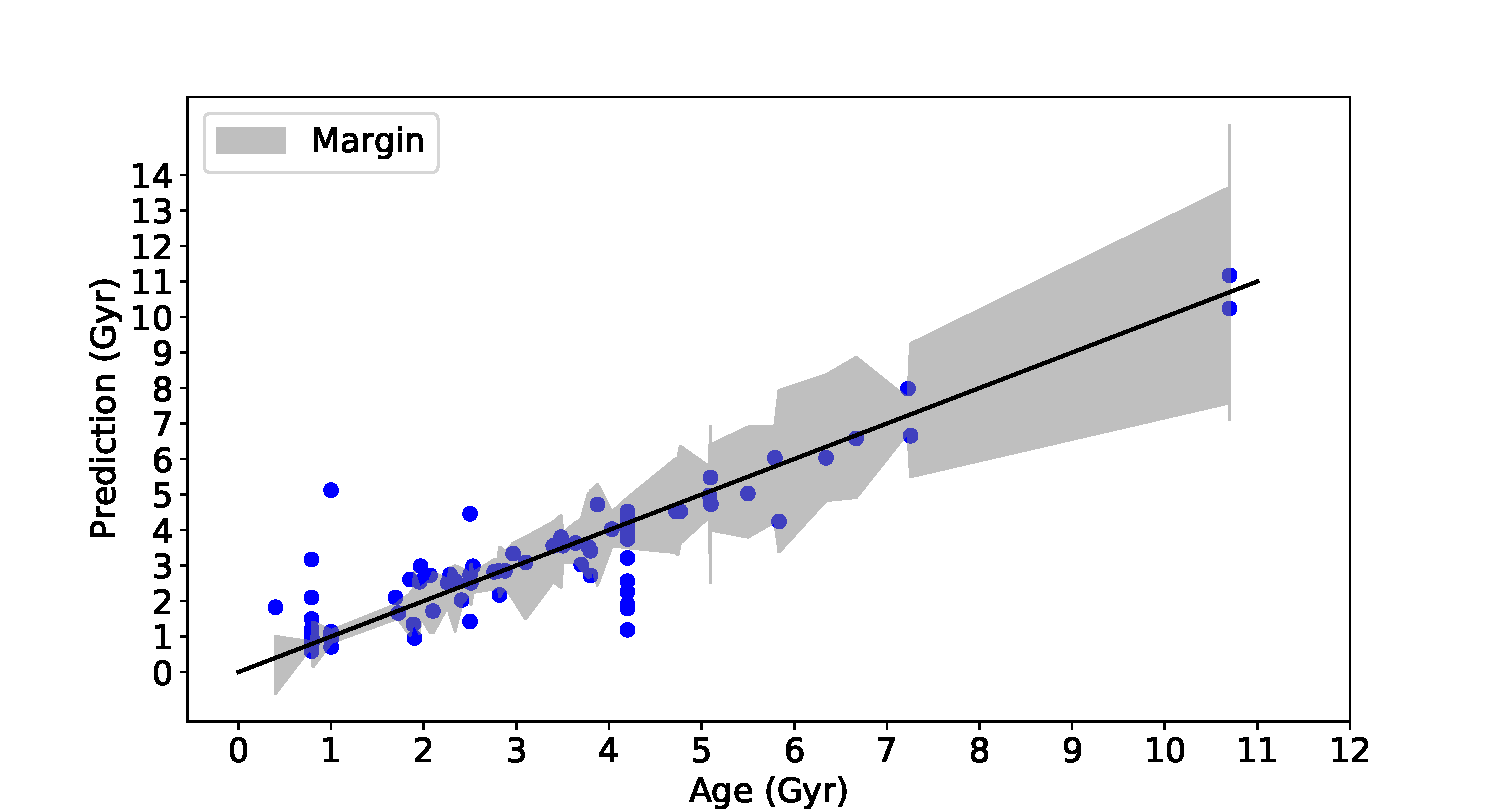
\includegraphics[width=0.8\linewidth]{Figuras/Experimentos/B_A_nnet_1.pdf}
\end{center}
\caption{Benchmark A: Rendimiento para el modelo Neural Network.}
 \label{fig:benchA_details_nnet_1}
\end{figure}

\begin{figure}[H]
\begin{center}
 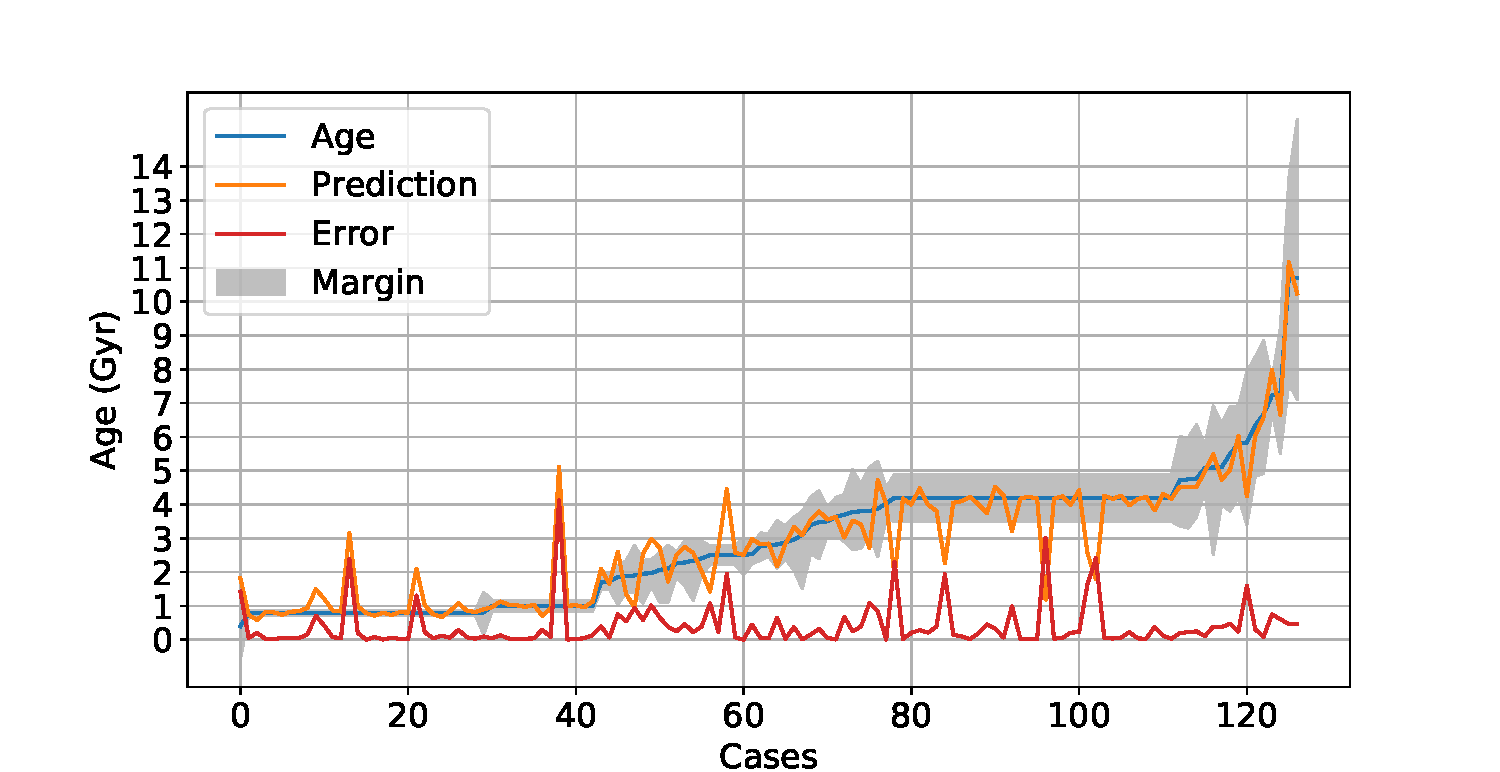
\includegraphics[width=0.8\linewidth]{Figuras/Experimentos/B_A_nnet_2.pdf}
\end{center}
\caption{Benchmark A: Predicción detallada para el modelo de Neural Network. Se observa la edad real (en azul), la predicción de los modelos (en naranja), y el error correspondiente (en rojo).}
 \label{fig:benchA_details_nnet_2}
\end{figure}

\begin{figure}[H]
\begin{center}
 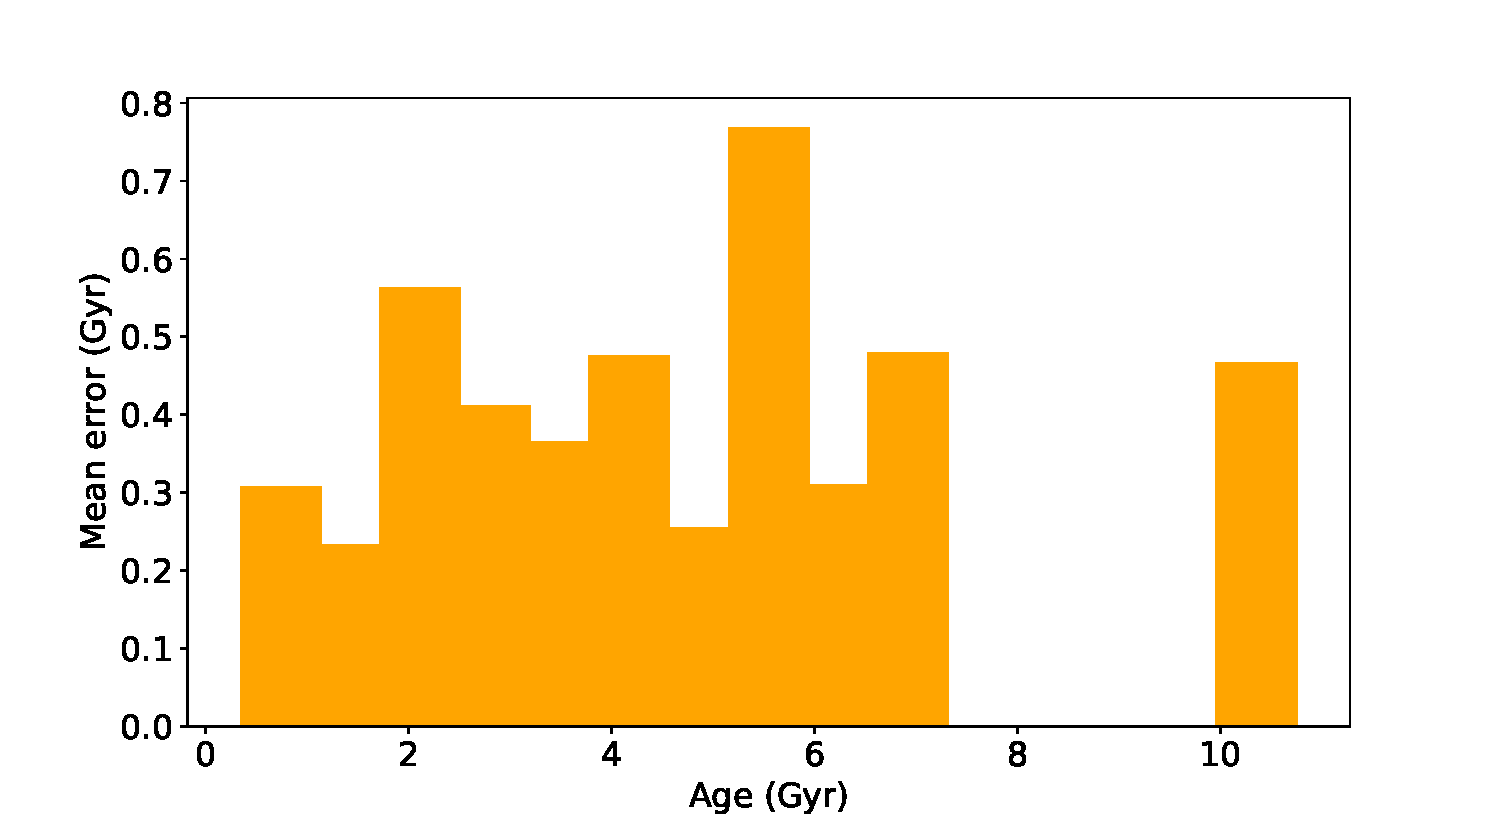
\includegraphics[width=0.8\linewidth]{Figuras/Experimentos/B_A_nnet_3.pdf}
\end{center}
\caption{Benchmark A: MAE en función del rango de edad del conjunto de prueba.}
 \label{fig:benchA_details_nnet_3}
\end{figure}

\paragraph{Gaussian Process} 
A continuación, se muestran las 3 gráficas que detallan el rendimiento del modelo Gaussian Process. Tercer mejor modelo con un MAE de 0.453 Gyr.

\begin{figure}[H]
\begin{center}
 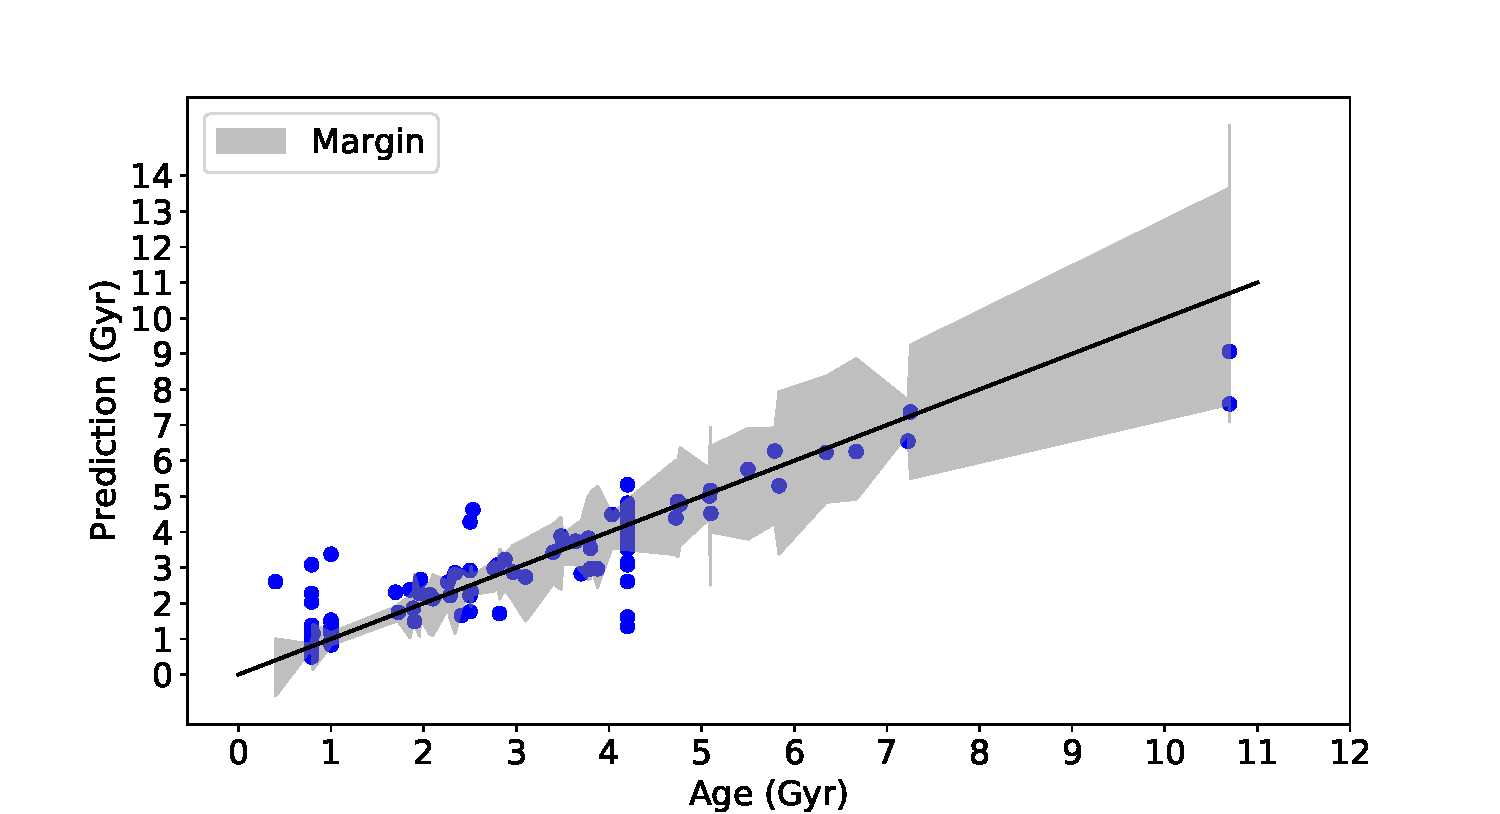
\includegraphics[width=0.8\linewidth]{Figuras/Experimentos/B_A_gp_1.pdf}
\end{center}
\caption{Benchmark A: Rendimiento para el modelo Gaussian Process.}
 \label{fig:benchA_details_gp_1}
\end{figure}

\begin{figure}[H]
\begin{center}
 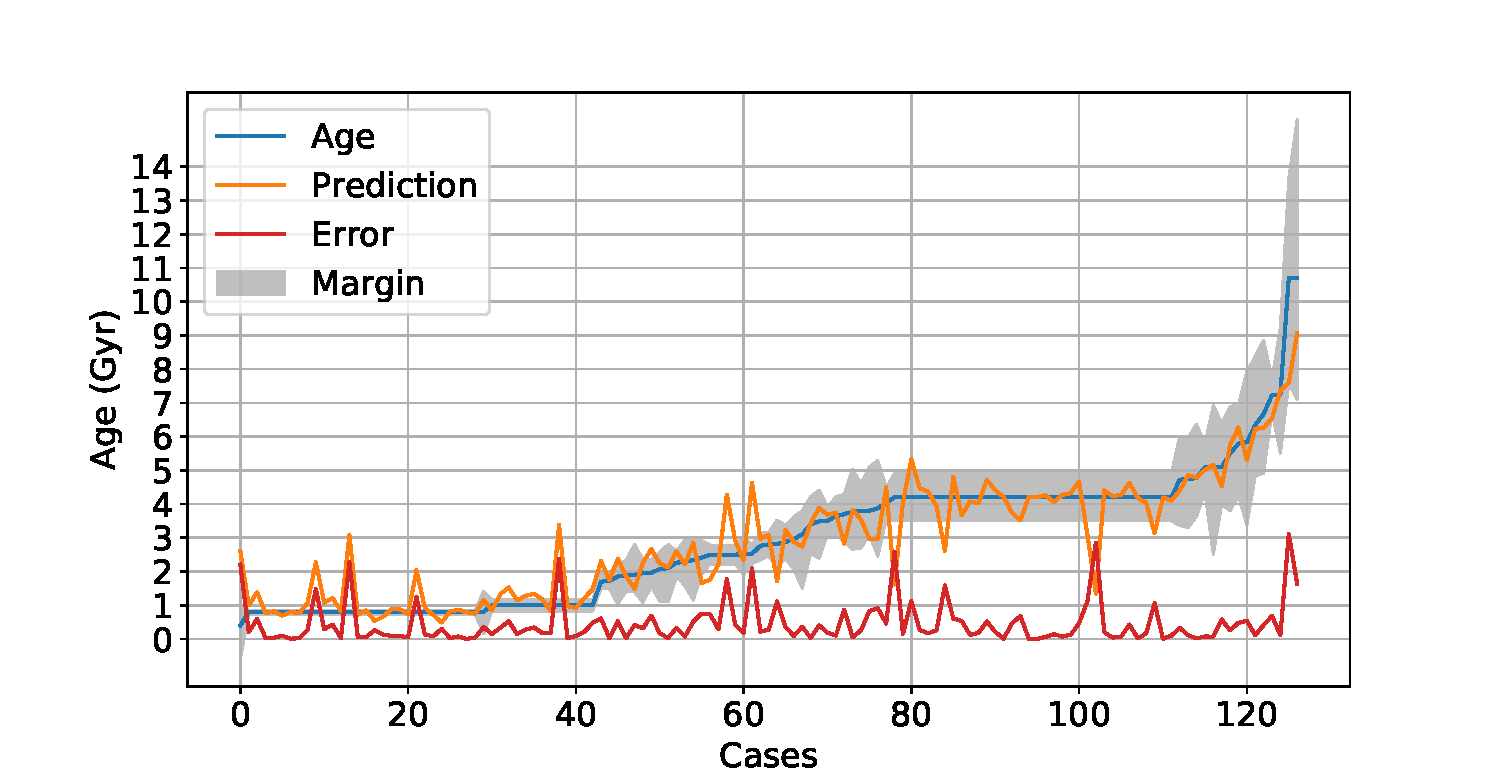
\includegraphics[width=0.8\linewidth]{Figuras/Experimentos/B_A_gp_2.pdf}
\end{center}
\caption{Benchmark A: Predicción detallada para el modelo de Gaussian Process. Se observa la edad real (en azul), la predicción de los modelos (en naranja), y el error correspondiente (en rojo).}
 \label{fig:benchA_details_gp_2}
\end{figure}

\begin{figure}[H]
\begin{center}
 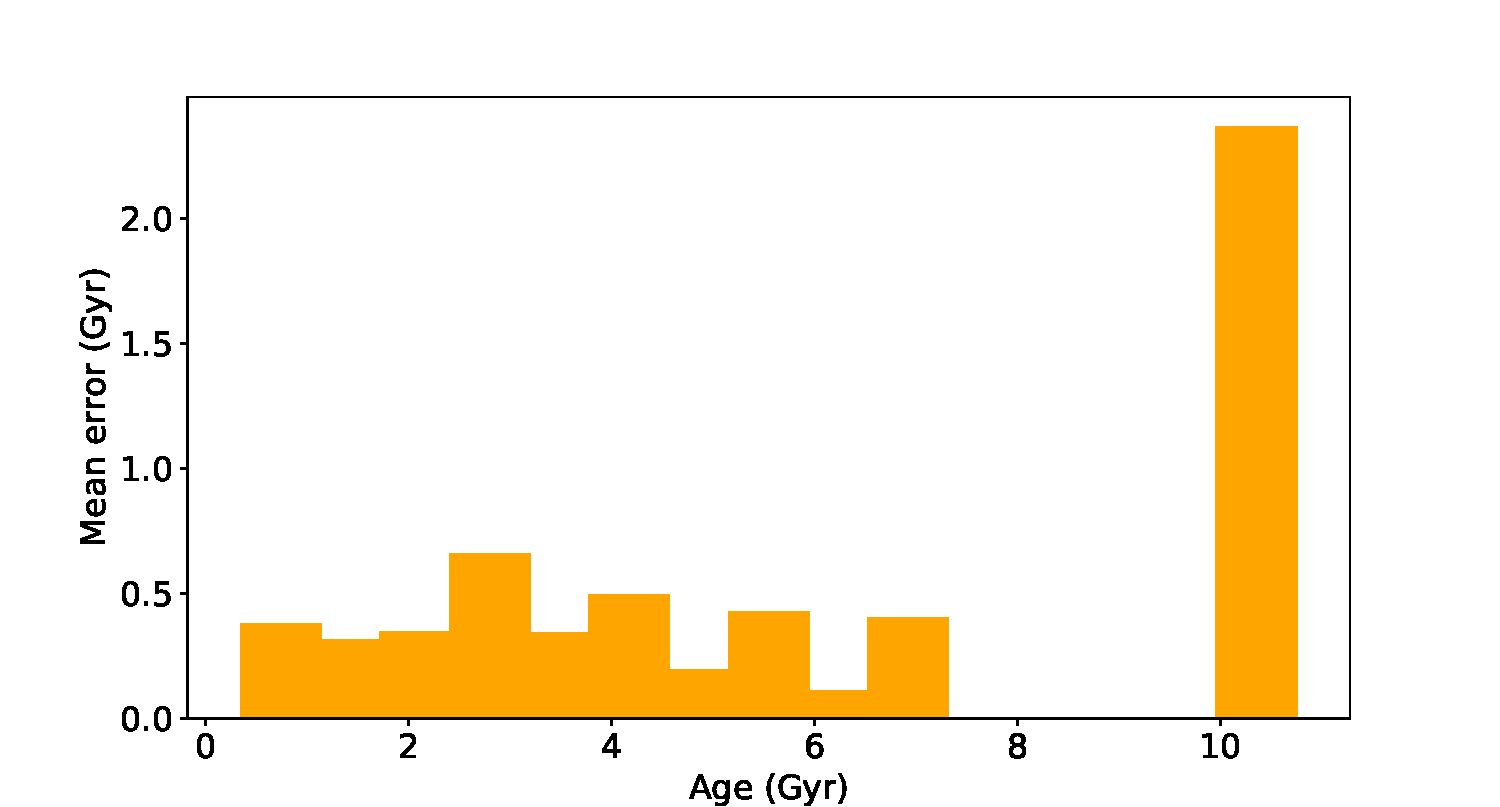
\includegraphics[width=0.8\linewidth]{Figuras/Experimentos/B_A_gp_3.pdf}
\end{center}
\caption{Benchmark A: MAE en función del rango de edad del conjunto de prueba.}
 \label{fig:benchA_details_gp_3}
\end{figure}

\paragraph{kNN} 
A continuación, se muestran las 3 gráficas que detallan el rendimiento del modelo kNN. El cual ha presentado una MAE de 0.532 Gyr.

\begin{figure}[H]
\begin{center}
 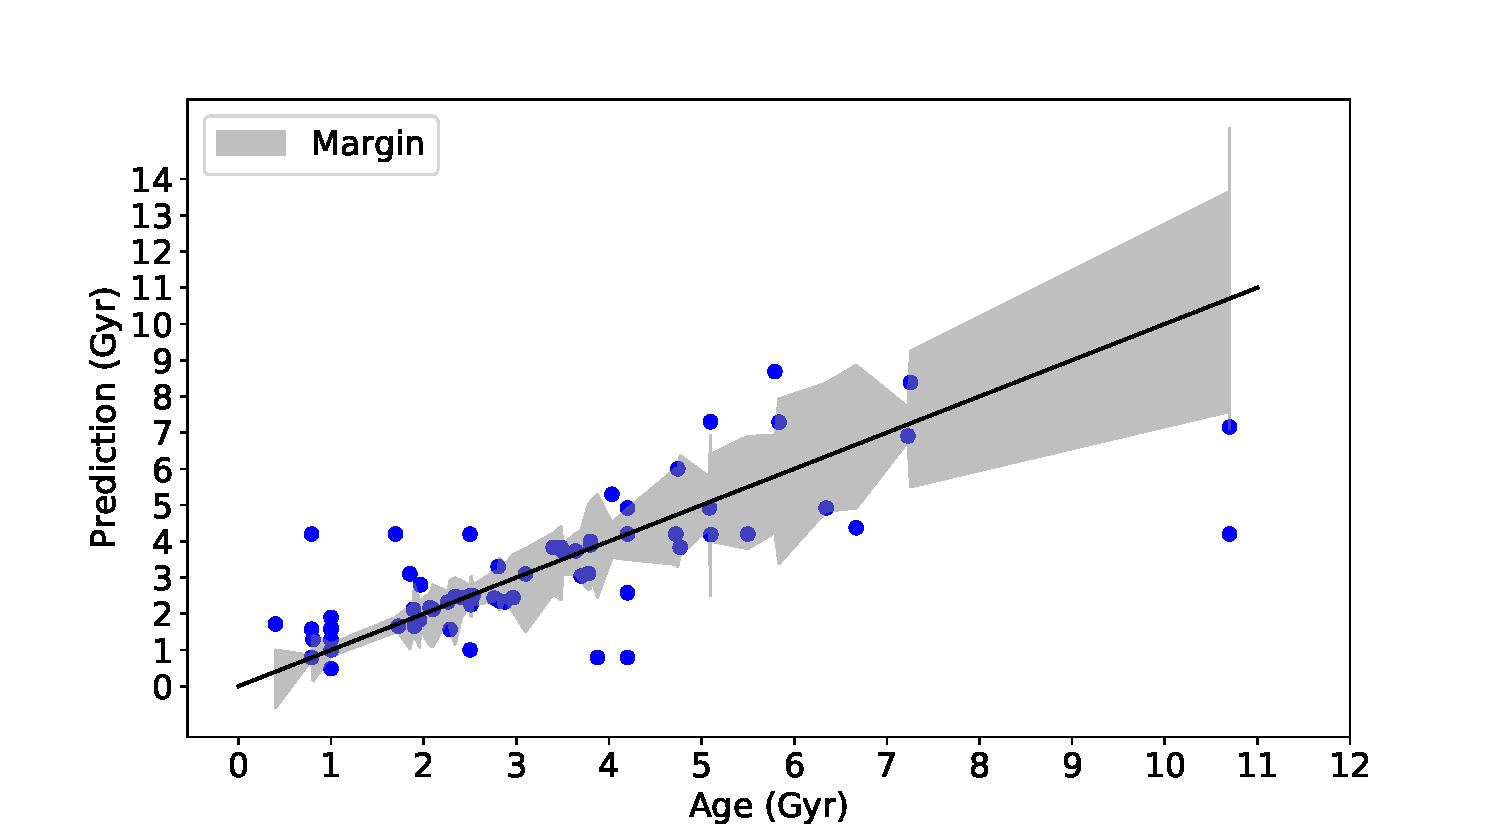
\includegraphics[width=0.8\linewidth]{Figuras/Experimentos/B_A_knn_1.pdf}
\end{center}
\caption{Benchmark A: Rendimiento para el modelo kNN.}
 \label{fig:benchA_details_knn_1}
\end{figure}

\begin{figure}[H]
\begin{center}
 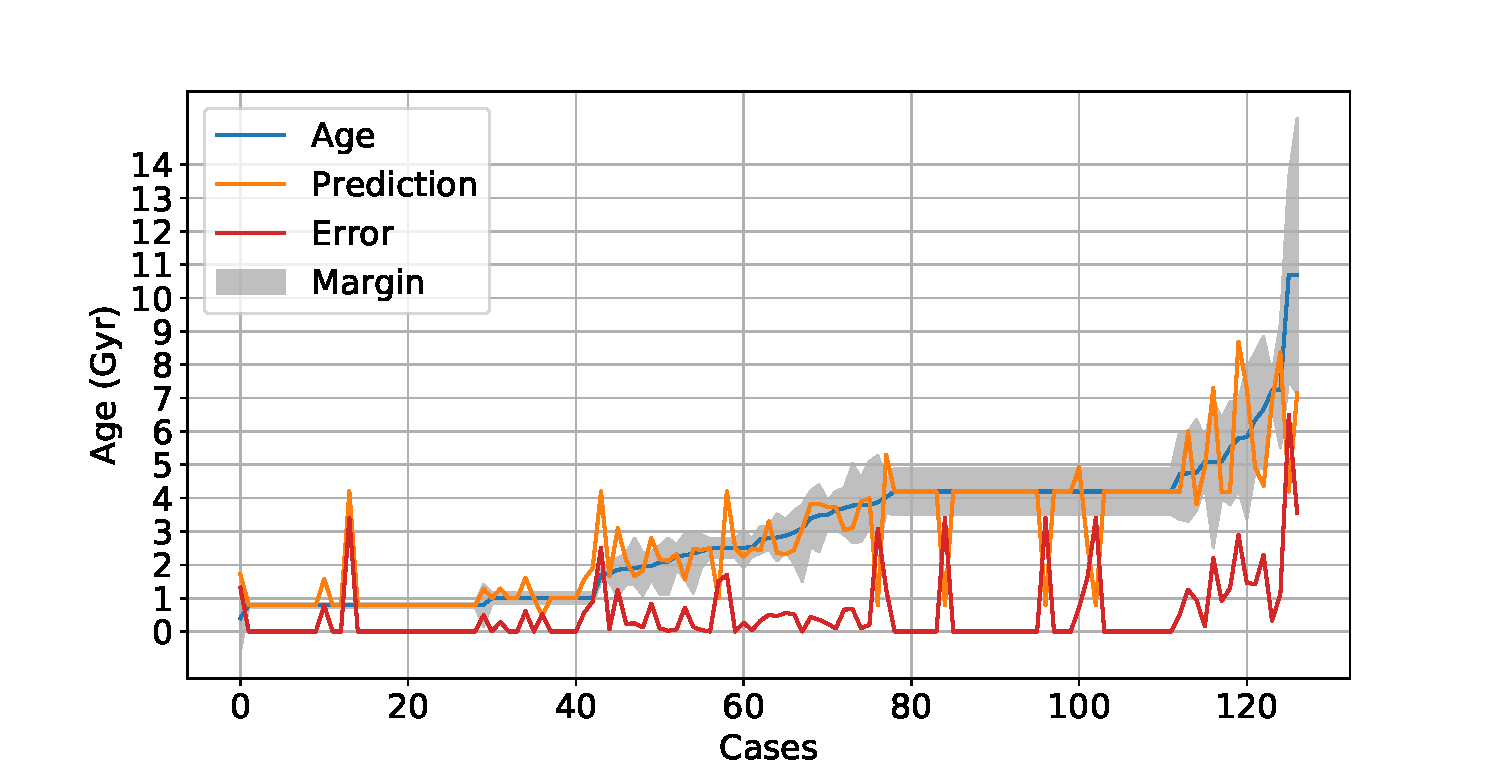
\includegraphics[width=0.8\linewidth]{Figuras/Experimentos/B_A_knn_2.pdf}
\end{center}
\caption{Benchmark A: Predicción detallada para el modelo de kNN. Se observa la edad real (en azul), la predicción de los modelos (en naranja), y el error correspondiente (en rojo).}
 \label{fig:benchA_details_knn_2}
\end{figure}

\begin{figure}[H]
\begin{center}
 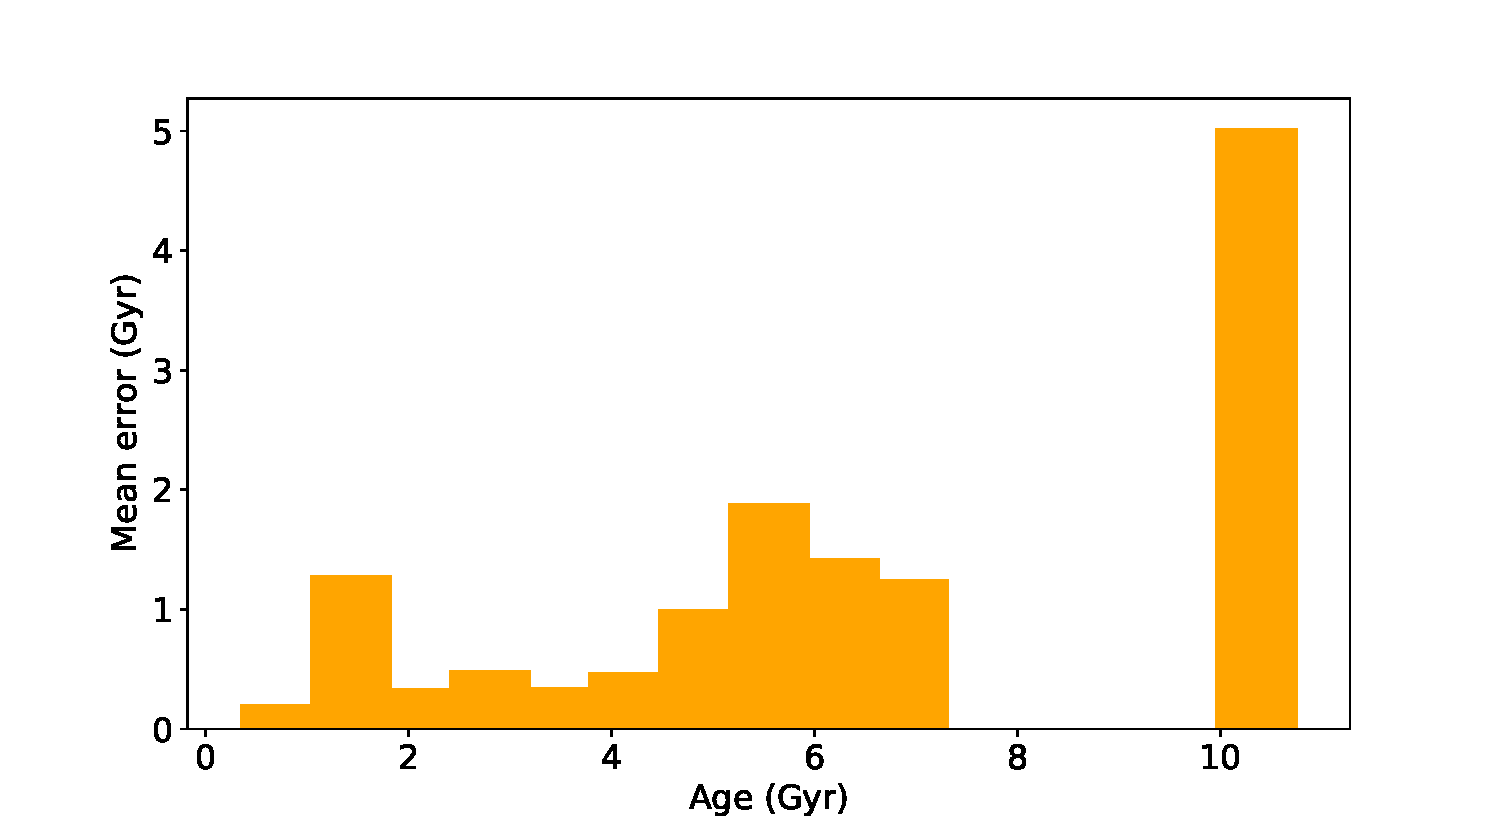
\includegraphics[width=0.8\linewidth]{Figuras/Experimentos/B_A_knn_3.pdf}
\end{center}
\caption{Benchmark A: MAE en función del rango de edad del conjunto de prueba.}
 \label{fig:benchA_details_knn_3}
\end{figure}

\paragraph{Random Forest} 
A continuación, se muestran las 3 gráficas que detallan el rendimiento del modelo Random Forest. El cual ha presentado una MAE de 0.572 Gyr.

\begin{figure}[H]
\begin{center}
 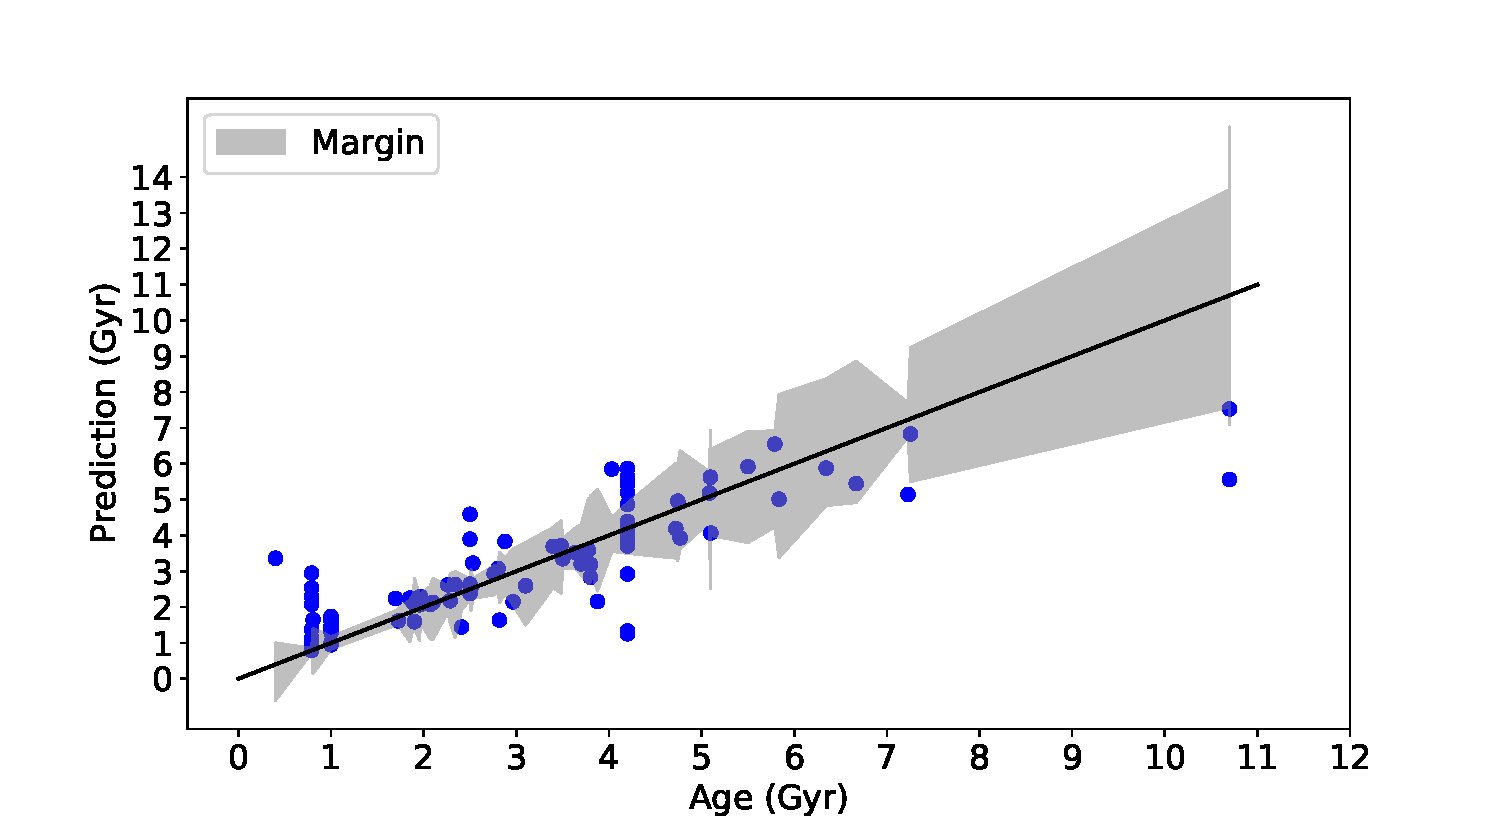
\includegraphics[width=0.8\linewidth]{Figuras/Experimentos/B_A_rf_1.pdf}
\end{center}
\caption{Benchmark A: Rendimiento para el modelo Random Forest.}
 \label{fig:benchA_details_rf_1}
\end{figure}

\begin{figure}[H]
\begin{center}
 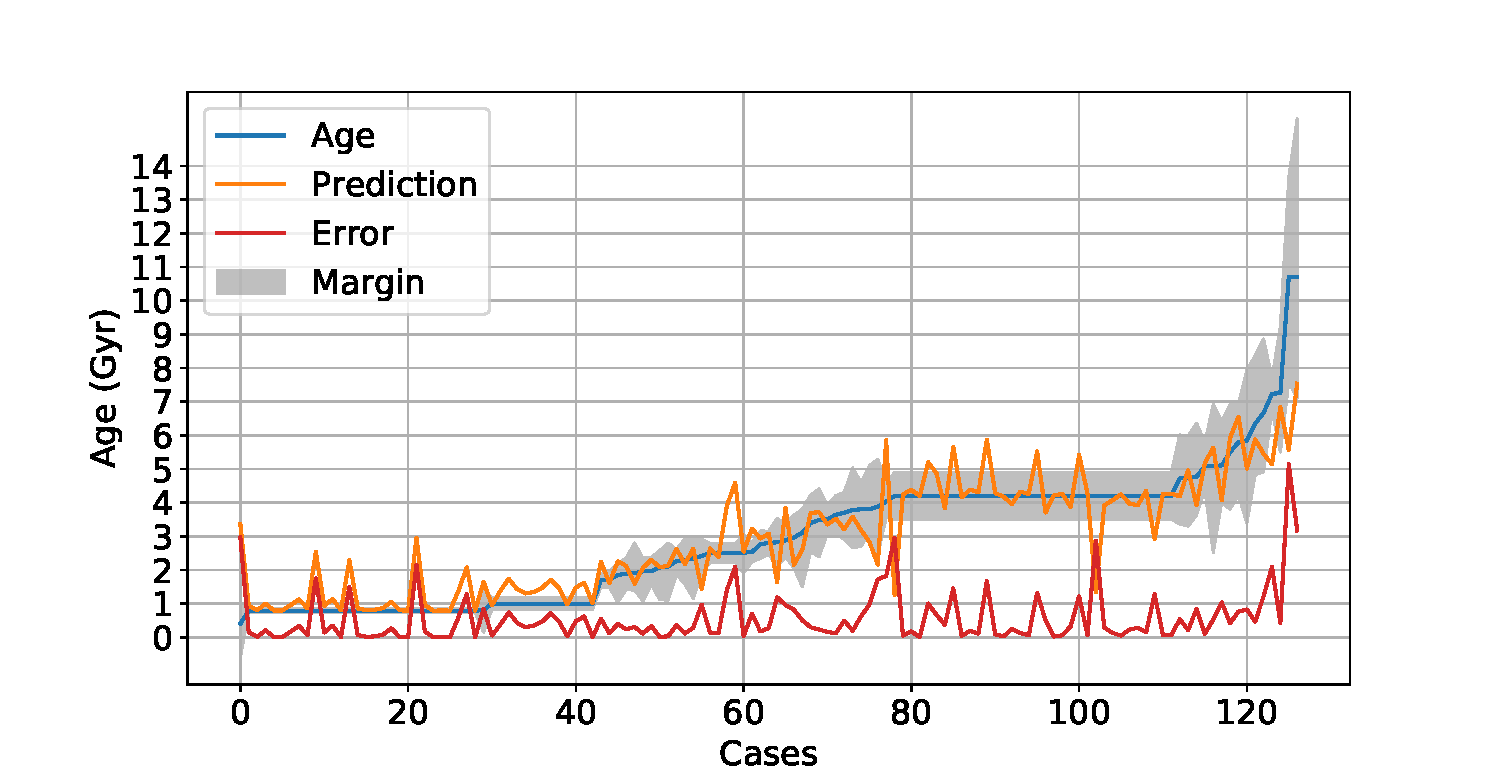
\includegraphics[width=0.8\linewidth]{Figuras/Experimentos/B_A_rf_2.pdf}
\end{center}
\caption{Benchmark A: Predicción detallada para el modelo de Random Forest. Se observa la edad real (en azul), la predicción de los modelos (en naranja), y el error correspondiente (en rojo).}
 \label{fig:benchA_details_rf_2}
\end{figure}

\begin{figure}[H]
\begin{center}
 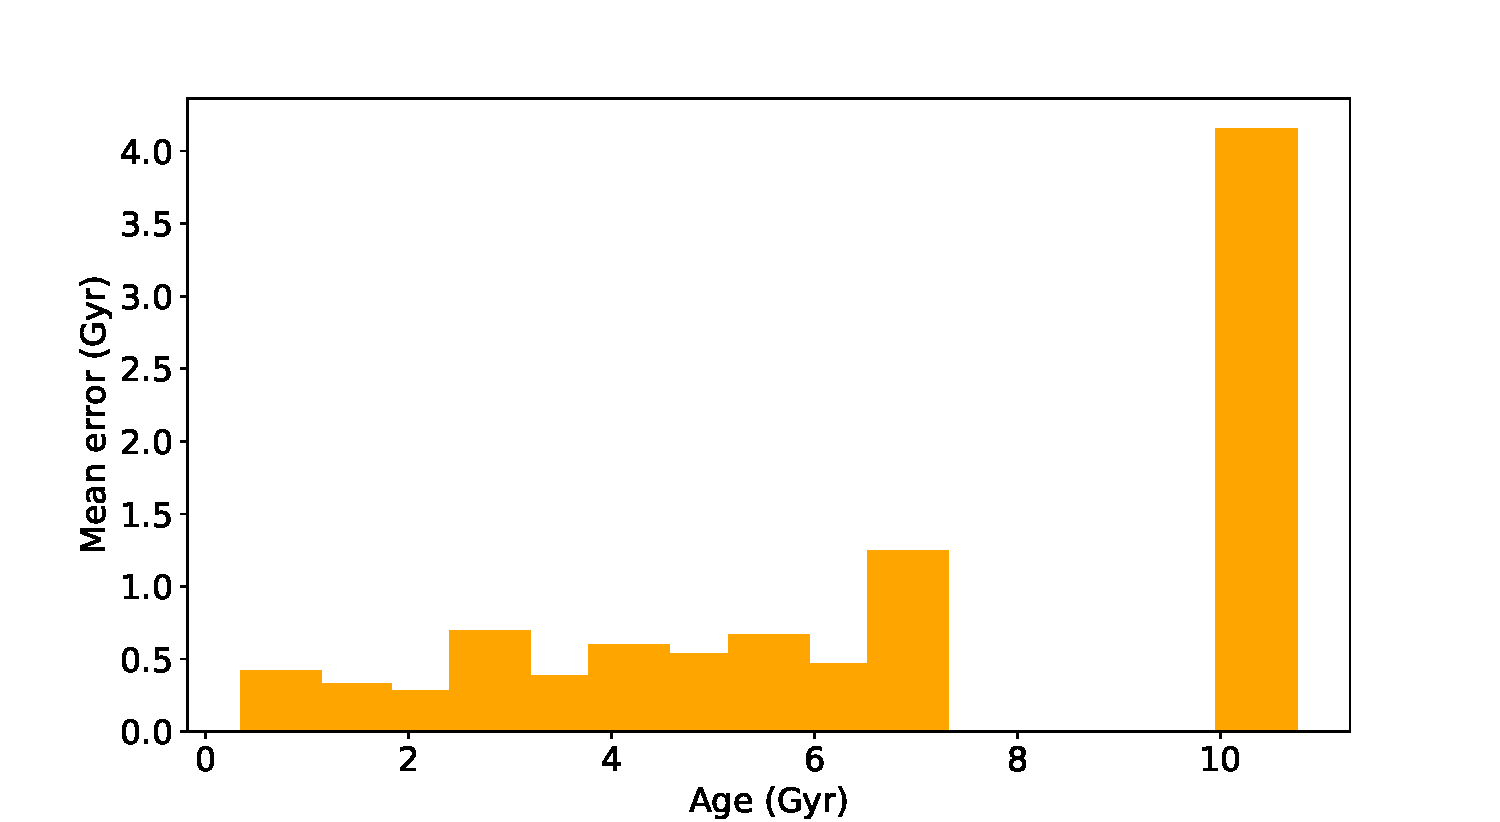
\includegraphics[width=0.8\linewidth]{Figuras/Experimentos/B_A_rf_3.pdf}
\end{center}
\caption{Benchmark A: MAE en función del rango de edad del conjunto de prueba.}
 \label{fig:benchA_details_rf_3}
\end{figure}

\paragraph{Support Vector Regression} 
A continuación, se muestran las 3 gráficas que detallan el rendimiento del modelo Support Vector Regression. El cual ha presentado una MAE de 0.676 Gyr.

\begin{figure}[H]
\begin{center}
 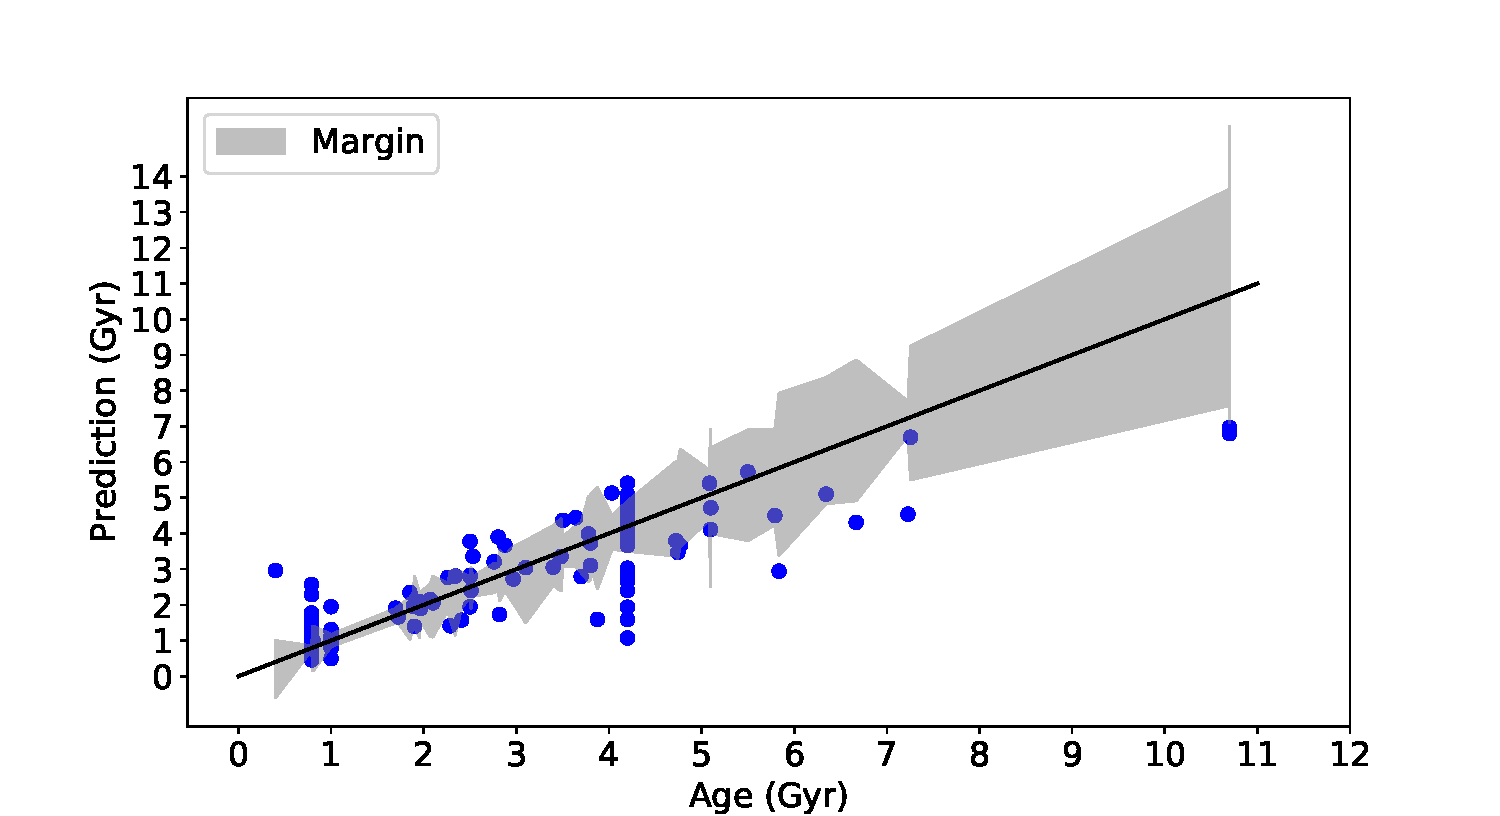
\includegraphics[width=0.8\linewidth]{Figuras/Experimentos/B_A_svm_1.pdf}
\end{center}
\caption{Benchmark A: Rendimiento para el modelo Support Vector Regression.}
 \label{fig:benchA_details_svm_1}
\end{figure}

\begin{figure}[H]
\begin{center}
 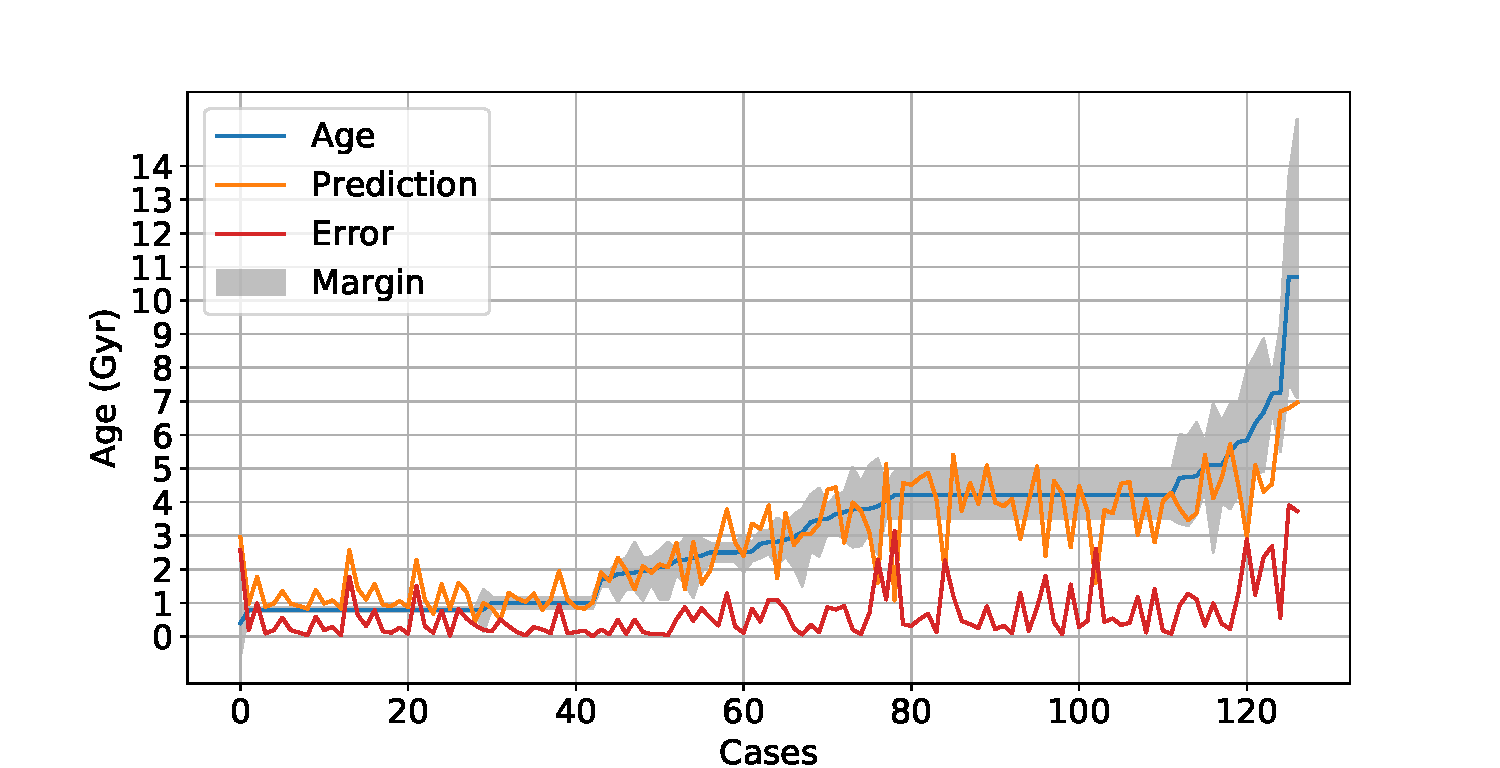
\includegraphics[width=0.8\linewidth]{Figuras/Experimentos/B_A_svm_2.pdf}
\end{center}
\caption{Benchmark A: Predicción detallada para el modelo de Support Vector Regression. Se observa la edad real (en azul), la predicción de los modelos (en naranja), y el error correspondiente (en rojo).}
 \label{fig:benchA_details_svm_2}
\end{figure}

\begin{figure}[H]
\begin{center}
 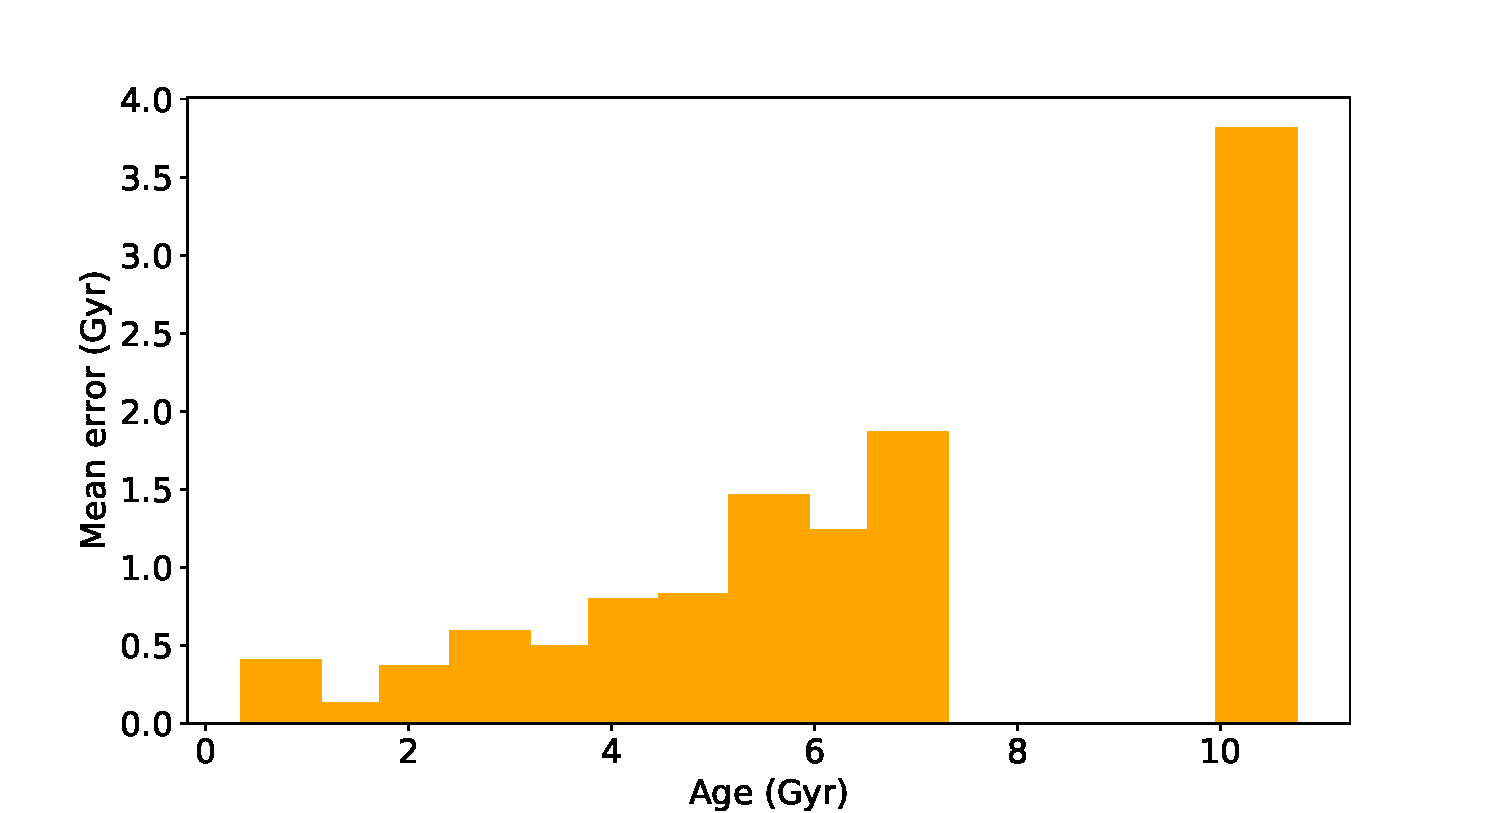
\includegraphics[width=0.8\linewidth]{Figuras/Experimentos/B_A_svm_3.pdf}
\end{center}
\caption{Benchmark A: MAE en función del rango de edad del conjunto de prueba.}
 \label{fig:benchA_details_svm_3}
\end{figure}

\paragraph{Decision Tree Regression} 
A continuación, se muestran las 3 gráficas que detallan el rendimiento del modelo Decision Tree Regression. El cual ha presentado una MAE de 0.695 Gyr.

\begin{figure}[H]
\begin{center}
 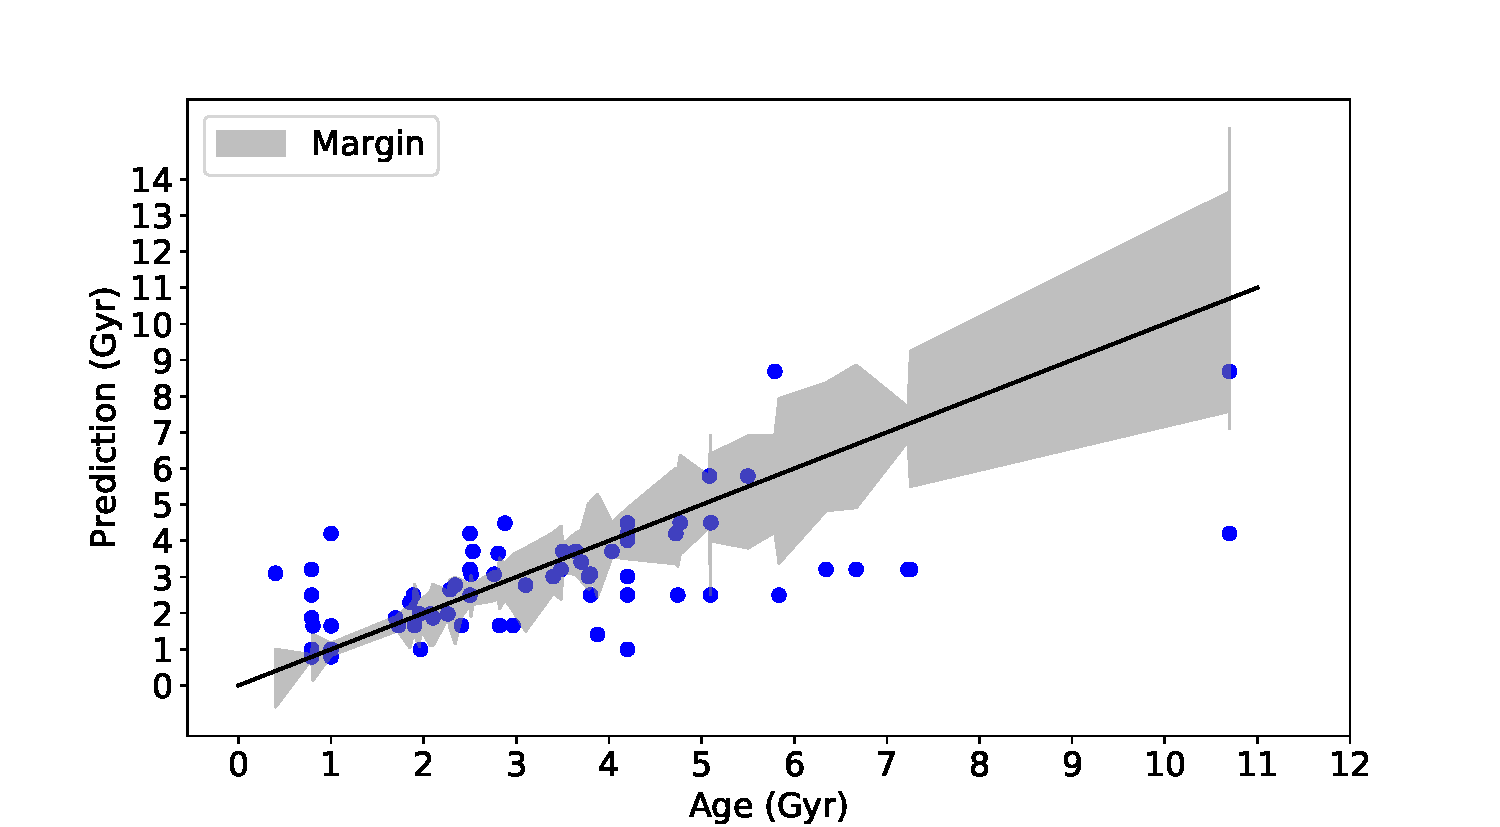
\includegraphics[width=0.8\linewidth]{Figuras/Experimentos/B_A_dtr_1.pdf}
\end{center}
\caption{Benchmark A: Rendimiento para el modelo Decision Tree Regression.}
 \label{fig:benchA_details_dtr_1}
\end{figure}

\begin{figure}[H]
\begin{center}
 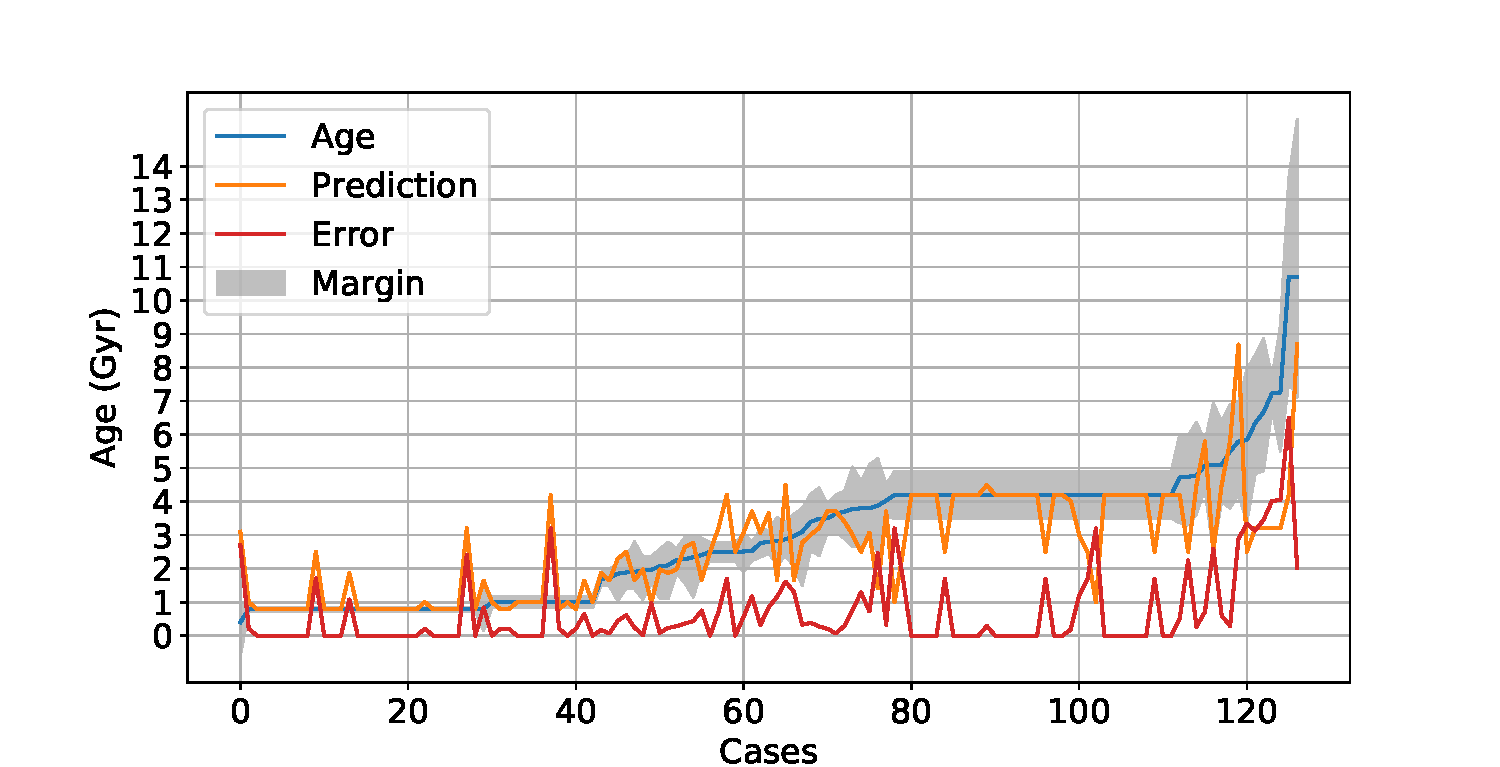
\includegraphics[width=0.8\linewidth]{Figuras/Experimentos/B_A_dtr_2.pdf}
\end{center}
\caption{Benchmark A: Predicción detallada para el modelo de Decision Tree Regression. Se observa la edad real (en azul), la predicción de los modelos (en naranja), y el error correspondiente (en rojo).}
 \label{fig:benchA_details_dtr_2}
\end{figure}

\begin{figure}[H]
\begin{center}
 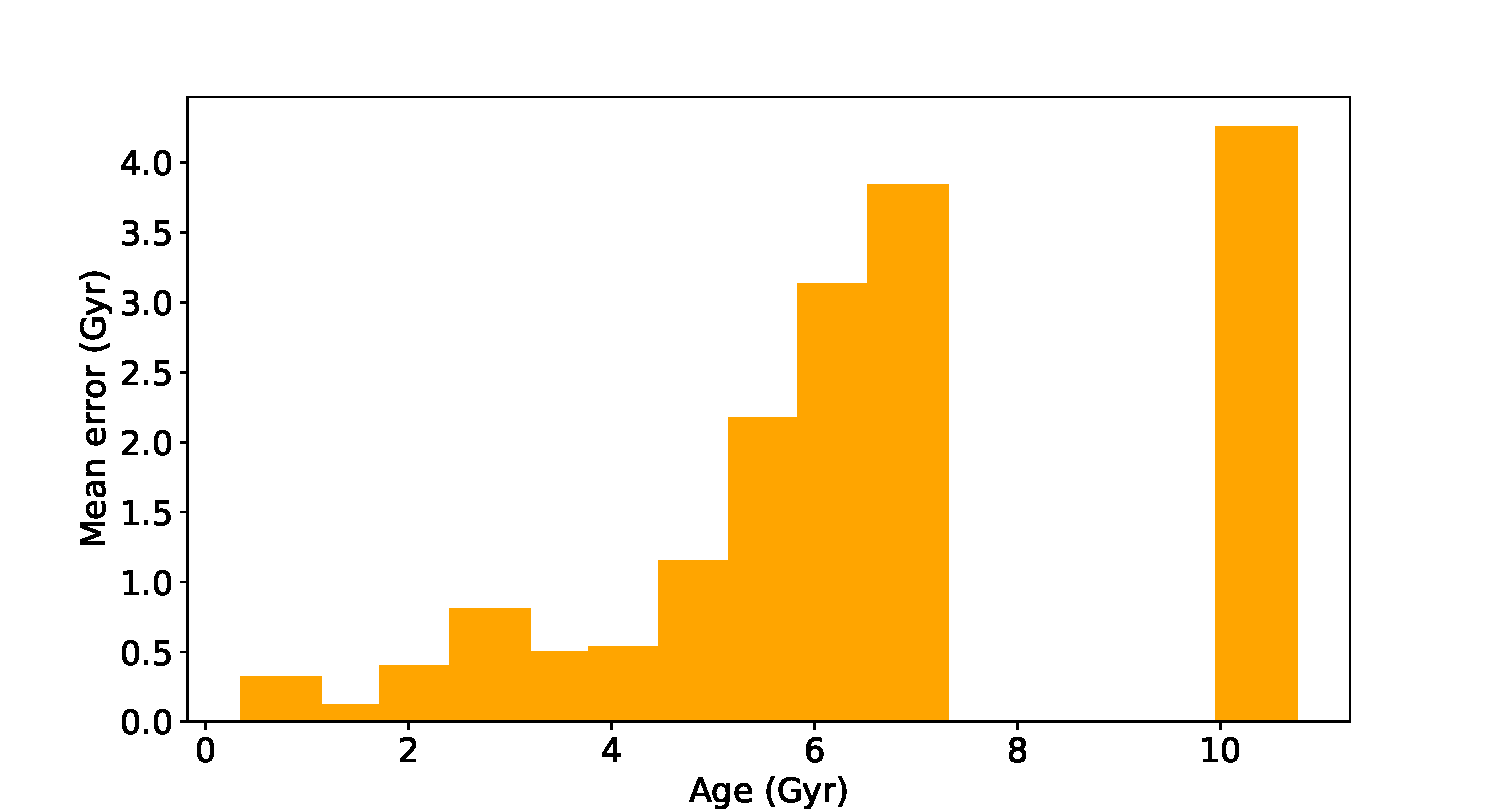
\includegraphics[width=0.8\linewidth]{Figuras/Experimentos/B_A_dtr_3.pdf}
\end{center}
\caption{Benchmark A: MAE en función del rango de edad del conjunto de prueba.}
 \label{fig:benchA_details_dtr_3}
\end{figure}

\paragraph{Linear Regressor} 
A continuación, se muestran las 3 gráficas que detallan el rendimiento del modelo Linear Regressor. El peor modelo de este benchmark junto con Bayesian Regression con un MAE de 0.951 Gyr.

\begin{figure}[H]
\begin{center}
 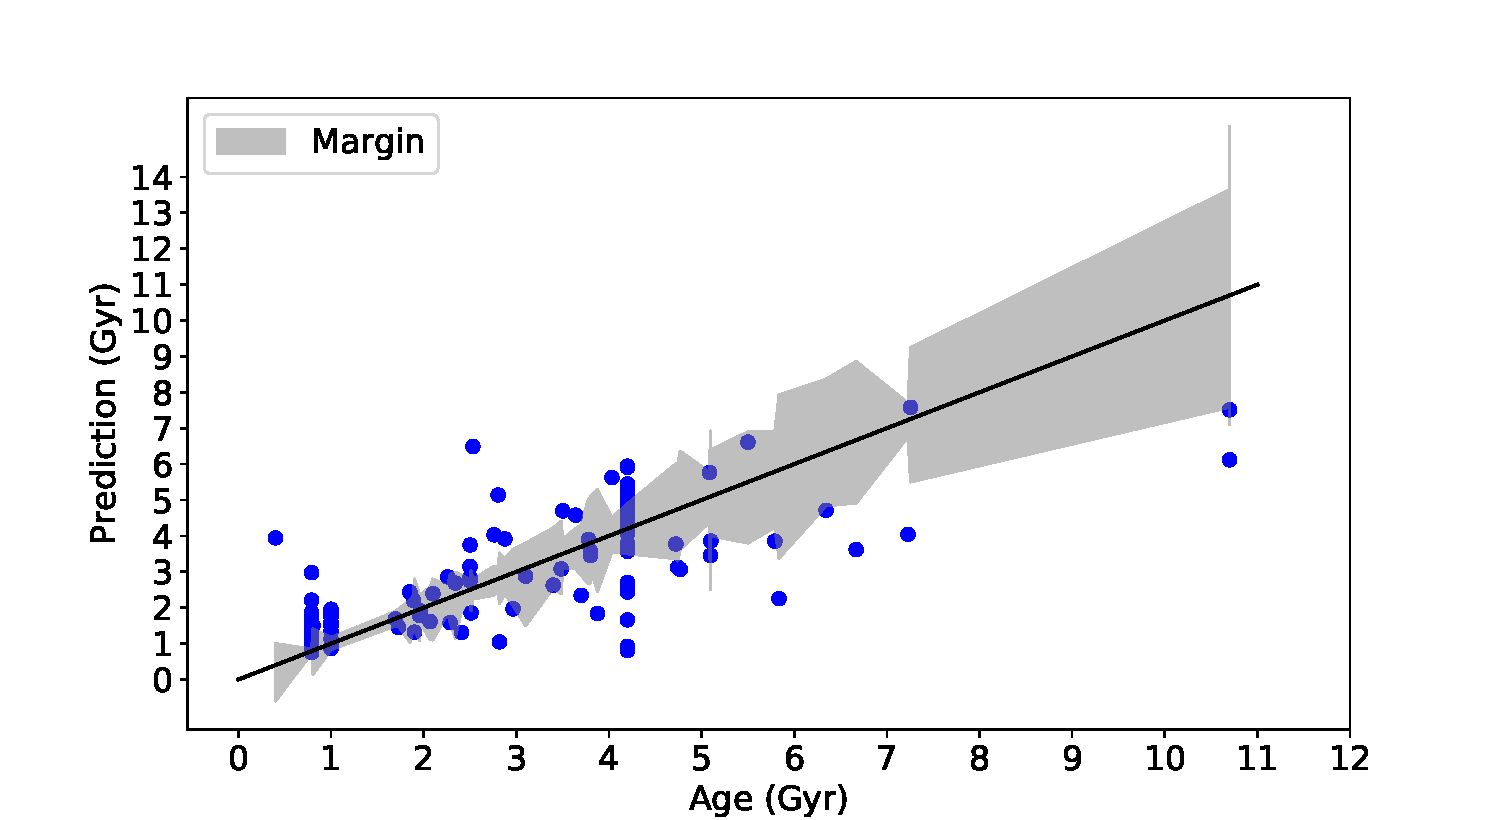
\includegraphics[width=0.8\linewidth]{Figuras/Experimentos/B_A_lr_1.pdf}
\end{center}
\caption{Benchmark A: Rendimiento para el modelo Linear Regressor.}
 \label{fig:benchA_details_lr_1}
\end{figure}

\begin{figure}[H]
\begin{center}
 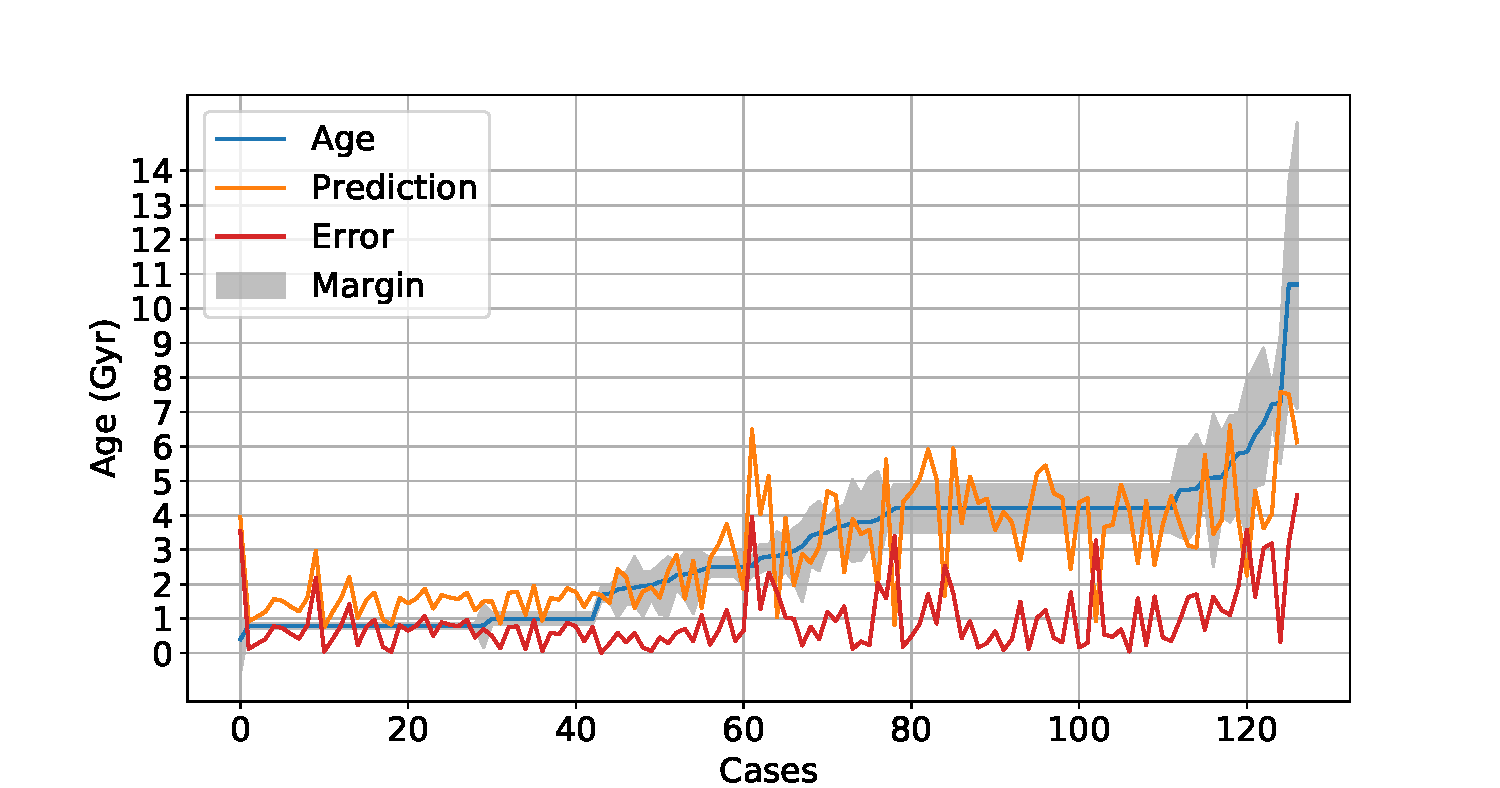
\includegraphics[width=0.8\linewidth]{Figuras/Experimentos/B_A_lr_2.pdf}
\end{center}
\caption{Benchmark A: Predicción detallada para el modelo de Linear Regressor. Se observa la edad real (en azul), la predicción de los modelos (en naranja), y el error correspondiente (en rojo).}
 \label{fig:benchA_details_lr_2}
\end{figure}

\begin{figure}[H]
\begin{center}
 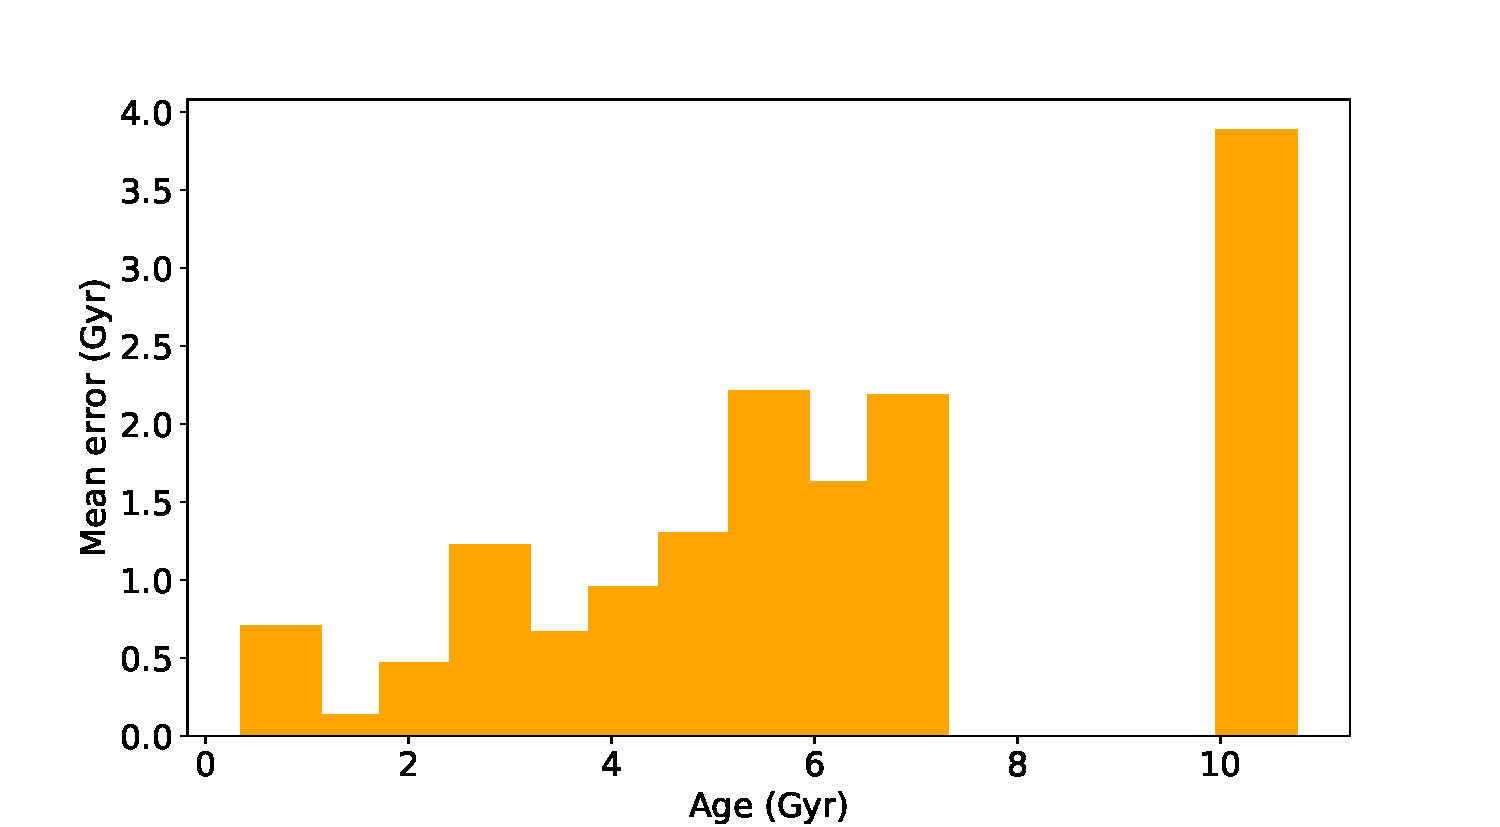
\includegraphics[width=0.8\linewidth]{Figuras/Experimentos/B_A_lr_3.pdf}
\end{center}
\caption{Benchmark A: MAE en función del rango de edad del conjunto de prueba.}
 \label{fig:benchA_details_lr_3}
\end{figure}

\paragraph{Bayesian Regression} 
A continuación, se muestran las 3 gráficas que detallan el rendimiento del modelo Bayesian Regression. El peor modelo de este benchmark junto con Linear Regressor con un MAE de 0.951 Gyr.

\begin{figure}[H]
\begin{center}
 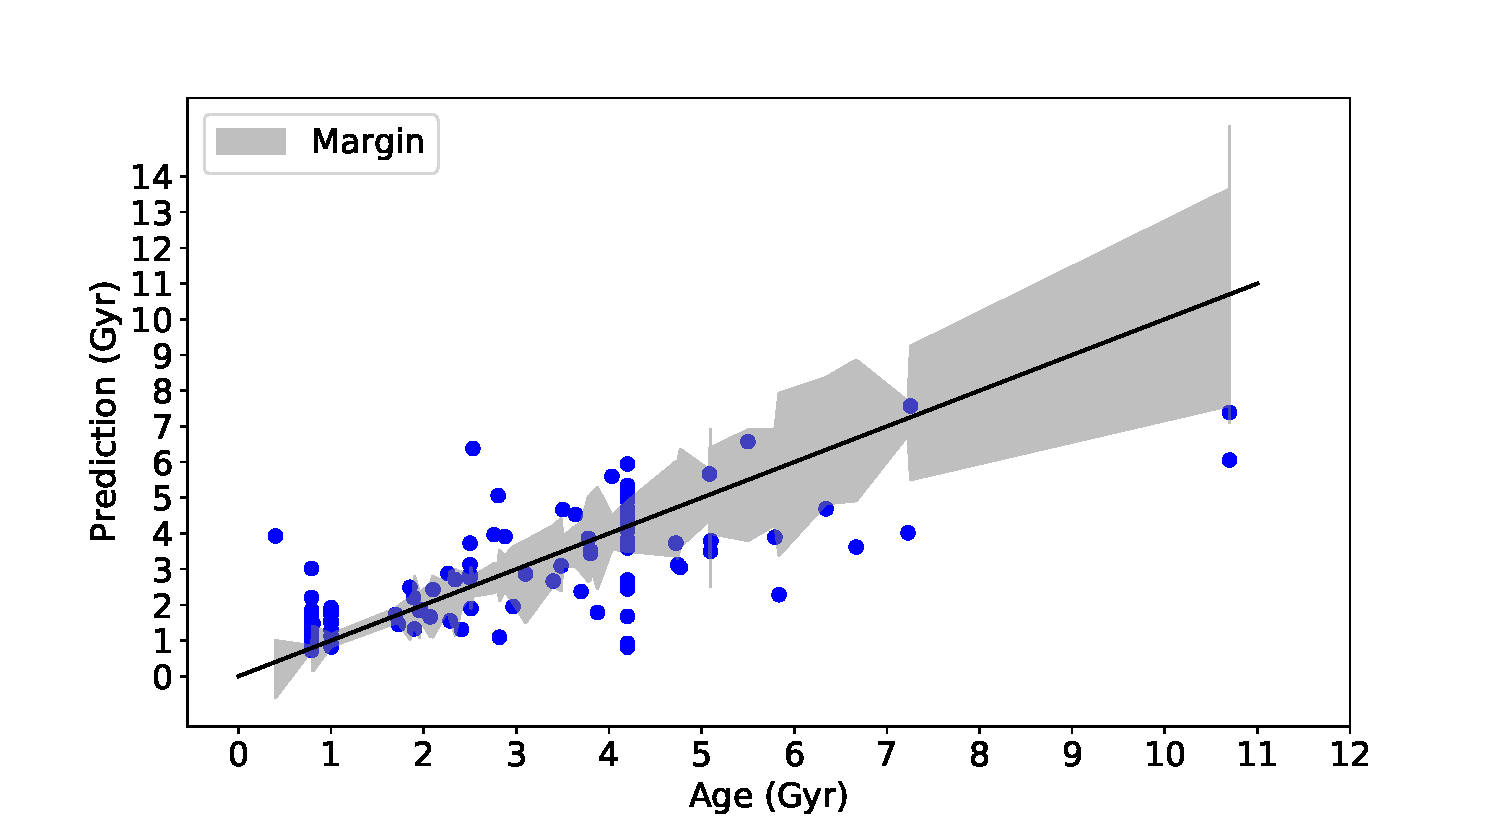
\includegraphics[width=0.8\linewidth]{Figuras/Experimentos/B_A_bayes_1.pdf}
\end{center}
\caption{Benchmark A: Rendimiento para el modelo Bayesian Regression.}
 \label{fig:benchA_details_bayes_1}
\end{figure}

\begin{figure}[H]
\begin{center}
 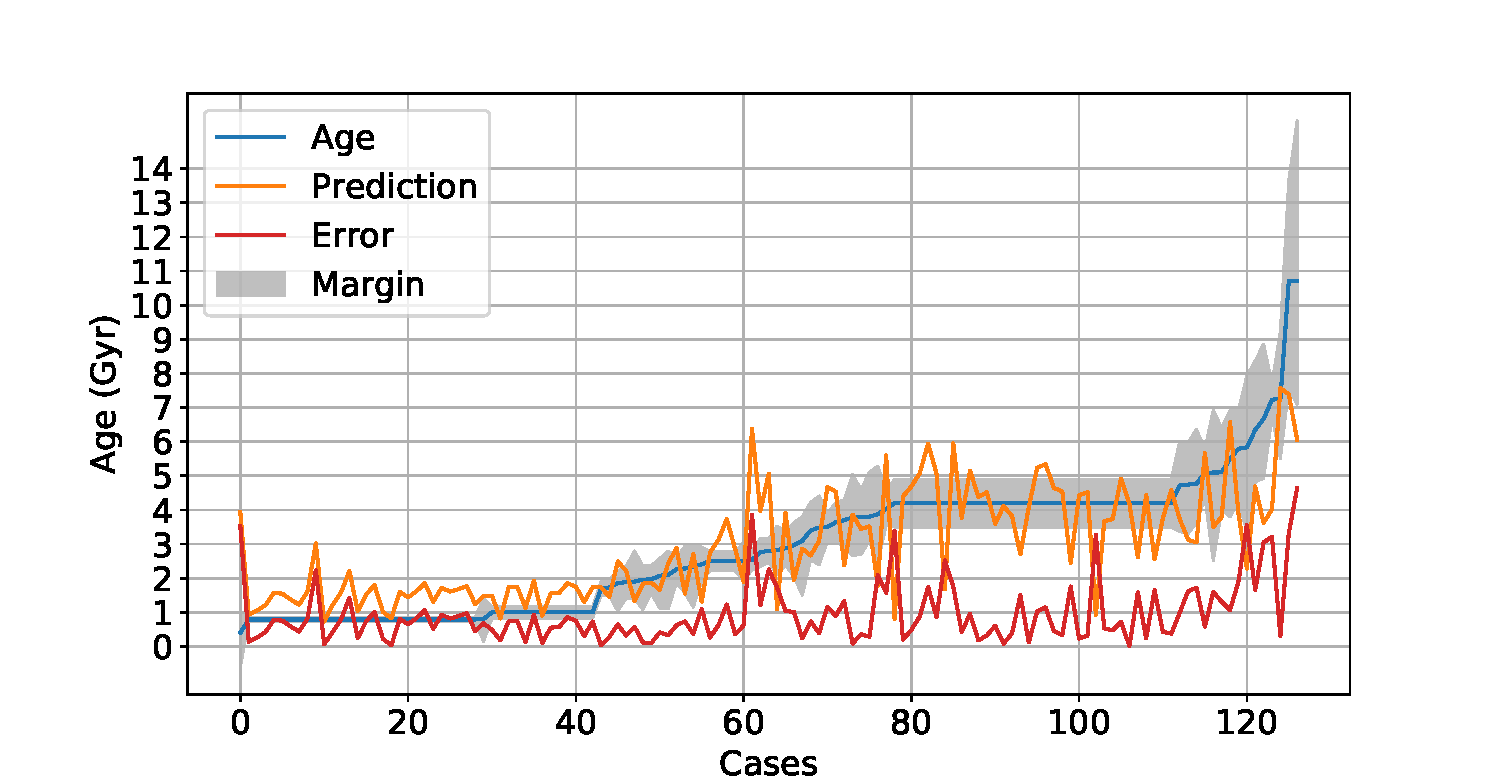
\includegraphics[width=0.8\linewidth]{Figuras/Experimentos/B_A_bayes_2.pdf}
\end{center}
\caption{Benchmark A: Predicción detallada para el modelo de Bayesian Regression. Se observa la edad real (en azul), la predicción de los modelos (en naranja), y el error correspondiente (en rojo).}
 \label{fig:benchA_details_bayes_2}
\end{figure}

\begin{figure}[H]
\begin{center}
 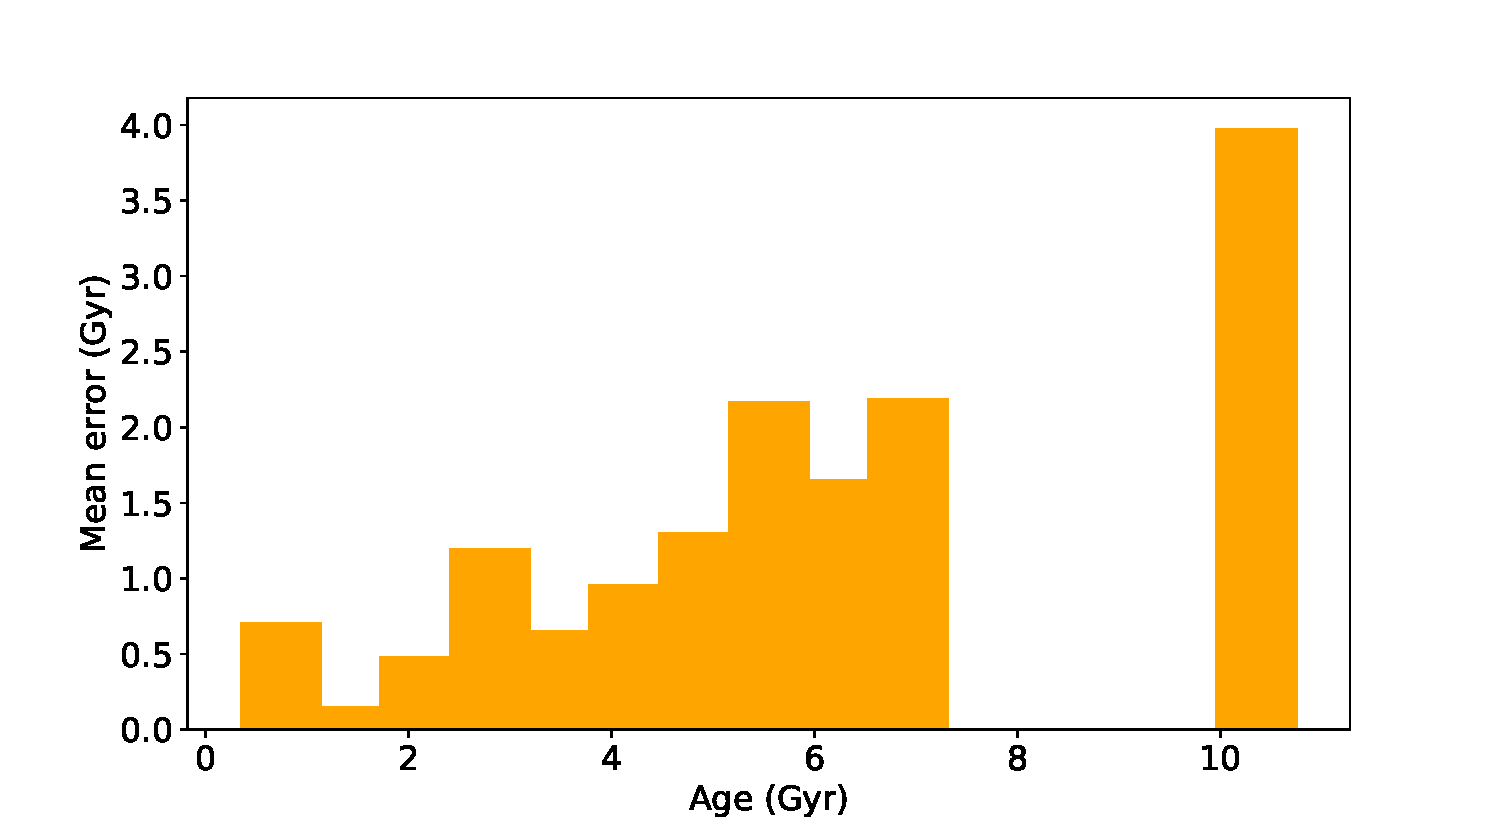
\includegraphics[width=0.8\linewidth]{Figuras/Experimentos/B_A_bayes_3.pdf}
\end{center}
\caption{Benchmark A: MAE en función del rango de edad del conjunto de prueba.}
 \label{fig:benchA_details_bayes_3}
\end{figure}


\subsection{Benchmark B: Escenario de generalización}

Aquí se analiza la capacidad de generalización de todos los modelos para el problema de datación estelar. Las Figuras \ref{fig:benchB1} y \ref{fig:benchB2} muestran el rendimiento en los escenarios de evaluación B1 y B2, respectivamente.

\begin{figure}[H]
\begin{center}
 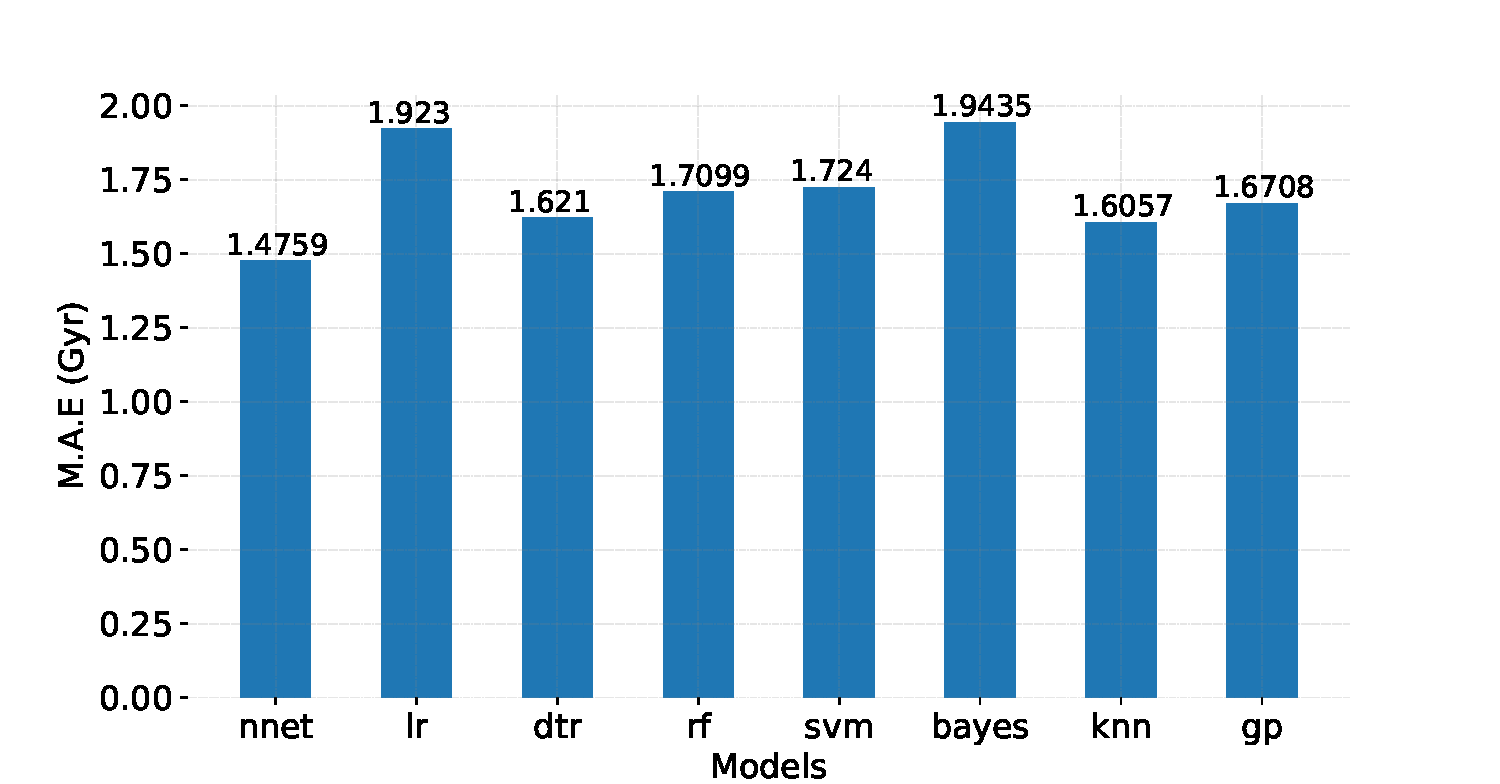
\includegraphics[width=0.8\linewidth]{Figuras/Experimentos/B_B1_models.pdf}
\end{center}
\caption{Benchmark B1: Rendimiento de los modelos en función del MAE.}
 \label{fig:benchB1}
\end{figure}

\begin{figure}[H]
\begin{center}
 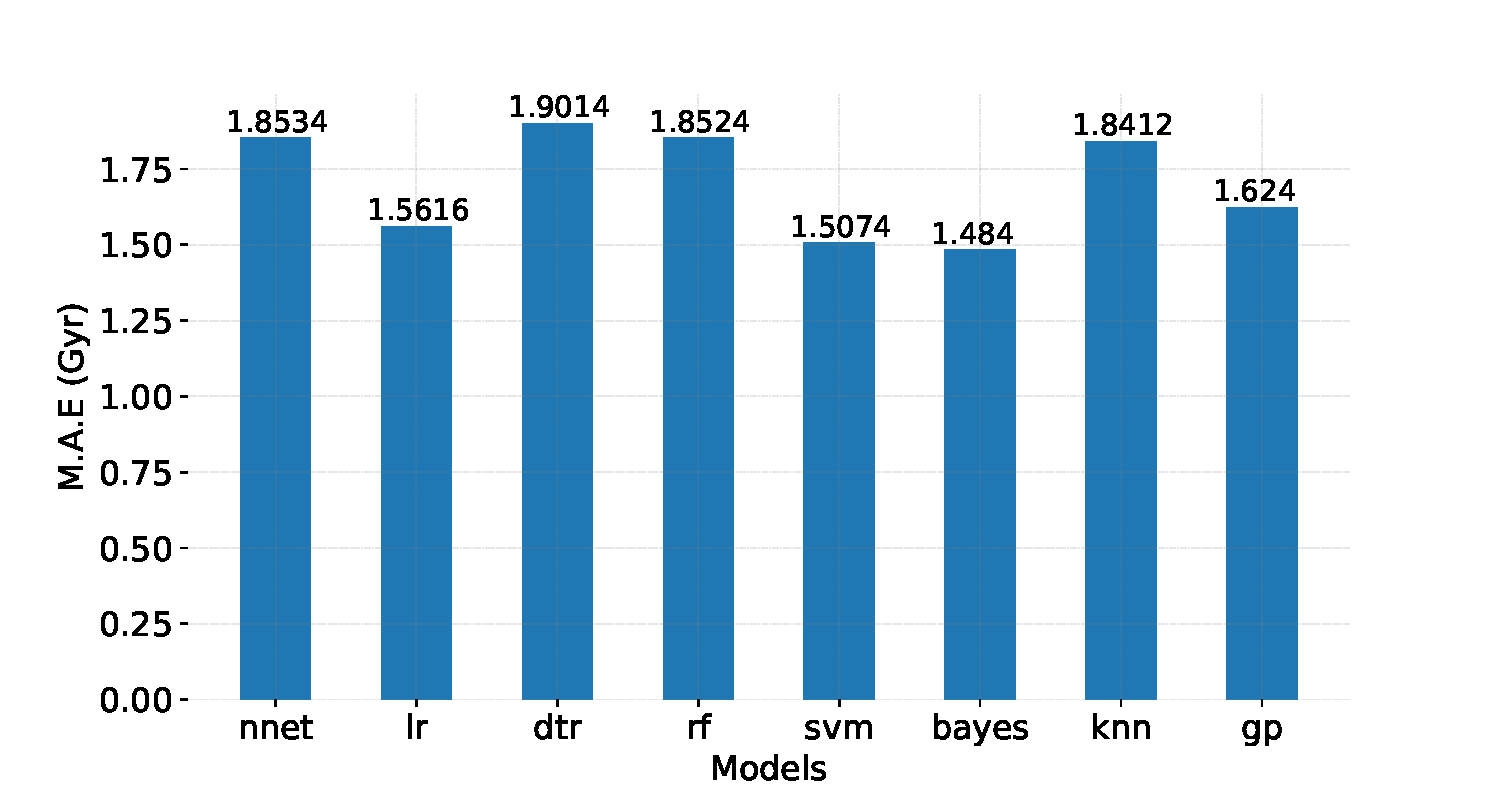
\includegraphics[width=0.8\linewidth]{Figuras/Experimentos/B_B2_models.pdf}
\end{center}
\caption{Benchmark B2: Rendimiento de los modelos en función del MAE.}
 \label{fig:benchB2}
\end{figure}

\subsubsection{Benchmark B1} 

El Benchmark B1 se centra en analizar la precisión de los modelos estimando edades de estrellas más antiguas a las que han visto durante el entrenamiento. Obviamente, el error promedio de lo modelos ha aumentado. El mejor rendimiento se observa en la Red Neuronal, con un MAE de 1,47 Gyr. Las estimaciones detalladas se pueden ver en la Figura \ref{fig:benchB1_best_1} y Figura \ref{fig:benchB1_best_2}, donde se puede observar cómo la Red Neuronal es capaz de generalizar hasta 6 Gyr, asignando estimaciones de edad que en su mayoría se encuentran dentro del margen de confianza. La Tabla \ref{table:precisions} confirma este hecho, donde la Red Neuronal también exhibe la precisión más alta para el Benchmark B1.

\paragraph{Neural Network} 
A continuación, se muestran las 3 gráficas que detallan el rendimiento del modelo Neural Network, el cual presenta el menor MAE de este benchmark, 1.475 Gyr.

\begin{figure}[H]
\begin{center}
 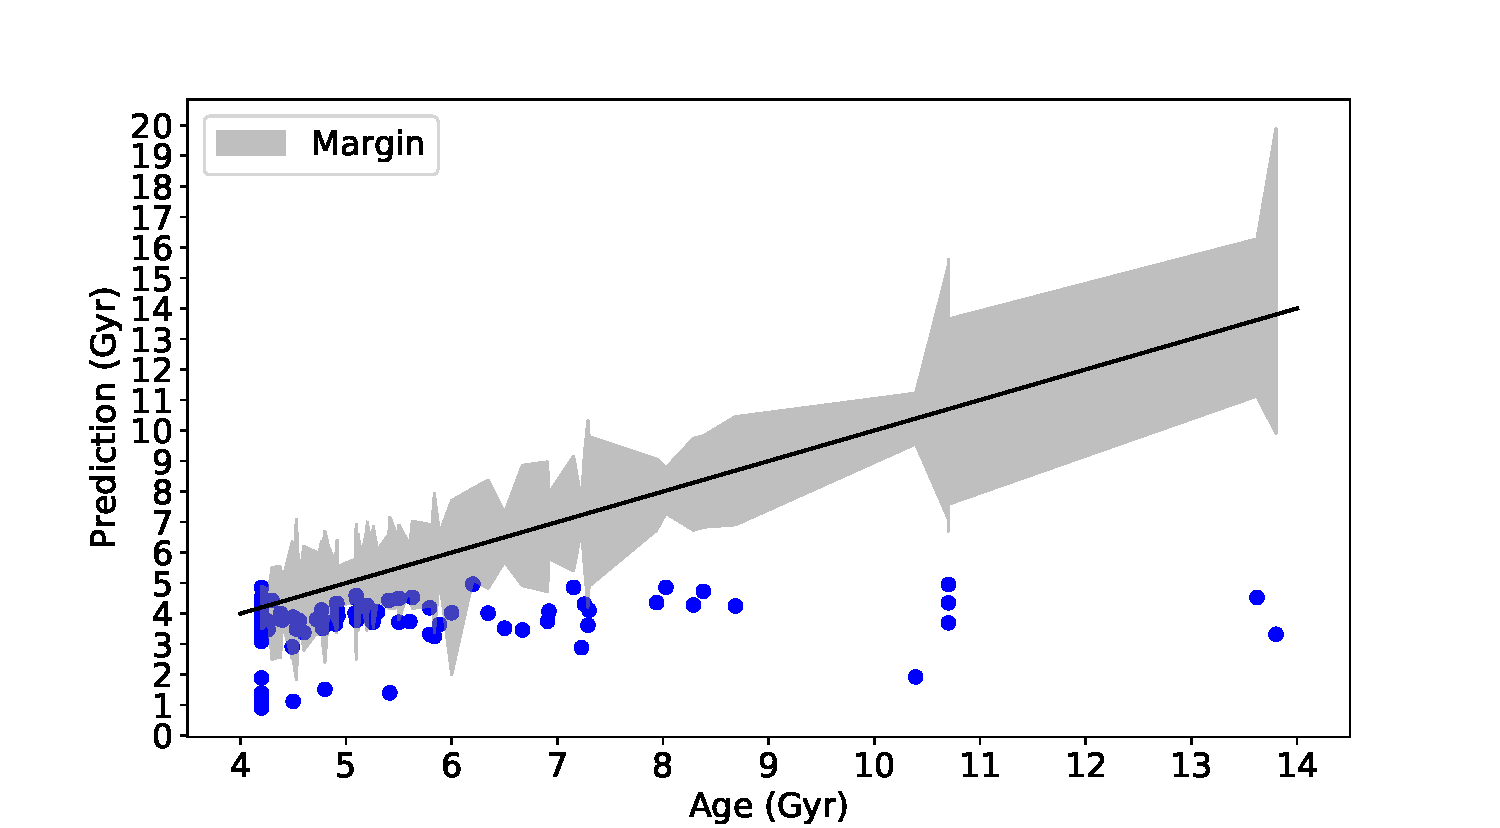
\includegraphics[width=0.8\linewidth]{Figuras/Experimentos/B_B1_nnet_1.pdf}
\end{center}
\caption{Benchmark B1: Rendimiento para el modelo Neural Network.}
 \label{fig:benchB1_best_1}
\end{figure}

\begin{figure}[H]
\begin{center}
 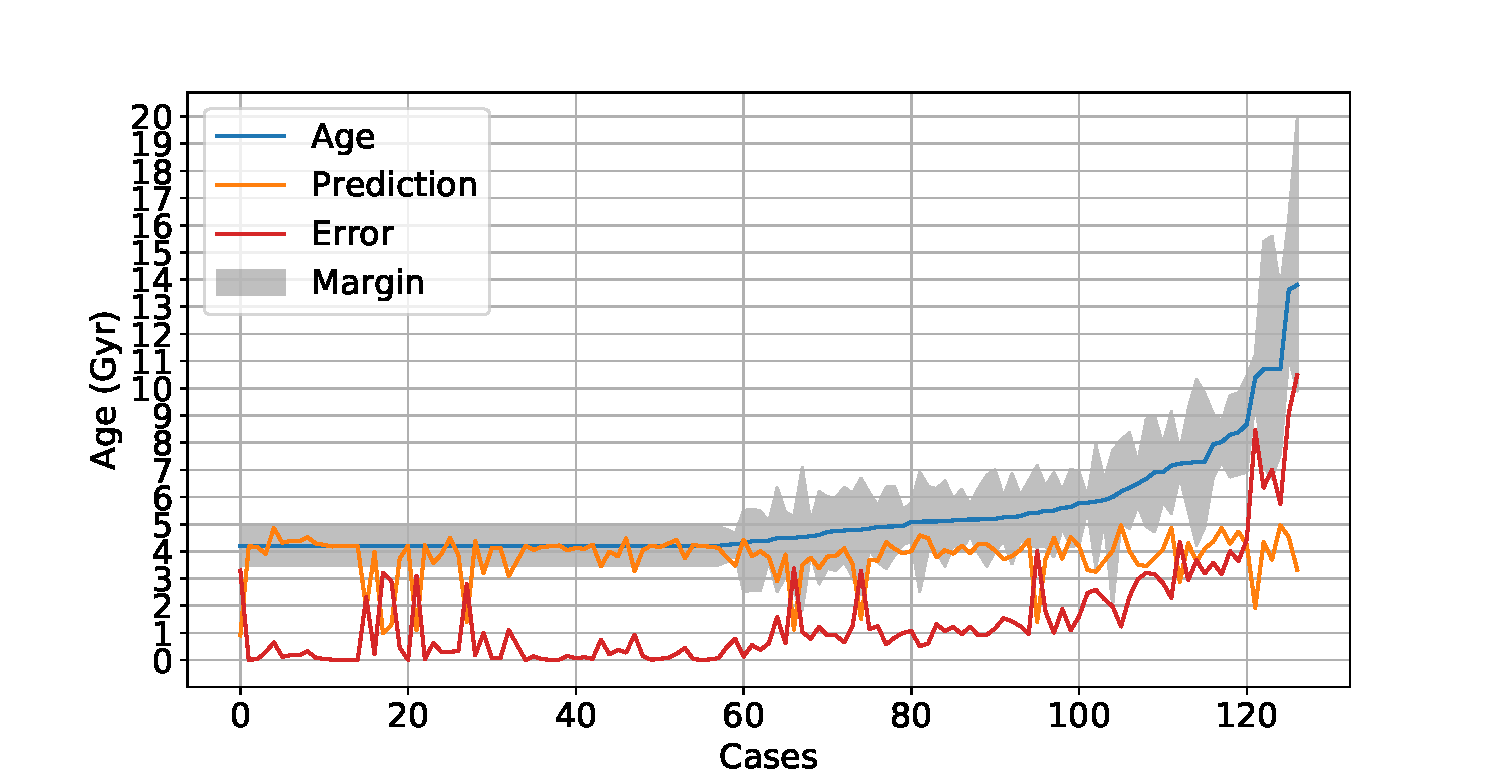
\includegraphics[width=0.8\linewidth]{Figuras/Experimentos/B_B1_nnet_2.pdf}
\end{center}
\caption{Benchmark B1: Predicción detallada para el modelo de Neural Network. Se observa la edad real (en azul), la predicción de los modelos (en naranja), y el error correspondiente (en rojo).}
 \label{fig:benchB1_best_2}
\end{figure}

\begin{figure}[H]
\begin{center}
 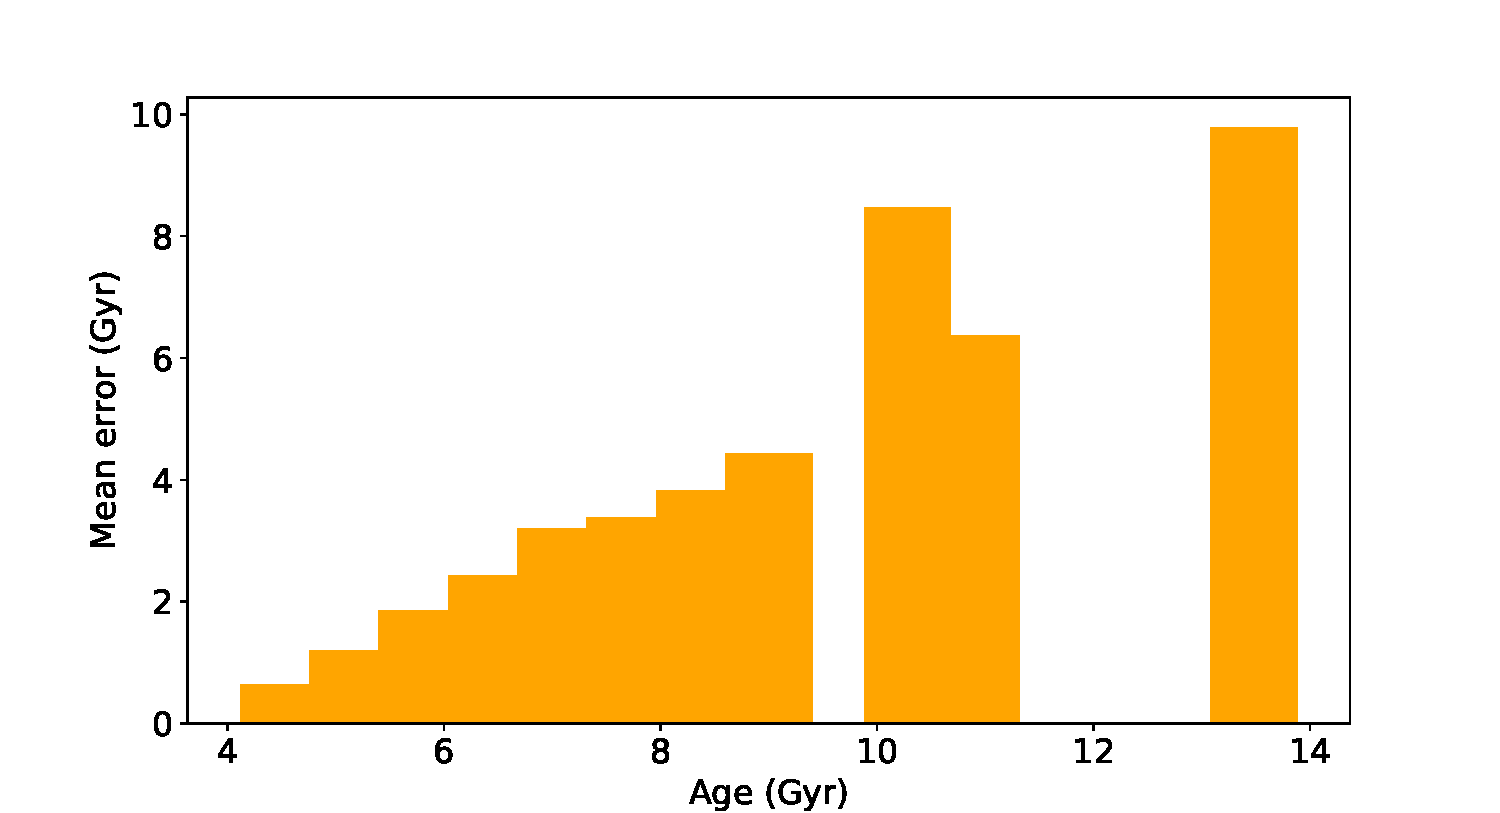
\includegraphics[width=0.8\linewidth]{Figuras/Experimentos/B_B1_nnet_3.pdf}
\end{center}
\caption{Benchmark B1: MAE en función del rango de edad del conjunto de prueba.}
 \label{fig:benchB1_best_3}
\end{figure}

\subsubsection{Benchmark B2} 

La historia es completamente diferente en el Benchmark B2. La Red Neuronal no es capaz de ser la mejor generalizando. Su error asciende hasta 1,85 Gyr, siendo superada por lr, rf, svm, knn, gp y bayes. Este último resulta ser el mejor modelo en este escenario, con un MAE de 1,48 Gyr. De la Figura \ref{fig:benchB2_best_1} y la Figura \ref{fig:benchB2_best_2} se llega a la conclusión de que un regresor bayesiano es capaz de proporcionar edades precisas en el rango de 1 Gyr a 5 Gyr, es decir, el rango cubierto por la muestra de entrenamiento en este caso. En términos de precisión, la Tabla \ref{table:precisions} revela que svm para regresión es el modelo ganador, seguido de cerca por gp y lr. El modelo bayesiano, aunque tiene el MAE más bajo, presenta una precisión del 29.71 \%.

\paragraph{Bayessian Regression} 
A continuación, se muestran las 3 gráficas que detallan el rendimiento del modelo Bayessian Regression, el cual presenta el menor MAE de este benchmark, 1.484 Gyr.

\begin{figure}[H]
\begin{center}
 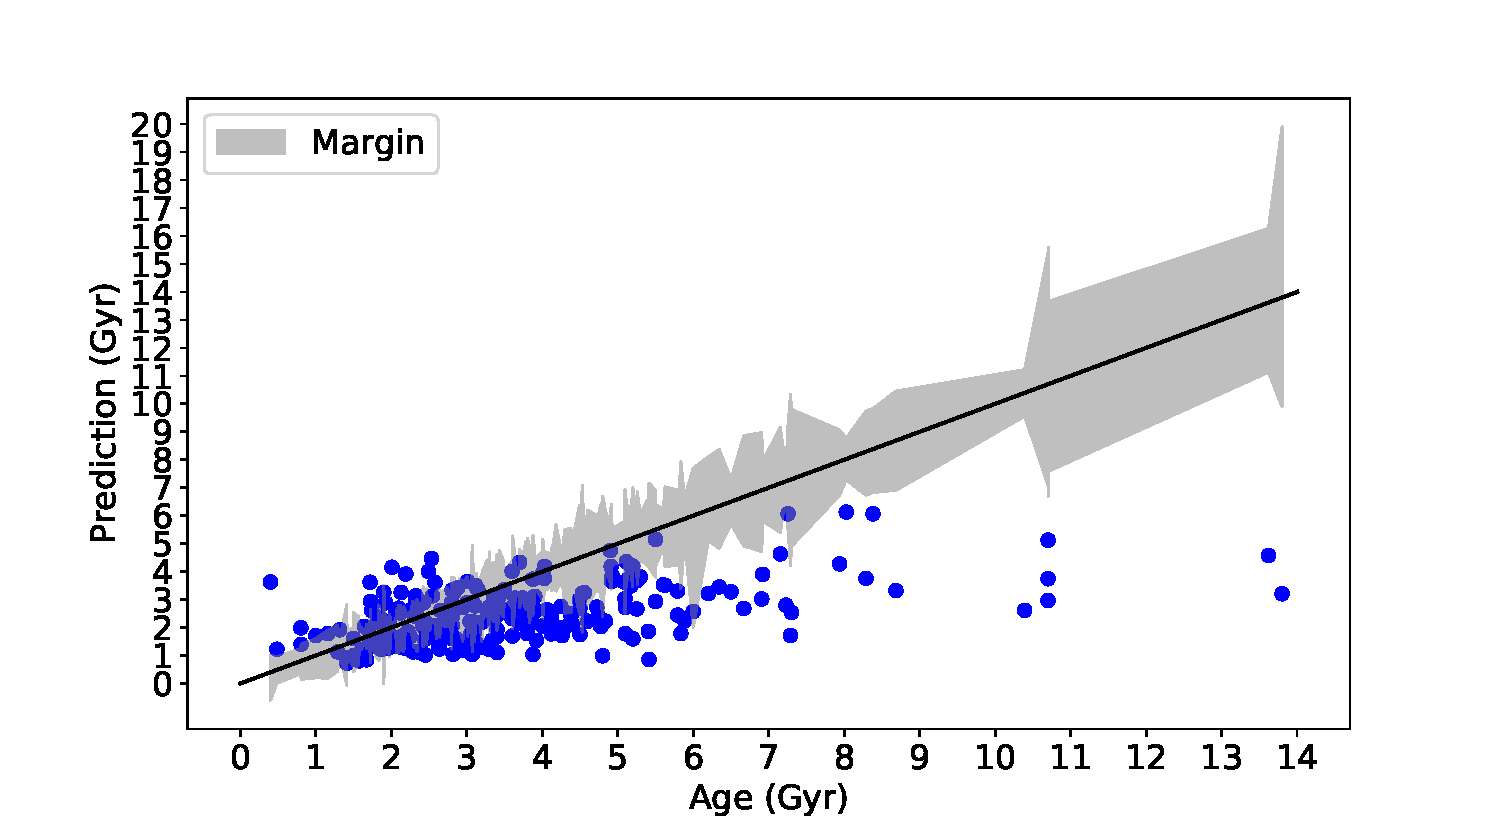
\includegraphics[width=0.8\linewidth]{Figuras/Experimentos/B_B2_bayes_1.pdf}
\end{center}
\caption{Benchmark B2: Rendimiento para el modelo Bayessian Regression.}
 \label{fig:benchB2_best_1}
\end{figure}

\begin{figure}[H]
\begin{center}
 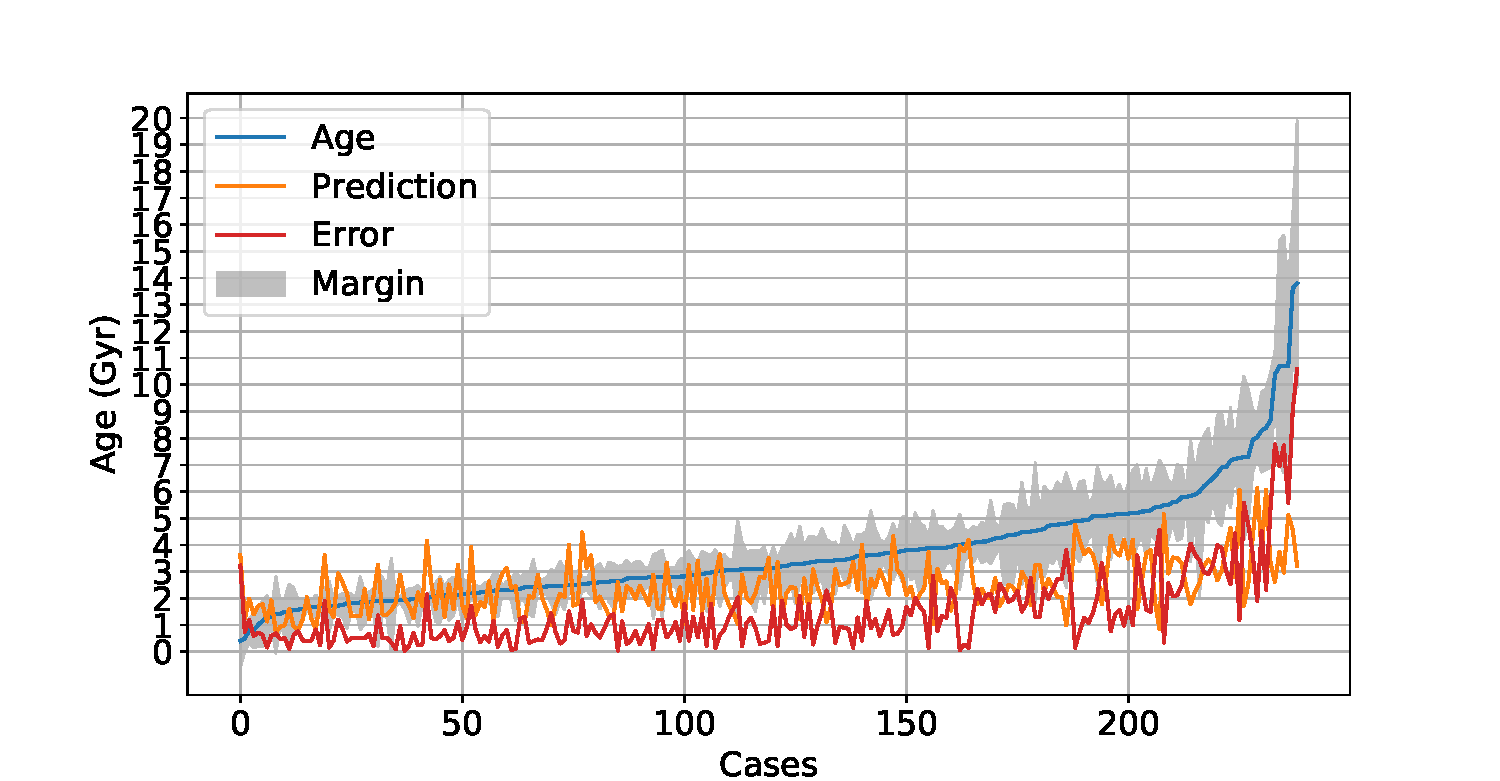
\includegraphics[width=0.8\linewidth]{Figuras/Experimentos/B_B2_bayes_2.pdf}
\end{center}
\caption{Benchmark B2: Predicción detallada para el modelo de Bayessian Regression. Se observa la edad real (en azul), la predicción de los modelos (en naranja), y el error correspondiente (en rojo).}
 \label{fig:benchB2_best_2}
\end{figure}

\begin{figure}[H]
\begin{center}
 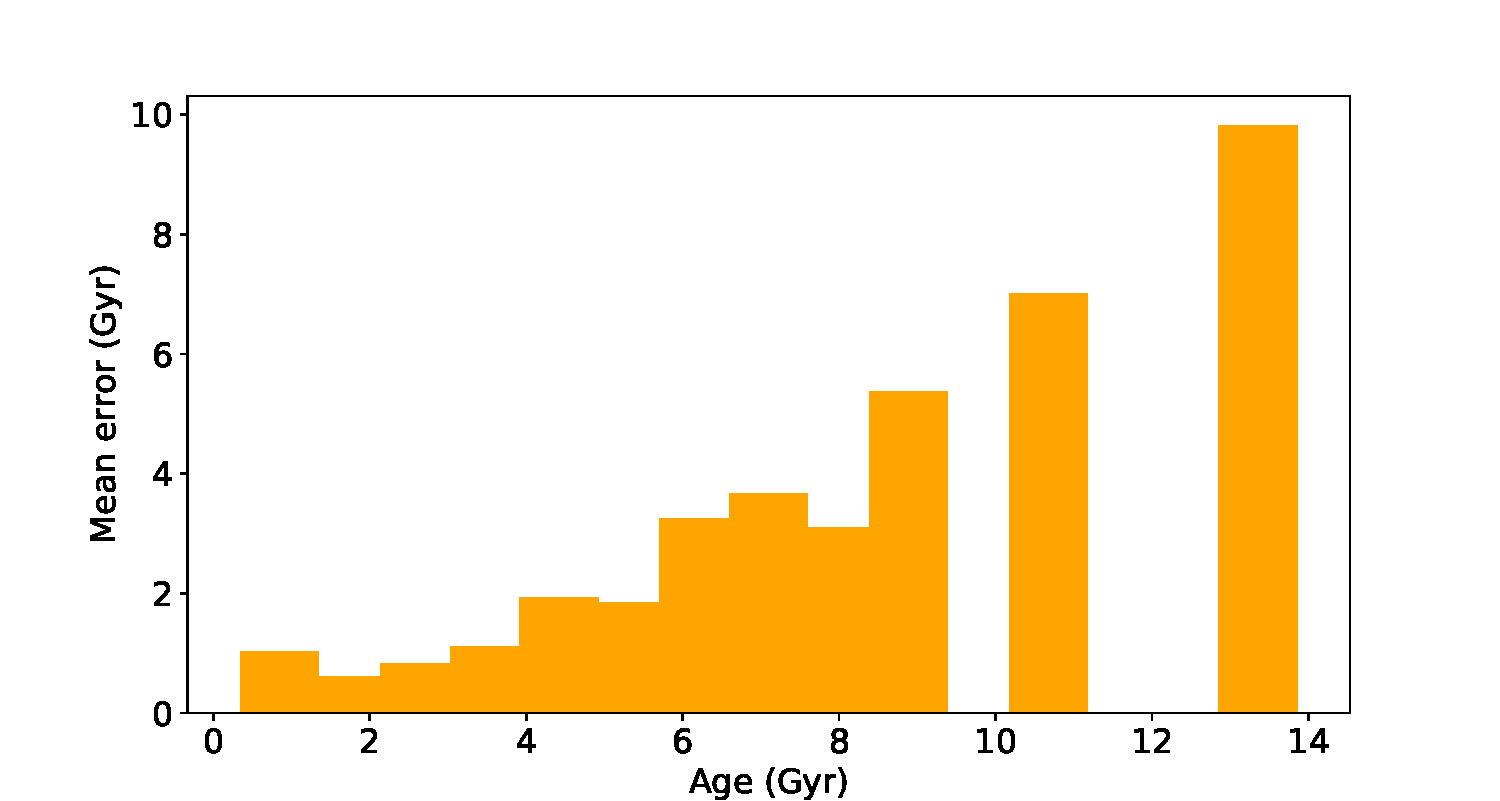
\includegraphics[width=0.8\linewidth]{Figuras/Experimentos/B_B2_bayes_3.pdf}
\end{center}
\caption{Benchmark B2: MAE en función del rango de edad del conjunto de prueba.}
 \label{fig:benchB2_best_3}
\end{figure}


Finalmente, en ambos escenarios se observa que todos los modelos tienden a subestimar las edades, aunque ese efecto es más pronunciado en el segundo Benchmark. Esto no es algo sorprendente, ya que en ambos casos las edades superiores a 4.2 Gyr no están cubiertas por las muestras de entrenamiento.

En los siguientes párrafos se muestran las figuras correspondientes al rendimiento obtenido del resto de modelos para Benchmark B1 y B2.

\paragraph{kNN} 
A continuación, se muestran las 3 gráficas que detallan el rendimiento del modelo kNN. El cual ha presentado una MAE de 1.605 Gyr.

%Benchmark B1
\begin{figure}[H]
\begin{center}
 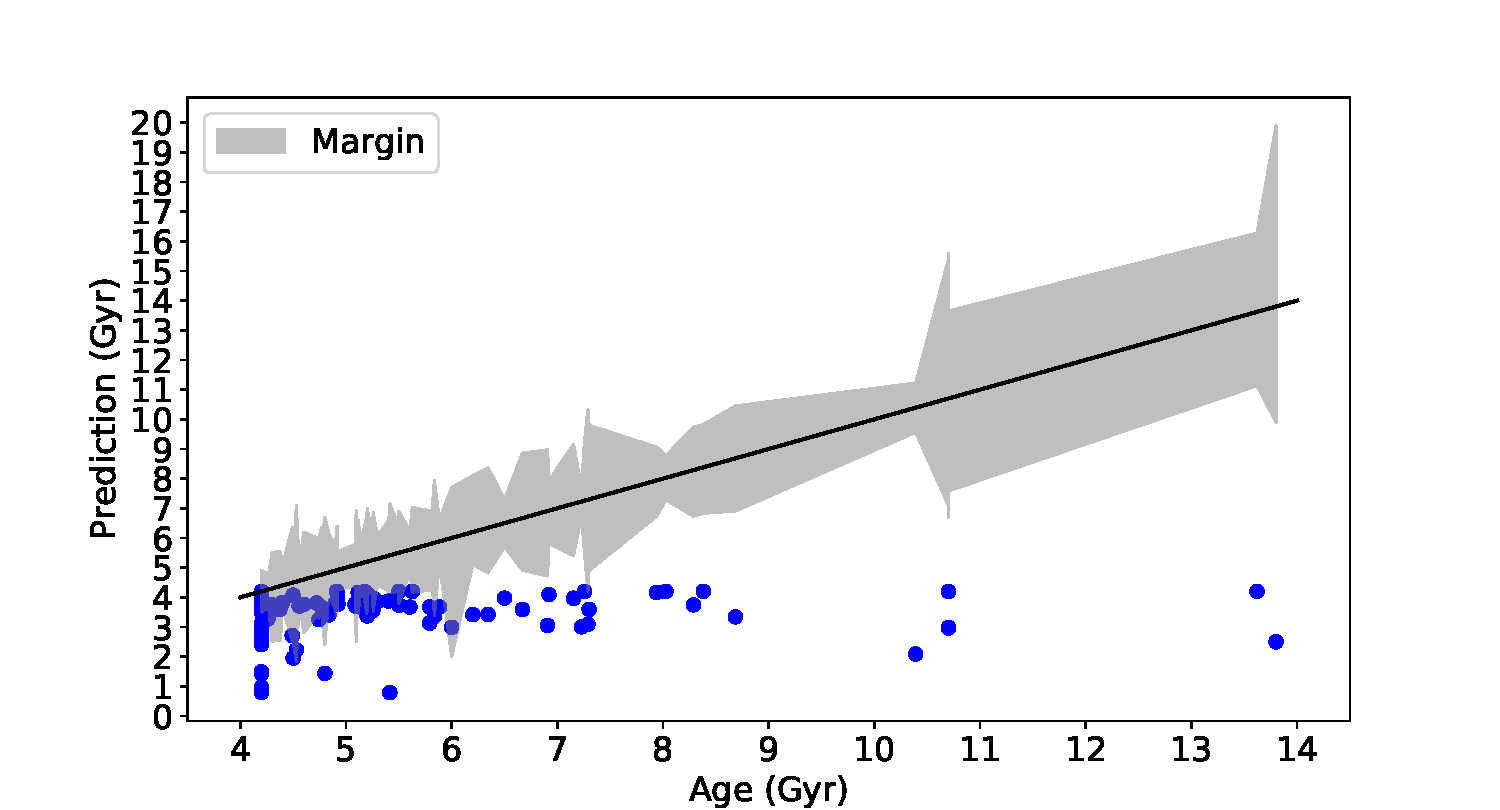
\includegraphics[width=0.8\linewidth]{Figuras/Experimentos/B_B1_knn_1.pdf}
\end{center}
\caption{Benchmark B1: Rendimiento para el modelo kNN.}
 \label{fig:benchB1_details_knn_1}
\end{figure}

\begin{figure}[H]
\begin{center}
 \includegraphics[width=0.8\linewidth]{Figuras/Experimentos/B_B1_knn_2.pdf}
\end{center}
\caption{Benchmark B1: Predicción detallada para el modelo de kNN. Se observa la edad real (en azul), la predicción de los modelos (en naranja), y el error correspondiente (en rojo).}
 \label{fig:benchB1_details_knn_2}
\end{figure}

\begin{figure}[H]
\begin{center}
 \includegraphics[width=0.8\linewidth]{Figuras/Experimentos/B_B1_knn_3.pdf}
\end{center}
\caption{Benchmark B1: MAE en función del rango de edad del conjunto de prueba.}
 \label{fig:benchB1_details_knn_3}
\end{figure}

\paragraph{Random Forest} 
A continuación, se muestran las 3 gráficas que detallan el rendimiento del modelo Random Forest. El cual ha presentado una MAE de 1.709 Gyr.

\begin{figure}[H]
\begin{center}
 \includegraphics[width=0.8\linewidth]{Figuras/Experimentos/B_B1_rf_1.pdf}
\end{center}
\caption{Benchmark B1: Rendimiento para el modelo Random Forest.}
 \label{fig:benchB1_details_rf_1}
\end{figure}

\begin{figure}[H]
\begin{center}
 \includegraphics[width=0.8\linewidth]{Figuras/Experimentos/B_B1_rf_2.pdf}
\end{center}
\caption{Benchmark B1: Predicción detallada para el modelo de Random Forest. Se observa la edad real (en azul), la predicción de los modelos (en naranja), y el error correspondiente (en rojo).}
 \label{fig:benchB1_details_rf_2}
\end{figure}

\begin{figure}[H]
\begin{center}
 \includegraphics[width=0.8\linewidth]{Figuras/Experimentos/B_B1_rf_3.pdf}
\end{center}
\caption{Benchmark B1: MAE en función del rango de edad del conjunto de prueba.}
 \label{fig:benchB1_details_rf_3}
\end{figure}

\paragraph{Support Vector Regression} 
A continuación, se muestran las 3 gráficas que detallan el rendimiento del modelo Support Vector Regression. El cual ha presentado una MAE de 1.724 Gyr.

\begin{figure}[H]
\begin{center}
 \includegraphics[width=0.8\linewidth]{Figuras/Experimentos/B_B1_svm_1.pdf}
\end{center}
\caption{Benchmark B1: Rendimiento para el modelo Support Vector Regression.}
 \label{fig:benchB1_details_svm_1}
\end{figure}

\begin{figure}[H]
\begin{center}
 \includegraphics[width=0.8\linewidth]{Figuras/Experimentos/B_B1_svm_2.pdf}
\end{center}
\caption{Benchmark B1: Predicción detallada para el modelo de Support Vector Regression. Se observa la edad real (en azul), la predicción de los modelos (en naranja), y el error correspondiente (en rojo).}
 \label{fig:benchB1_details_svm_2}
\end{figure}

\begin{figure}[H]
\begin{center}
 \includegraphics[width=0.8\linewidth]{Figuras/Experimentos/B_B1_svm_3.pdf}
\end{center}
\caption{Benchmark B1: MAE en función del rango de edad del conjunto de prueba.}
 \label{fig:benchB1_details_svm_3}
\end{figure}

\paragraph{Decision Tree Regression} 
A continuación, se muestran las 3 gráficas que detallan el rendimiento del modelo Decision Tree Regression. El cual ha presentado una MAE de 1.621 Gyr.

\begin{figure}[H]
\begin{center}
 \includegraphics[width=0.8\linewidth]{Figuras/Experimentos/B_B1_dtr_1.pdf}
\end{center}
\caption{Benchmark B1: Rendimiento para el modelo Decision Tree Regression.}
 \label{fig:benchB1_details_dtr_1}
\end{figure}

\begin{figure}[H]
\begin{center}
 \includegraphics[width=0.8\linewidth]{Figuras/Experimentos/B_B1_dtr_2.pdf}
\end{center}
\caption{Benchmark B1: Predicción detallada para el modelo de Decision Tree Regression. Se observa la edad real (en azul), la predicción de los modelos (en naranja), y el error correspondiente (en rojo).}
 \label{fig:benchB1_details_dtr_2}
\end{figure}

\begin{figure}[H]
\begin{center}
 \includegraphics[width=0.8\linewidth]{Figuras/Experimentos/B_B1_dtr_3.pdf}
\end{center}
\caption{Benchmark B1: MAE en función del rango de edad del conjunto de prueba.}
 \label{fig:benchB1_details_dtr_3}
\end{figure}

\paragraph{Linear Regressor} 
A continuación, se muestran las 3 gráficas que detallan el rendimiento del modelo Linear Regressor. El cual ha presentado una MAE de 1.923 Gyr.

\begin{figure}[H]
\begin{center}
 \includegraphics[width=0.8\linewidth]{Figuras/Experimentos/B_B1_lr_1.pdf}
\end{center}
\caption{Benchmark B1: Rendimiento para el modelo Linear Regressor.}
 \label{fig:benchB1_details_lr_1}
\end{figure}

\begin{figure}[H]
\begin{center}
 \includegraphics[width=0.8\linewidth]{Figuras/Experimentos/B_B1_lr_2.pdf}
\end{center}
\caption{Benchmark B1: Predicción detallada para el modelo de Linear Regressor. Se observa la edad real (en azul), la predicción de los modelos (en naranja), y el error correspondiente (en rojo).}
 \label{fig:benchB1_details_lr_2}
\end{figure}

\begin{figure}[H]
\begin{center}
 \includegraphics[width=0.8\linewidth]{Figuras/Experimentos/B_B1_lr_3.pdf}
\end{center}
\caption{Benchmark B1: MAE en función del rango de edad del conjunto de prueba.}
 \label{fig:benchB1_details_lr_3}
\end{figure}

\paragraph{Bayesian Regression} 
A continuación, se muestran las 3 gráficas que detallan el rendimiento del modelo Bayesian Regression. El cual ha presentado una MAE de 1.943 Gyr.

\begin{figure}[H]
\begin{center}
 \includegraphics[width=0.8\linewidth]{Figuras/Experimentos/B_B1_bayes_1.pdf}
\end{center}
\caption{Benchmark B1: Rendimiento para el modelo Bayesian Regression.}
 \label{fig:benchB1_details_bayes_1}
\end{figure}

\begin{figure}[H]
\begin{center}
 \includegraphics[width=0.8\linewidth]{Figuras/Experimentos/B_B1_bayes_2.pdf}
\end{center}
\caption{Benchmark B1: Predicción detallada para el modelo de Bayesian Regression. Se observa la edad real (en azul), la predicción de los modelos (en naranja), y el error correspondiente (en rojo).}
 \label{fig:benchB1_details_bayes_2}
\end{figure}

\begin{figure}[H]
\begin{center}
 \includegraphics[width=0.8\linewidth]{Figuras/Experimentos/B_B1_bayes_3.pdf}
\end{center}
\caption{Benchmark B1: MAE en función del rango de edad del conjunto de prueba.}
 \label{fig:benchB1_details_bayes_3}
\end{figure}

\paragraph{Gaussian Process} 
A continuación, se muestran las 3 gráficas que detallan el rendimiento del modelo Gaussian Process. El cual ha presentado una MAE de 1.670 Gyr.

\begin{figure}[H]
\begin{center}
 \includegraphics[width=0.8\linewidth]{Figuras/Experimentos/B_B1_gp_1.pdf}
\end{center}
\caption{Benchmark B1: Rendimiento para el modelo Gaussian Process.}
 \label{fig:benchB1_details_gp_1}
\end{figure}

\begin{figure}[H]
\begin{center}
 \includegraphics[width=0.8\linewidth]{Figuras/Experimentos/B_B1_gp_2.pdf}
\end{center}
\caption{Benchmark B1: Predicción detallada para el modelo de Gaussian Process. Se observa la edad real (en azul), la predicción de los modelos (en naranja), y el error correspondiente (en rojo).}
 \label{fig:benchB1_details_gp_2}
\end{figure}

\begin{figure}[H]
\begin{center}
 \includegraphics[width=0.8\linewidth]{Figuras/Experimentos/B_B1_gp_3.pdf}
\end{center}
\caption{Benchmark B1: MAE en función del rango de edad del conjunto de prueba.}
 \label{fig:benchB1_details_gp_3}
\end{figure}

%Benchmark B2
\paragraph{kNN} 
A continuación, se muestran las 3 gráficas que detallan el rendimiento del modelo kNN. El cual ha presentado una MAE de 1.841 Gyr.

\begin{figure}[H]
\begin{center}
 \includegraphics[width=0.8\linewidth]{Figuras/Experimentos/B_B2_knn_1.pdf}
\end{center}
\caption{Benchmark B2: Rendimiento para el modelo kNN.}
 \label{fig:benchB2_details_knn_1}
\end{figure}

\begin{figure}[H]
\begin{center}
 \includegraphics[width=0.8\linewidth]{Figuras/Experimentos/B_B2_knn_2.pdf}
\end{center}
\caption{Benchmark B2: Predicción detallada para el modelo de kNN. Se observa la edad real (en azul), la predicción de los modelos (en naranja), y el error correspondiente (en rojo).}
 \label{fig:benchB2_details_knn_2}
\end{figure}

\begin{figure}[H]
\begin{center}
 \includegraphics[width=0.8\linewidth]{Figuras/Experimentos/B_B2_knn_3.pdf}
\end{center}
\caption{Benchmark B2: MAE en función del rango de edad del conjunto de prueba.}
 \label{fig:benchB2_details_knn_3}
\end{figure}

\paragraph{Random Forest} 
A continuación, se muestran las 3 gráficas que detallan el rendimiento del modelo Random Forest. El cual ha presentado una MAE de 1.852 Gyr.

\begin{figure}[H]
\begin{center}
 \includegraphics[width=0.8\linewidth]{Figuras/Experimentos/B_B2_rf_1.pdf}
\end{center}
\caption{Benchmark B2: Rendimiento para el modelo Random Forest.}
 \label{fig:benchB2_details_rf_1}
\end{figure}

\begin{figure}[H]
\begin{center}
 \includegraphics[width=0.8\linewidth]{Figuras/Experimentos/B_B2_rf_2.pdf}
\end{center}
\caption{Benchmark B2: Predicción detallada para el modelo de Random Forest. Se observa la edad real (en azul), la predicción de los modelos (en naranja), y el error correspondiente (en rojo).}
 \label{fig:benchB2_details_rf_2}
\end{figure}

\begin{figure}[H]
\begin{center}
 \includegraphics[width=0.8\linewidth]{Figuras/Experimentos/B_B2_rf_3.pdf}
\end{center}
\caption{Benchmark B2: MAE en función del rango de edad del conjunto de prueba.}
 \label{fig:benchB2_details_rf_3}
\end{figure}

\paragraph{Support Vector Regression} 
A continuación, se muestran las 3 gráficas que detallan el rendimiento del modelo Support Vector Regression. El cual ha presentado una MAE de 1.507 Gyr.

\begin{figure}[H]
\begin{center}
 \includegraphics[width=0.8\linewidth]{Figuras/Experimentos/B_B2_svm_1.pdf}
\end{center}
\caption{Benchmark B2: Rendimiento para el modelo Support Vector Regression.}
 \label{fig:benchB2_details_svm_1}
\end{figure}

\begin{figure}[H]
\begin{center}
 \includegraphics[width=0.8\linewidth]{Figuras/Experimentos/B_B2_svm_2.pdf}
\end{center}
\caption{Benchmark B2: Predicción detallada para el modelo de Support Vector Regression. Se observa la edad real (en azul), la predicción de los modelos (en naranja), y el error correspondiente (en rojo).}
 \label{fig:benchB2_details_svm_2}
\end{figure}

\begin{figure}[H]
\begin{center}
 \includegraphics[width=0.8\linewidth]{Figuras/Experimentos/B_B2_svm_3.pdf}
\end{center}
\caption{Benchmark B2: MAE en función del rango de edad del conjunto de prueba.}
 \label{fig:benchB2_details_svm_3}
\end{figure}

\paragraph{Decision Tree Regression} 
A continuación, se muestran las 3 gráficas que detallan el rendimiento del modelo Decision Tree Regression. El cual ha presentado una MAE de 1.901 Gyr.

\begin{figure}[H]
\begin{center}
 \includegraphics[width=0.8\linewidth]{Figuras/Experimentos/B_B2_dtr_1.pdf}
\end{center}
\caption{Benchmark B2: Rendimiento para el modelo Decision Tree Regression.}
 \label{fig:benchB2_details_dtr_1}
\end{figure}

\begin{figure}[H]
\begin{center}
 \includegraphics[width=0.8\linewidth]{Figuras/Experimentos/B_B2_dtr_2.pdf}
\end{center}
\caption{Benchmark B2: Predicción detallada para el modelo de Decision Tree Regression. Se observa la edad real (en azul), la predicción de los modelos (en naranja), y el error correspondiente (en rojo).}
 \label{fig:benchB2_details_dtr_2}
\end{figure}

\begin{figure}[H]
\begin{center}
 \includegraphics[width=0.8\linewidth]{Figuras/Experimentos/B_B2_dtr_3.pdf}
\end{center}
\caption{Benchmark B2: MAE en función del rango de edad del conjunto de prueba.}
 \label{fig:benchB2_details_dtr_3}
\end{figure}

\paragraph{Linear Regressor} 
A continuación, se muestran las 3 gráficas que detallan el rendimiento del modelo Linear Regressor. El cual ha presentado una MAE de 1.561 Gyr.

\begin{figure}[H]
\begin{center}
 \includegraphics[width=0.8\linewidth]{Figuras/Experimentos/B_B2_lr_1.pdf}
\end{center}
\caption{Benchmark B2: Rendimiento para el modelo Linear Regressor.}
 \label{fig:benchB2_details_lr_1}
\end{figure}

\begin{figure}[H]
\begin{center}
 \includegraphics[width=0.8\linewidth]{Figuras/Experimentos/B_B2_lr_2.pdf}
\end{center}
\caption{Benchmark B2: Predicción detallada para el modelo de Linear Regressor. Se observa la edad real (en azul), la predicción de los modelos (en naranja), y el error correspondiente (en rojo).}
 \label{fig:benchB2_details_lr_2}
\end{figure}

\begin{figure}[H]
\begin{center}
 \includegraphics[width=0.8\linewidth]{Figuras/Experimentos/B_B2_lr_3.pdf}
\end{center}
\caption{Benchmark B2: MAE en función del rango de edad del conjunto de prueba.}
 \label{fig:benchB2_details_lr_3}
\end{figure}

\paragraph{Neural Network} 
A continuación, se muestran las 3 gráficas que detallan el rendimiento del modelo Neural Network. El cual ha presentado una MAE de 1.853 Gyr.

\begin{figure}[H]
\begin{center}
 \includegraphics[width=0.8\linewidth]{Figuras/Experimentos/B_B2_nnet_1.pdf}
\end{center}
\caption{Benchmark B2: Rendimiento para el modelo Neural Network.}
 \label{fig:benchB2_details_nnet_1}
\end{figure}

\begin{figure}[H]
\begin{center}
 \includegraphics[width=0.8\linewidth]{Figuras/Experimentos/B_B2_nnet_2.pdf}
\end{center}
\caption{Benchmark B2: Predicción detallada para el modelo de Neural Network. Se observa la edad real (en azul), la predicción de los modelos (en naranja), y el error correspondiente (en rojo).}
 \label{fig:benchB2_details_nnet_2}
\end{figure}

\begin{figure}[H]
\begin{center}
 \includegraphics[width=0.8\linewidth]{Figuras/Experimentos/B_B2_nnet_3.pdf}
\end{center}
\caption{Benchmark B2: MAE en función del rango de edad del conjunto de prueba.}
 \label{fig:benchB2_details_nnet_3}
\end{figure}

\paragraph{Gaussian Process} 
A continuación, se muestran las 3 gráficas que detallan el rendimiento del modelo Gaussian Process. El cual ha presentado una MAE de 1.624 Gyr.

\begin{figure}[H]
\begin{center}
 \includegraphics[width=0.8\linewidth]{Figuras/Experimentos/B_B2_gp_1.pdf}
\end{center}
\caption{Benchmark B2: Rendimiento para el modelo Gaussian Process.}
 \label{fig:benchB2_details_gp_1}
\end{figure}

\begin{figure}[H]
\begin{center}
 \includegraphics[width=0.8\linewidth]{Figuras/Experimentos/B_B2_gp_2.pdf}
\end{center}
\caption{Benchmark B2: Predicción detallada para el modelo de Gaussian Process. Se observa la edad real (en azul), la predicción de los modelos (en naranja), y el error correspondiente (en rojo).}
 \label{fig:benchB2_details_gp_2}
\end{figure}

\begin{figure}[H]
\begin{center}
 \includegraphics[width=0.8\linewidth]{Figuras/Experimentos/B_B2_gp_3.pdf}
\end{center}
\caption{Benchmark B2: MAE en función del rango de edad del conjunto de prueba.}
 \label{fig:benchB2_details_gp_3}
\end{figure}


\subsection{Benchmark C: Rendimiento sobre la muestra de control}

Se muestra el MAE y la precisión para cada método para el Benchmark de control en la Figura \ref{fig:benchC} y en la Tabla \ref{table:precisions}, respectivamente. En esta ocasión, los tres mejores métodos son gp, nnet y su Stacking. Entre estos tres, descata el proceso gaussiano. En la Figura \ref{fig:benchC_best_1} y Figura \ref{fig:benchC_best_2} se pueden inspeccionar las predicciones de las edades estelares usando este método frente a las edades de referencia para las estrellas de ese set. gp es el modelo con mayor precisión: $40.62\%$ de las predicciones caen dentro del margen de confianza del conjunto de datos. Para el Sol, gp predice una edad de 3,88 Gys frente a una edad aceptada de 4,6 Gyr, subestimándola. De hecho, el modelo tiende a subestimar ligeramente la mayoría de las edades. Se observa este comportamiento en todos lo modelos salvo en kNN y dtr. 

\begin{figure}[H]
\begin{center}
 \includegraphics[width=0.8\linewidth]{Figuras/Experimentos/B_C_models.pdf}
\end{center}
\caption{Benchmark C: Rendimiento de los modelos en función del MAE.}
 \label{fig:benchC}
\end{figure}

%Precision for the SUN
Respecto a la precisión en las estimaciones para la edad del Sol, 4,6 Gyr, se proporciona en la Tabla \ref{table:sun_results} la edad específica obtenida en cada uno de los modelos. Todos los métodos subestiman, y rf obtiene la predicción más cercana, seguido de dtr y kNN.


\begin{table}[H]
\centering
\scalebox{0.6}{
\begin{tabular}{l|ccccccccc}  
\toprule
\textbf{Métodos}  & nnet & lr & dtr & rf & svm & bayes & knn & gp & stacking \\
\midrule
Sol (4.6 Gyr)  & 4.02 & 3.92 & 4.49 & 4.76 & 3.81 & 3.91 & 4.49 & 3.88 & 4.02\\
\bottomrule
\end{tabular}
}%end of scalebox
\caption{Edad estimada para el Sol en Gyr. El método más preciso es rf. }\label{table:sun_results}
\end{table}

\paragraph{Gaussian Process} 
A continuación, se muestran las 3 gráficas que detallan el rendimiento del modelo Gaussian Process. El mejor modelo en este benchmark, con un MAE de 0.837 Gyr.

\begin{figure}[H]
\begin{center}
 \includegraphics[width=0.8\linewidth]{Figuras/Experimentos/B_C_gp_1.pdf}
\end{center}
\caption{Benchmark C: Rendimiento para el modelo Gaussian Process. El punto amarillo se corresponde con la representación de la estimación de la edad del Sol.}
 \label{fig:benchC_best_1}
\end{figure}

\begin{figure}[H]
\begin{center}
 \includegraphics[width=0.8\linewidth]{Figuras/Experimentos/B_C_gp_2.pdf}
\end{center}
\caption{Benchmark C: Predicción detallada para el modelo de Gaussian Process. Se observa la edad real (en azul), la predicción de los modelos (en naranja), y el error correspondiente (en rojo).El punto amarillo se corresponde con la representación de la estimación de la edad del Sol.}
 \label{fig:benchC_best_2}
\end{figure}

\begin{figure}[H]
\begin{center}
 \includegraphics[width=0.8\linewidth]{Figuras/Experimentos/B_C_gp_3.pdf}
\end{center}
\caption{Benchmark C: MAE en función del rango de edad del conjunto de prueba.}
 \label{fig:benchC_best_3}
\end{figure}


\paragraph{Stacking} 
A continuación, se muestran las 3 gráficas que detallan el rendimiento del modelo Stacking. El cual ha presentado un MAE de 0.991 Gyr.

\begin{figure}[H]
\begin{center}
 \includegraphics[width=0.8\linewidth]{Figuras/Experimentos/B_C_stacking_1.pdf}
\end{center}
\caption{Benchmark C: Rendimiento para el modelo Stacking. El punto amarillo se corresponde con la representación de la estimación de la edad del Sol.}
 \label{fig:benchC_details_stacking_1}
\end{figure}

\begin{figure}[H]
\begin{center}
 \includegraphics[width=0.8\linewidth]{Figuras/Experimentos/B_C_stacking_2.pdf}
\end{center}
\caption{Benchmark C: Predicción detallada para el modelo de Stacking. Se observa la edad real (en azul), la predicción de los modelos (en naranja), y el error correspondiente (en rojo). El punto amarillo se corresponde con la representación de la estimación de la edad del Sol.}
 \label{fig:benchC_details_stacking_2}
\end{figure}

\begin{figure}[H]
\begin{center}
 \includegraphics[width=0.8\linewidth]{Figuras/Experimentos/B_C_stacking_3.pdf}
\end{center}
\caption{Benchmark C: MAE en función del rango de edad del conjunto de prueba.}
 \label{fig:benchC_details_stacking_3}
\end{figure}

\paragraph{Neural Network} 
A continuación, se muestran las 3 gráficas que detallan el rendimiento del modelo Neural Network. El cual ha presentado un MAE de 1.098 Gyr.

\begin{figure}[H]
\begin{center}
 \includegraphics[width=0.8\linewidth]{Figuras/Experimentos/B_C_nnet_1.pdf}
\end{center}
\caption{Benchmark C: Rendimiento para el modelo Neural Network. El punto amarillo se corresponde con la representación de la estimación de la edad del Sol.}
 \label{fig:benchC_details_nnet_1}
\end{figure}

\begin{figure}[H]
\begin{center}
 \includegraphics[width=0.8\linewidth]{Figuras/Experimentos/B_C_nnet_2.pdf}
\end{center}
\caption{Benchmark C: Predicción detallada para el modelo de la Neural Network. Se observa la edad real (en azul), la predicción de los modelos (en naranja), y el error correspondiente (en rojo). El punto amarillo se corresponde con la representación de la estimación de la edad del Sol.}
 \label{fig:benchC_details_nnet_2}
\end{figure}

\begin{figure}[H]
\begin{center}
 \includegraphics[width=0.8\linewidth]{Figuras/Experimentos/B_C_nnet_3.pdf}
\end{center}
\caption{Benchmark C: MAE en función del rango de edad del conjunto de prueba.}
 \label{fig:benchC_details_nnet_3}
\end{figure}

\paragraph{kNN} 
A continuación, se muestran las 3 gráficas que detallan el rendimiento del modelo kNN. El cual ha presentado un MAE de 1.734 Gyr.

\begin{figure}[H]
\begin{center}
 \includegraphics[width=0.8\linewidth]{Figuras/Experimentos/B_C_knn_1.pdf}
\end{center}
\caption{Benchmark C: Rendimiento para el modelo kNN. El punto amarillo se corresponde con la representación de la estimación de la edad del Sol.}
 \label{fig:benchC_details_knn_1}
\end{figure}

\begin{figure}[H]
\begin{center}
 \includegraphics[width=0.8\linewidth]{Figuras/Experimentos/B_C_knn_2.pdf}
\end{center}
\caption{Benchmark C: Predicción detallada para el modelo de kNN. Se observa la edad real (en azul), la predicción de los modelos (en naranja), y el error correspondiente (en rojo). El punto amarillo se corresponde con la representación de la estimación de la edad del Sol.}
 \label{fig:benchC_details_knn_2}
\end{figure}

\begin{figure}[H]
\begin{center}
 \includegraphics[width=0.8\linewidth]{Figuras/Experimentos/B_C_knn_3.pdf}
\end{center}
\caption{Benchmark C: MAE en función del rango de edad del conjunto de prueba.}
 \label{fig:benchC_details_knn_3}
\end{figure}

\paragraph{Random Forest} 
A continuación, se muestran las 3 gráficas que detallan el rendimiento del modelo Random Forest. El cual ha presentado un MAE de 1.006 Gyr.

\begin{figure}[H]
\begin{center}
 \includegraphics[width=0.8\linewidth]{Figuras/Experimentos/B_C_rf_1.pdf}
\end{center}
\caption{Benchmark C: Rendimiento para el modelo Random Forest. El punto amarillo se corresponde con la representación de la estimación de la edad del Sol.}
 \label{fig:benchC_details_rf_1}
\end{figure}

\begin{figure}[H]
\begin{center}
 \includegraphics[width=0.8\linewidth]{Figuras/Experimentos/B_C_rf_2.pdf}
\end{center}
\caption{Benchmark C: Predicción detallada para el modelo de Random Forest. Se observa la edad real (en azul), la predicción de los modelos (en naranja), y el error correspondiente (en rojo). El punto amarillo se corresponde con la representación de la estimación de la edad del Sol.}
 \label{fig:benchC_details_rf_2}
\end{figure}

\begin{figure}[H]
\begin{center}
 \includegraphics[width=0.8\linewidth]{Figuras/Experimentos/B_C_rf_3.pdf}
\end{center}
\caption{Benchmark C: MAE en función del rango de edad del conjunto de prueba.}
 \label{fig:benchC_details_rf_3}
\end{figure}

\paragraph{Support Vector Regression} 
A continuación, se muestran las 3 gráficas que detallan el rendimiento del modelo Support Vector Regression. El cual ha presentado un MAE de 1.278 Gyr.

\begin{figure}[H]
\begin{center}
 \includegraphics[width=0.8\linewidth]{Figuras/Experimentos/B_C_svm_1.pdf}
\end{center}
\caption{Benchmark C: Rendimiento para el modelo Support Vector Regression. El punto amarillo se corresponde con la representación de la estimación de la edad del Sol.}
 \label{fig:benchC_details_svm_1}
\end{figure}

\begin{figure}[H]
\begin{center}
 \includegraphics[width=0.8\linewidth]{Figuras/Experimentos/B_C_svm_2.pdf}
\end{center}
\caption{Benchmark C: Predicción detallada para el modelo de Support Vector Regression. Se observa la edad real (en azul), la predicción de los modelos (en naranja), y el error correspondiente (en rojo). El punto amarillo se corresponde con la representación de la estimación de la edad del Sol.}
 \label{fig:benchC_details_svm_2}
\end{figure}

\begin{figure}[H]
\begin{center}
 \includegraphics[width=0.8\linewidth]{Figuras/Experimentos/B_C_svm_3.pdf}
\end{center}
\caption{Benchmark C: MAE en función del rango de edad del conjunto de prueba.}
 \label{fig:benchC_details_svm_3}
\end{figure}

\paragraph{Decision Tree Regression} 
A continuación, se muestran las 3 gráficas que detallan el rendimiento del modelo Decision Tree Regression. El cual ha presentado un MAE de 2.113 Gyr.

\begin{figure}[H]
\begin{center}
 \includegraphics[width=0.8\linewidth]{Figuras/Experimentos/B_C_dtr_1.pdf}
\end{center}
\caption{Benchmark C: Rendimiento para el modelo Decision Tree Regression. El punto amarillo se corresponde con la representación de la estimación de la edad del Sol.}
 \label{fig:benchC_details_dtr_1}
\end{figure}

\begin{figure}[H]
\begin{center}
 \includegraphics[width=0.8\linewidth]{Figuras/Experimentos/B_C_dtr_2.pdf}
\end{center}
\caption{Benchmark C: Predicción detallada para el modelo de Decision Tree Regression. Se observa la edad real (en azul), la predicción de los modelos (en naranja), y el error correspondiente (en rojo). El punto amarillo se corresponde con la representación de la estimación de la edad del Sol.}
 \label{fig:benchC_details_dtr_2}
\end{figure}

\begin{figure}[H]
\begin{center}
 \includegraphics[width=0.8\linewidth]{Figuras/Experimentos/B_C_dtr_3.pdf}
\end{center}
\caption{Benchmark C: MAE en función del rango de edad del conjunto de prueba.}
 \label{fig:benchC_details_dtr_3}
\end{figure}

\paragraph{Linear Regressor} 
A continuación, se muestran las 3 gráficas que detallan el rendimiento del modelo Linear Regressor. El cual ha presentado un MAE de 1.297 Gyr.

\begin{figure}[H]
\begin{center}
 \includegraphics[width=0.8\linewidth]{Figuras/Experimentos/B_C_lr_1.pdf}
\end{center}
\caption{Benchmark C: Rendimiento para el modelo Linear Regressor. El punto amarillo se corresponde con la representación de la estimación de la edad del Sol.}
 \label{fig:benchC_details_lr_1}
\end{figure}

\begin{figure}[H]
\begin{center}
 \includegraphics[width=0.8\linewidth]{Figuras/Experimentos/B_C_lr_2.pdf}
\end{center}
\caption{Benchmark C: Predicción detallada para el modelo de Linear Regressor. Se observa la edad real (en azul), la predicción de los modelos (en naranja), y el error correspondiente (en rojo). El punto amarillo se corresponde con la representación de la estimación de la edad del Sol.}
 \label{fig:benchC_details_lr_2}
\end{figure}

\begin{figure}[H]
\begin{center}
 \includegraphics[width=0.8\linewidth]{Figuras/Experimentos/B_C_lr_3.pdf}
\end{center}
\caption{Benchmark C: MAE en función del rango de edad del conjunto de prueba.}
 \label{fig:benchC_details_lr_3}
\end{figure}

\paragraph{Bayesian Regression} 
A continuación, se muestran las 3 gráficas que detallan el rendimiento del modelo Bayesian Regression. El cual ha presentado un MAE de 1.297 Gyr.

\begin{figure}[H]
\begin{center}
 \includegraphics[width=0.8\linewidth]{Figuras/Experimentos/B_C_bayes_1.pdf}
\end{center}
\caption{Benchmark C: Rendimiento para el modelo Bayesian Regression. El punto amarillo se corresponde con la representación de la estimación de la edad del Sol.}
 \label{fig:benchC_details_bayes_1}
\end{figure}

\begin{figure}[H]
\begin{center}
 \includegraphics[width=0.8\linewidth]{Figuras/Experimentos/B_C_bayes_2.pdf}
\end{center}
\caption{Benchmark C: Predicción detallada para el modelo de Bayesian Regression. Se observa la edad real (en azul), la predicción de los modelos (en naranja), y el error correspondiente (en rojo). El punto amarillo se corresponde con la representación de la estimación de la edad del Sol.}
 \label{fig:benchC_details_bayes_2}
\end{figure}

\begin{figure}[H]
\begin{center}
 \includegraphics[width=0.8\linewidth]{Figuras/Experimentos/B_C_bayes_3.pdf}
\end{center}
\caption{Benchmark C: MAE en función del rango de edad del conjunto de prueba.}
 \label{fig:benchC_details_bayes_3}
\end{figure}

\subsection{Conclusiones de la comparativa}

Comparando los resultados de los Benchmark A (Figura \ref{fig:benchA_models}) y C (Figura \ref{fig:benchC}), se puede concluir que: a) los modelos ganadores son comunes (nnet, gp y stacking); b) kNN y dtr sufren una degración considerable de su rendimiento, ya que dependen en gran medida de la distribución de datos utilizada durante su entrenamiento; y c) bayes y lr son similares, mostrando un incremento similar en sus correspondientes MAEs, pero al mismo tiempo ofreciendo cierta estabilidad entre escenarios.

Al observar la Tabla \ref{table:precisions} después de conocer el rendimiento de todos los modelos, además de lo comentado en cada uno de los benchmarks, se llega a la conclusión de que: a) salvo para el Benchmark B2, nnet presenta una precisión alta en comparación con el resto de modelos y b) salvo para el Benchmark B2, lr y bayes presentan una precisión muy inferior a la conseguida por el modelo de mejor rendimiento.

\begin{table}[H]
\centering
\scalebox{0.6}{
\begin{tabular}{l|ccccccccc}  
\toprule
Benchmark & nnet & lr & dtr & rf & svm & bayes & knn & gp & stacking \\
\midrule
\textbf{A}  & 73.23 & 35.43 & 63.78 & 60.63 & 46.46 & 32.28 & \textbf{77.95} & 62.20 & 62.99\\
\textbf{B1}  & \textbf{59.84} & 29.92 & 51.18 & 48.03 & 37.79 & 28.35 & 55.91 & 51.97 & n/a \\
\textbf{B2}  & 28.45 & 30.96 & 21.34 & 25.94 & \textbf{33.05} & 29.71 & 25.52 & 30.96 & n/a\\
\textbf{C}  & 34.37 & 21.87 & 9.37 & 21.87 & 12.50 & 21.87 & 15.62 & \textbf{40.62} & 34.37\\
\bottomrule
\end{tabular}
}%end of scalebox
\caption{Precisión de todos los métodos en los diferentes benchmarks. La precisión se mide como el porcentaje de estimaciones de edad que caen dentro del margen de confianza asociado a cada estrella.}\label{table:precisions}
\end{table}


\chapter{Continual learning}
 
\section{Introducción}

En este trabajo, además de realizar un estudio comparativo sobre los modelos tradicionales de Inteligencia Artificial, se estudia la aplicación del algoritmo MAML (model-agnostic meta-learning) para el problema de la estimación de edades estelares. Este algoritmo se denomina agnóstico del modelo porque es compatible con cualquier modelo entrenado con descenso de gradiente y aplicable a una variedad de diferentes problemas de aprendizaje, incluyendo clasificación, regresión y aprendizaje por refuerzo. El metraaprendizaje se fundamenta en el entrenamiento de un modelo en varias tareas de aprendizaje, de modo que el modelo sea capaz de resolver nuevas tareas utilizando una pequeña cantidad de muestras.

Para llevar a cabo este estudio, se parte de \cite{finn2017modelagnostic}, donde se propone un algoritmo de metaaprendizaje y agnóstico del modelo con enfoque en redes neuronales profundas. La idea clave de este método es entrenar los parámetros iniciales del modelo de forma que tenga un rendimiento máximo en una nueva tarea después de que los parámetros se hayan actualizado a través de uno o más pasos de gradiente calculados con una pequeña cantidad de datos de esa nueva tarea.

La contribución principal de este trabajo reside en un algoritmo de modelado simple e independiente de las tareas para el metaaprendizaje, capaz de conseguir un aprendizaje rápido en una nueva tarea a través de una pequeña cantidad de actualizaciones de gradiente. El algoritmo se prueba con diferentes tipos de modelos, incluyendo redes neuronales convolucionales y \emph{fully connected}; y en varios escenarios, regresión en \emph{few-shots}, clasificación de imágenes y parendizaje por refuerzo.

Los autores evalúan el algoritmo mediante su comparación con métodos de aprendizaje \emph{one shot} de última generación diseñados especificamente para clasificación supervisada, pero también se puede aplicar fácilmente a problemas de regresión y es capaz de acelerar el aprendizaje por refuerzo en caso de tener variabilidad de tareas.

\section{Model-Agnostic Meta-Learning Algorithm}

Durante el metaaprendizaje, el modelo se entrena para poder adaptarse a un número grande o infinito de tareas. A continuación, se presenta una aproximación genérica de una tarea, permitiendo abordar una variedad de problemas de aprendizaje, desde la clasificación hasta el aprendizaje por refuerzo.

Cada tarea consiste en una función de pérdidas, una distribución de las observaciones iniciales, una distribución de transición y una longitud de episodio. El modelo genera muestras con la longitud del episodio y la función de pérdidas proporciona retroalimentación específica para cada tarea.
En el escenario de metaaprendizaje, se tiene en cuenta una distribución de todas las tareas a las que se quiere adaptar el modelo. En la configuración del aprendizaje \emph{K-shot}, el modelo se entrena para que aprenda nuevas tareas de la distribución total, usando únicamente K muestras de la observación inicial y la retroalimentación proporcionada por la función de pérdidas para cada tarea. Durante el metraentrenamiento, se muestrea una tarea proveniente de la distribución total, el modelo se entrena con K muestras y se retroalimenta con la correspondiente función de pérdidas de cada tarea, y después se prueba sobre nuevas muestras de la misma tarea. Entonces, el modelo mejora considerando cómo varía el error de prueba sobre nuevos datos, provenientes de las observaciones iniciales, respecto a los parámetros.

Para el desarrollo del algoritmo se presenta un enfoque explícito para el problema. Ya que el modelo se ajustará utilizando una regla de aprendizaje basada en gradientes, el objetivo es hacer aprender a un modelo de tal manera que esta regla de aprendizaje basada en gradientes pueda hacer un avance rápido en nuevas tareas extraídas de la distribución total sin sobreajuste. Por tanto, el objetivo es encontrar los parámetros del modelo que sean sensibles a los cambios de las tareas, de modo que pequeños cambios en los parámetros producirán grandes mejoras en la función de pérdidas de cualquiera tarea. 

\section{MAML en regresión}

Para estudiar el rendimiento de un algoritmo MAML sobre el problema de regresión de estimación de edades estelares, se parte del desarrollo realizado por Chelsea Finn, entre otros \cite{finn2017modelagnostic}. 

En su trabajo se presenta una evaluación eperimental con el objetivo de responder a tres cuestiones: 1) Será capaz el algoritmo MAML de reproducir un aprendizaje rápido sobre las nuevas tareas?, 2) ¿Podrá ser usado este algoritmo para implementar metaentrenamiento en diferentes dominios, incluyendo regresión, clasificación y aprendizaje por refuerzo? y 3) ¿Puede el modelo aprendido por el MAML continuar mejorando su rencimiento con actualizaciones de gradiente adicionales?

Los investigadores proponen tres escenarios de aplicación para tratar de responder a estas preguntas: 1) un problema simple de regresión donde se ilustran los principios básicos del algoritmo MAML, 2) un problema de reconocimiento de imágenes sobre los datasets Omniglot y MiniImagenet y 3) un problema de aprendizaje por refuerzo en el que se construyen varios conjuntos de tareas basadas en entornos de control continuo.

Conociendo los 3 escenarios expuestos en esta investigación y con el fin de abordar el problema de regresión de datación de estrellas, se toma como referencia el escenario de regresión simple. En este escenario, cada tarea implica una regresión de la entrada a la salida de una onda senoidal, donde la amplitud y la fase de la sinusoide varían en las tareas. La función de pérdidas se corresponde con el error cuadrado medio entre la predicción y el valor real. El modelo regresor se basa en una red neuronal con 2 capas ocultas de tamaño 40 cada una, con función de activación ReLU. Para el entrenamiento del MAML, se utiliza un valor de actualización de gradiente igual a 10 con un tamaño fijo de \emph{step} de 0.01 y se emplea Adam como metaoptimzador.

Para evaluar su rendimiento, se ajusta un solo modelo con un número variable las muestras empleadas para el correspondiente \emph{K-shot} y se compara con dos \emph{baselines}: 1) preentrenando sobre todas las tareas y 2) usando un oráculo que reciba la amplitud y fase real de cada sinusoide.

Las Figuras \ref{fig:sinusoid_results_1}, \ref{fig:sinusoid_results_2} y \ref{fig:sinusoid_results_3} ilustran los resultados de esta comparativa para diferentes valores de K. Aquí se representa el MSE en función del valor de la iteración de actualización del gradiente, mostrando mejor resultado en las últimas actualizaciones de gradiente. Salvo para el oráculo, que ya conoce los valores de amplitud y fase, por lo que su valor de MSE es igual a 0.

En estas gráficas se puede observar la diferencia de rendimiento que se obtiene al comparar el algoritmo MAML frente al modelo preentrenado. En el mejor de los rendimientos obtenidos, el modelo preentrenado presenta un MSE de 1.5, mientras que el MAML presenta un MSE próximo a 0. Por otro lado, el oráculo presenta mejores resultados que el MAML para las primeras iteraciones de la actualización del gradiente, ya que toma un valor perpetuo igual a 0, pero el MAML llega a tomar valores comparables con la configuración \emph{10-shot} e incluso similares con la configuración \emph{20-shot}, con valores muy próximos a 0.

\begin{figure}[H]
\begin{center}
 \includegraphics[width=0.8\linewidth]{Figuras/MAML/sinusoid_1.pdf}
\end{center}
\caption{Resultados del estudio de regresión sobre las ondas senoidales con K = 5.}
 \label{fig:sinusoid_results_1}
\end{figure}

\begin{figure}[H]
\begin{center}
 \includegraphics[width=0.8\linewidth]{Figuras/MAML/sinusoid_2.pdf}
\end{center}
\caption{Resultados del estudio de regresión sobre las ondas senoidales con K = 10.}
 \label{fig:sinusoid_results_2}
\end{figure}

\begin{figure}[H]
\begin{center}
 \includegraphics[width=0.8\linewidth]{Figuras/MAML/sinusoid_3.pdf}
\end{center}
\caption{Resultados del estudio de regresión sobre las ondas senoidales con K = 20.}
 \label{fig:sinusoid_results_3}
\end{figure}

\section{MAML para datación estelar}

En esta sección, se detalla la aplicación del algoritmo MAML sobre el problema de la estimación de edades estelares. En primer lugar, se analiza la inyección de los datos en el algoritmo, teniendo en cuenta que las características de las estrellas que se emplean para predecir la edad son las mismas que se han utilizado en el Benchmarking principal de este proyecto, las cuales se detallan en la Sección \ref{sec:data}. A continuación, se profundiza en el propio funcionamiento del algoritmo, donde se implementan los procesos comentados en el apartado anterior. Y finalmente, se analizan los resultados obtenidos por el algoritmo comparando diferentes configuraciones para la arquitectura de la red neuronal.

\subsection{Inyección de los datos} 

Como se ha comentado en la introducción de este apartado, el set de datos elegido para estimar la edad estelar es el mismo que se detalla en la Sección \ref{sec:data}. Este set se compone de de 8 características asociadas a cada una de las estrellas que forman el dataset: temperatura estelar efectiva, logaritmo de la gravedad superficial, masa estelar, radio estelar, contenido de hierro sobre hidrógeno, luminosidad, periodo de rotación y la edad de la estrella.

Este dataset, tras aplicar los filtros asociados a la física detrás de la girocronolgía, cuenta con un número relativamente reducido de muestras en comparación con los experimentos de regresión estudiados en \cite{finn2017modelagnostic}. Por tanto, ya que la el set de datos completo incluye valores de error por exceso y defecto para cada una de las características, se aumenta el tamaño del dataset siguiendo una distribución normal de las características con sus valores de error asociados. Lo que resulta en un conjunto de más de 13000 estrellas con sus correspondientes características.

La división del conjunto total de estrellas en entrenamiento y prueba tiene una relación 80/20 respectivamente. Además, las edades se ordenan de forma creciente, por lo que, el conjunto de entrenamiento contiene estrellas de hasta 4.2 Gyrs de edad, mientras que el conjunto de prueba comprende edades de entre 4.2 Gyrs y 18.8 Gyrs.

Durante la fase de entrenamiento del modelo, al algoritmo se le inyectan conjuntos de 20 estrellas, o lo que es lo mismo, el tamaño del \emph{batch} es igual a 20. De estas 20 muestras, 10 se emplean en el proceso de actualización de gradiente, es por esto que el experimento se cataloga como \emph{few-shot} con K = 10, es decir, \emph{10-shot}. Para la fase de prueba el tamaño del \emph{batch} es igual a 1, por lo que, en cada iteración del \emph{test} se inyecta una estrella.


\subsection{Núcleo del algoritmo} 

Según se ha comentado en la sección anterior, el algoritmo procesa \emph{batches} de 20 estrellas durante el proceso de entrenamiento, 10 de estas estrellas pasan a ser directanente \emph{inputs} de la red neuronal del modelo. Mientras que, las 10 estrellas restantes, pasan por un proceso de actualización de gradiente en el que suceden 10 pasos, es decir, se producen 10 actualizaciones del gradiente hasta llegar a la estimación óptima. En cada una de las actualizaciones se produce una corrección de los pesos del modelo y se obtiene una medida de error asociada a la estimación de la edad por parte de la red neuronal con dichos pesos.

En el proceso de pruebas se sigue el mismo procedimiento, pero a diferencia de la fase de entrenamiento, el tamaño de \emph{batch} es igual a 1. Esto permite, en cada iteración del \emph{test}, obtener la edad estimada para cada estrella y las perdidas asociadas en cada uno de los 10 pasos de actualización de gradiente. Además, se obtiene la estimación y las pérdidas de la red neuronal sin la corrección de sus pesos, es decir, sin actualización del gradiente.


\subsection{Resultados obtenidos} 

Para evaluar los resultados obtenidos en este experimento, se trabaja con la misma métrica que se utiliza en el artículo original, el error cuadrático medio. Esta medida se obtiene aplicando la función de pérdidas (MSE) sobre la estimación del modelo y la edad real de la estrella. 

Al finalizar la fase de prueba, se obtiene un vector con 11 posiciones para cada estrella del conjunto de \emph{test}, la primera posición del vector se corresponde con el error obtenido sin descenso de gradiente y las 10 posiciones restantes con el error en cada una de las actualizaciones de gradiente.


Con el fin de encontrar la mejor arquitectura para la red neuronal, se realizan múltiples simulaciones variando la composición en cuanto a capas ocultas del modelo. La arquitectura publicada en el artículo original esta compuesta por 2 capas ocultas de 40 unidades cada una, además, se propone: 1) 2 capas ocultas de 20 unidades cada una, 2) 3 capas ocultas de 20 unidades cada una y 3) 1 capa oculta con 40 unidades.
La Figura \ref{fig:mse_nnet} ilustra los resultados obtenidos al comparar las diferentes arquitecturas.

\begin{figure}[H]
\begin{center}
 \includegraphics[width=0.8\linewidth]{Figuras/MAML/MSE.pdf}
\end{center}
\caption{Comparación del MSE para las distintas configuraciones de la red neuronal}
 \label{fig:mse_nnet}
\end{figure}

Tras analizar estos resultados, se concluye que el modelo que mejores resultados presenta es la red neuronal cuya arquitecura está formada por 3 capas ocultas y 20 unidades en cada una. Desde la primera iteración del gradiente, muestra un MSE menor al de todas las demás arquitecturas.

Por otro lado, la arquitectura que muestra los peores resultados de experimento es la red neuronal formada por una sola capa oculta de 40 unidades. En esta se aprecia una diferencia de aproximadamente 1 unidad de MSE cuando se llega a la última acualización de gradiente.

Sin tener en cuenta esta última configuración, las 3 arquitecturas restantes se aproximan enormemente, en las últimas actualizaciones de gradiente, a los resultados obtenidos por el oráculo (MSE = 0).


\chapter{Conclusiones}

En este trabajo se ha presentado un análisis exhaustivo comparando el estado del arte en modelos de regresión de Inteligencia Artificial, entrenados y probados para solucionar el problema de datación estelar. En base a los resultados obtenidos en este estudio, se informa de los siguientes hallazgos sobre el rendimiento y la capacidad de generalización de los modelos de regresión para la estimación de edades estelares.

En primer lugar, el estudio demuestra que un modelo de datación estelar basado en una Red Neuronal como la desarrollada en este proyecto, proporciona resultados notables en términos de compensación entre generalización y precisión. Los experimentos revelan que el rendimiento del modelo nnet es bueno en los Benchmark A y C, donde se prueba sobre un conjunto de estrellas aleatorias de la base de datos y sobre un conjunto de control, pero también presenta buenos resultados en el Benchmark B1, donde se pone a prueba su capacidad de generalizar sobre estrellas de edades desconocidas. Es un modelo simple, un MLP con 3 capas ocultas, que podría extenderse (Usando capas 1D CNN) posiblemente ofreciendo mejores resultados. Se deja la puerta abierta para futuras investigaciones. Si los profesionales del campo pretenden buscar la solución que proporcione el menor error, el mensaje es: debe utilizarse un modelo de stacking que combine procesos gaussianos y redes neuronales, esta combinación presenta los mejores rendimientos del Benchmark A y los segundos mejores del Benchmark C, además de presentar buenas precisiones en ambos escenarios, aunque no las mejores. Finalmente, se recomienda una regresión bayesiana si los datos de entrenamiento disponibles pertenecen principalmente a cúmulos de estrellas.

En segundo lugar, es importante destacar que \emph{todos} los modelos tienden a subestimar en sus estimaciones, y no solo en el Benchmark B1, donde sería natural debido a que los modelos se entrenan con estrellas jóvenes y desconocen un amplio rango de edades. Por lo tanto, se ve una interesante línea de trabajo futura en relación a la reducción de este sesgo.

Y tercero, el estudio revela resultados prometedores para el problema de datación estelar. Un error de $<0.5$ Gyr se puede considerar como un gran avance en el campo.

